\documentclass[12pt, openany, oneside]{book}

\usepackage{listings}
\usepackage[dvipsnames]{xcolor}
\usepackage{ctex}
\usepackage{fontspec}
\usepackage{setspace}
\usepackage{tikz}
\usepackage{anyfontsize}
\usepackage{sectsty}
\usepackage{titlesec}
\usepackage{float}
\usepackage[hidelinks]{hyperref}
\usepackage[a4paper]{geometry}
\usepackage{url}
\usepackage{amssymb}
\usepackage{fontawesome5}
\usepackage[most]{tcolorbox}
\usepackage{stackengine}
\usepackage{multirow}
\usepackage[T1]{fontenc}
\usepackage{diagbox}
\usepackage{longtable}
\usepackage{newtxtt}
\usepackage{pgf-umlcd}
\usepackage{bbding}
\usepackage[edges]{forest}

\usetikzlibrary{calc,trees,positioning,arrows,fit,shapes}
\usetikzlibrary{shapes.multipart,chains}
\usetikzlibrary{automata}
\usetikzlibrary{shadows}
\usetikzlibrary{arrows.meta}
\usetikzlibrary{matrix,backgrounds}

\makeatletter
\newcommand{\verbatimfont}[1]{\renewcommand{\verbatim@font}{\ttfamily#1}}
\makeatother

\def\rlwd{.5pt} \def\rlht{2.2ex} \def\rldp{.5ex}
\def\mydiv#1{~
  \rule[-\rldp]{\rlwd}{\rlht}
  \setbox0=\hbox{~#1}
  \stackunder[\dimexpr\rldp-\rlwd]{~#1}{\rule{\wd0}{\rlwd}}%
}

\definecolor{mycolor}{RGB}{0,128,128}
\newtcbox{\mybox} {
    on line,
    colback=mycolor,
    fontupper=\bfseries\color{white},
    boxrule=0pt,
    arc=5pt, 
    boxsep=0pt, 
    left=2pt, 
    right=2pt, 
    top=5pt, 
    bottom=5pt
}

\tikzset{block/.style={
        font=\sffamily,
        draw=black,
        thin,
        fill=pink!50,
        rectangle split,
        rectangle split horizontal,
        rectangle split parts=#1,
        outer sep=0pt},
        gblock/.style={
            block,
            rectangle split parts=#1,
            fill=green!30}
        }

\tikzstyle{ptr}  = [draw, -{Stealth[scale=1.0]}, blue]
\tikzstyle{head} = [rectangle, draw, text height=3mm, text width=3mm,
                    text centered, node distance=3cm, inner sep=0pt]
\tikzstyle{data} = [rectangle split, rectangle split parts=2, draw,
                    text centered, minimum height=3em]
\newcommand{\data}{
  data \nodepart{second}
  \phantom{\texttt{NULL}}
}

\tikzset{
    queue element/.style={
        draw,very thin,rounded corners,
        fill=yellow!30,
        minimum width=1cm,minimum height=.5cm,
        font=\sffamily\footnotesize
    },
    >={[scale=0.8]Triangle},
    queue/.style={matrix of nodes,
        nodes in empty cells,
        nodes={queue element, anchor=center},
        fill=green!20,
        column sep=5mm,
        row sep=2mm,
    },
}

\makeatletter
\def\BState{\State\hskip-\ALG@thistlm}
\makeatother

\tikzstyle{startend} = [rectangle, rounded corners, minimum width=3cm, minimum height=1cm, text centered, draw=black, fill=red!30]
\tikzstyle{io}        = [trapezium, trapezium left angle=70, trapezium right angle=110, minimum width=3cm, inner xsep = -15pt, minimum height=1cm, text centered, draw=black, fill=blue!30]
\tikzstyle{process}   = [rectangle, minimum width=3cm, minimum height=1cm, inner ysep=0, text centered, draw=black, fill=orange!30]
\tikzstyle{decision}  = [diamond,shape aspect=2.5, minimum width=3cm, minimum height=1cm, inner xsep=0,text centered, draw=black, fill=green!30]
\tikzstyle{arrow}     = [thick,->,>=stealth]

\setstretch{1.5}
\setlength{\parindent}{0cm}

\geometry{a4paper,top=2.5cm,bottom=2.5cm}

\titleformat{\chapter}{\Huge\Huge\bfseries}{\chaptertitlename\ \thechapter{\ }}{0pt}{\Huge}{}
\titlespacing{\chapter}{0pt}{0pt}{12pt}

\definecolor{dkgreen}{rgb}{0,0.4,0}
\definecolor{gray}{rgb}{0.5,0.5,0.5}
\definecolor{mauve}{rgb}{0.58,0,0.82}
\definecolor{LightGray}{gray}{0.9}

\lstset{
    basicstyle=\linespread{1.3} \fontspec{Consolas},    %  the size of the fonts that are used for the code
	basewidth=0.5em,
    numbers=left,            % where to put the line-numbers
    numberstyle=\color{black},  % the style that is used for the line-numbers
    numbersep=10pt,                  % how far the line-numbers are from the code
    backgroundcolor=\color{white},
    showspaces=false,
    showstringspaces=false,
    showtabs=false,
    frame=single,                   % adds a frame around the code
    rulecolor=\color{black},        % if not set, the frame-color may be changed on line-breaks within not-black text (e.g. commens (green here))
    tabsize=4,                      % sets default tabsize to 2 spaces
    captionpos=t,                   % sets the caption-position to bottom
    breaklines=false,                % sets automatic line breaking
    breakatwhitespace=true,        % sets if automatic breaks should only happen at whitespace
    title=\lstname,                   % show the filename of files included with \lstinputlisting;
    % also try caption instead of title
    numberstyle=\color{black},		% line number color
    keywordstyle=\color{blue},          % keyword style
    commentstyle=\color{dkgreen},       % comment style
    stringstyle=\color{mauve},         % string literal style
    escapeinside={\%*}{*)},            % if you want to add LaTeX within your code
    morekeywords={*,...}               % if you want to add more keywords to the set
}

\begin{document}

\thispagestyle{empty}

\begin{tikzpicture}[overlay,remember picture]
    \fill[
        black!2]
    (current page.south west) rectangle (current page.north east);

    \shade[
        left color=Dandelion,
        right color=Dandelion!40,
        transform canvas ={rotate around ={45:($(current page.north west)+(0,-6)$)}}]
    ($(current page.north west)+(0,-6)$) rectangle ++(9,1.5);

    \shade[
        left color=lightgray,
        right color=lightgray!50,
        rounded corners=0.75cm,
        transform canvas ={rotate around ={45:($(current page.north west)+(.5,-10)$)}}]
    ($(current page.north west)+(0.5,-10)$) rectangle ++(15,1.5);

    \shade[
        left color=lightgray,
        rounded corners=0.3cm,
        transform canvas ={rotate around ={45:($(current page.north west)+(.5,-10)$)}}] ($(current page.north west)+(1.5,-9.55)$) rectangle ++(7,.6);

    \shade[
        left color=orange!80,
        right color=orange!60,
        rounded corners=0.4cm,
        transform canvas ={rotate around ={45:($(current page.north)+(-1.5,-3)$)}}]
    ($(current page.north)+(-1.5,-3)$) rectangle ++(9,0.8);

    \shade[
        left color=red!80,
        right color=red!80,
        rounded corners=0.9cm,
        transform canvas ={rotate around ={45:($(current page.north)+(-3,-8)$)}}] ($(current page.north)+(-3,-8)$) rectangle ++(15,1.8);

    \shade[
        left color=orange,
        right color=Dandelion,
        rounded corners=0.9cm,
        transform canvas ={rotate around ={45:($(current page.north west)+(4,-15.5)$)}}]
    ($(current page.north west)+(4,-15.5)$) rectangle ++(30,1.8);

    \shade[
        left color=RoyalBlue,
        right color=Emerald,
        rounded corners=0.75cm,
        transform canvas ={rotate around ={45:($(current page.north west)+(13,-10)$)}}]
    ($(current page.north west)+(13,-10)$) rectangle ++(15,1.5);

    \shade[
        left color=lightgray,
        rounded corners=0.3cm,
        transform canvas ={rotate around ={45:($(current page.north west)+(18,-8)$)}}]
    ($(current page.north west)+(18,-8)$) rectangle ++(15,0.6);

    \shade[
        left color=lightgray,
        rounded corners=0.4cm,
        transform canvas ={rotate around ={45:($(current page.north west)+(19,-5.65)$)}}]
    ($(current page.north west)+(19,-5.65)$) rectangle ++(15,0.8);

    \shade[
        left color=OrangeRed,
        right color=red!80,
        rounded corners=0.6cm,
        transform canvas ={rotate around ={45:($(current page.north west)+(20,-9)$)}}]
    ($(current page.north west)+(20,-9)$) rectangle ++(14,1.2);

    % Title
    \node[align=center] at ($(current page.center)+(0,-6)$)
    {
    {\fontsize{64}{64} \selectfont {{C++}}}\\[2cm]
    {\fontsize{20}{19.2} \selectfont \textcolor{orange}{ \bf 极夜酱}}\\[4pt]
    };
\end{tikzpicture}

\newpage

\pagestyle{plain}
\setcounter{page}{1}
\setcounter{tocdepth}{1}
\tableofcontents

\newpage

\setcounter{page}{1}

\chapter{Hello World!}

\section{Hello World!}

\subsection{编程语言(Programming Language)}

程序是为了让计算机去解决某些问题,它由一系列指令构成。但是计算机并不能理解人类的语言,即使是最简单的,例如“计算一下1+2是多少”。\\

计算机采用的是二进制(binary),也就是只能够理解0和1,因此编程语言用于作为人类与计算机之间沟通的桥梁。

\begin{figure}[H]
	\centering
	
\includegraphics[scale=0.9]{img/Chapter1/1-1/1.png}
\end{figure}

通过使用编程语言来描述解决问题的步骤,从而让计算机一步一步去执行。流程图(flow chat)成为了一种程序的图形化表示方式。\\

\begin{figure}[H]
	\centering
	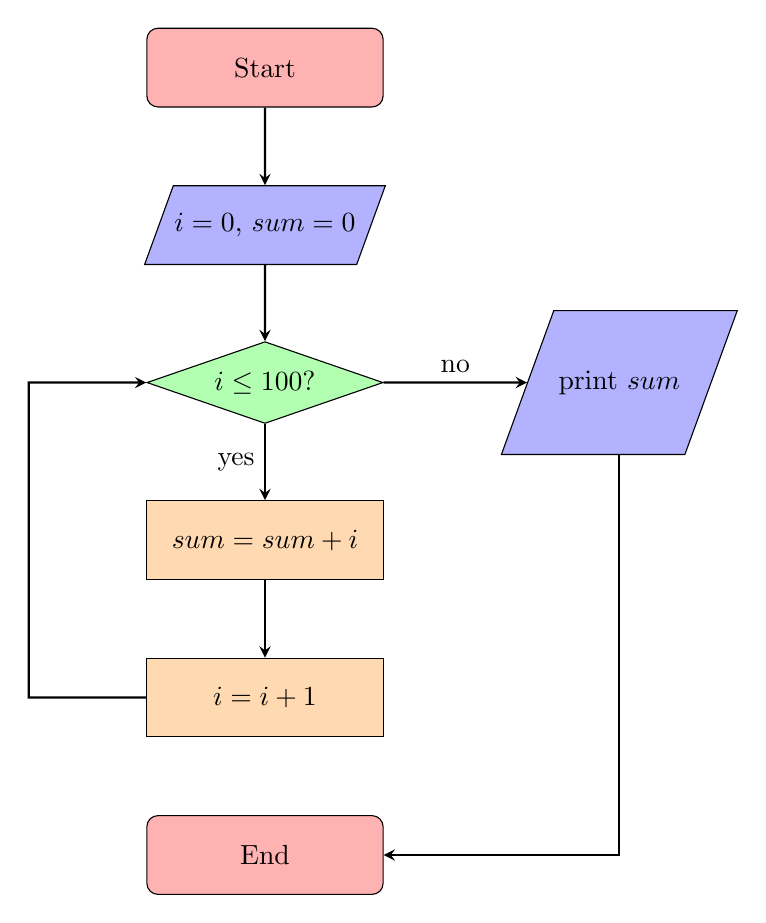
\begin{tikzpicture}[node distance=2cm]
		\node (start) [startend] {Start};
		\node (init) [io, below of=start] {$ i = 0 $, $ sum = 0 $};
		\node (decision)  [decision, below of=init] {$ i \le 100 $?};
		\node (accumulation) [process, below of=decision] {$ sum = sum + i $};
		\node (update) [process, below of=accumulation] {$ i = i + 1 $};
		\node (output) [io, right of=decision, xshift=2.5cm] {print $ sum $};
		\node (end) [startend, below of=update] {End};

		\draw [arrow] (start) -- (init);
		\draw [arrow] (init) -- (decision);
		\draw [arrow] (decision) -- node[anchor=east] {yes } (accumulation);
		\draw [arrow] (accumulation) -- (update);
		\draw [arrow] (update) -- (-3,-8) -- (-3,-4) -- (decision);
		\draw [arrow] (decision) -- node[anchor=south] {no} (output);
		\draw [arrow] (output) |- (end);
	\end{tikzpicture}
	\caption{计算$ \sum_{i=1}^{100} i $的流程图}
\end{figure}

\vspace{0.5cm}

\subsection{Hello World!}

Hello World是学习编程的第一个程序,它的作用是向屏幕输出"Hello World!"。\\

\mybox{Hello World!}

\begin{lstlisting}[language=C++]
#include <iostream>

using namespace std;

int main()
{
	cout << "Hello World!" << endl;
	return 0;
}
\end{lstlisting}

\begin{tcolorbox}
	\mybox{运行结果}
	\begin{verbatim}
Hello World!
	\end{verbatim}
\end{tcolorbox}

\#include <stdio.h>用于包含输入输出库的头文件(header file),这样才能够在程序中进行输入输出相关的操作。\\

using namespace std表示使用std命名空间。\\

main()是程序的入口,程序运行后会首先执行main()中的代码。cout的功能是在屏幕上输出数据,endl表示输出一个换行符。最后的分号用于表示一条语句的结束,注意不要使用中文的分号。\\

return 0表示main()运行结束,返回值为0,一般返回0用于表示程序正常结束。\\

不同编程语言的Hello World写法大同小异,可以看出编程语言的基本结构是相似的。\\

\mybox{C}

\begin{lstlisting}[language=C]
#include <stdio.h>

int main() {
	printf("Hello World!\n");
	return 0;
}
\end{lstlisting}

\vspace{0.5cm}

\mybox{Java}

\begin{lstlisting}[language=Java]
public class HelloWorld {
    public static void main(String[] args) {
        System.out.println("Hello World!");
    }
}
\end{lstlisting}

\vspace{0.5cm}

\mybox{Python}

\begin{lstlisting}[language=Python]
print("Hello World!")
\end{lstlisting}

\vspace{0.5cm}

\subsection{注释(Comment)}

注释就是对代码的解释和说明,它并不会程序所执行。注释能提高程序的可读性,让人更加容易了解代码的功能。\\

注释一般分为单行注释和多行注释:

\begin{enumerate}
	\item 单行注释:以//开头,该行之后的内容视为注释。
	\item 多行注释:以/*开头,*/结束,中间的内容视为注释。
\end{enumerate}

\vspace{0.5cm}

\mybox{注释}

\begin{lstlisting}[language=C++]
/*
* Author: Terry
* Date: 2022/11/16
*/

#include <iostream>      // header file

using namespace std;

int main()
{
	cout << "Hello World!" << endl;
	return 0;
}
\end{lstlisting}

\newpage

\section{数据类型}

\subsection{数据类型(Data Types)}

在计算机中,每个数据一般都有一个对应的类型,基础数据类型包括:

\begin{enumerate}
	\item 整型
	      \begin{itemize}
		      \item 短整型short
		      \item 整型int
		      \item 长整型long
		      \item 长长整型long long
	      \end{itemize}

	\item 浮点型
	      \begin{itemize}
		      \item 单精度浮点数float
		      \item 双精度浮点数double
	      \end{itemize}

	\item 字符型char
\end{enumerate}

\vspace{0.5cm}

不同的数据类型所占的内存空间大小不同,因此所能表示的数值范围也不同。\\

\begin{table}[H]
	\centering
	\setlength{\tabcolsep}{5mm}{
		\begin{tabular}{|c|c|c|}
			\hline
			\textbf{数据类型} & \textbf{大小} & \textbf{取值范围}           \\
			\hline
			short             & 2字节         & $ -2^{15} \sim 2^{15} - 1 $ \\
			\hline
			int               & 4字节         & $ -2^{31} \sim 2^{31} - 1 $ \\
			\hline
			long              & 4字节         & $ -2^{31} \sim 2^{31} - 1 $ \\
			\hline
			long long         & 8字节         & $ -2^{63} \sim 2^{63} - 1 $ \\
			\hline
			float             & 4字节         & 7位有效数字                 \\
			\hline
			double            & 8字节         & 15位有效数字                \\
			\hline
			char              & 1字节         & $ -128 \sim 127 $           \\
			\hline
		\end{tabular}
	}
\end{table}

\vspace{0.5cm}

\subsection{变量(Variable)}

变量是用来存储数据的内存空间,每个变量都有一个类型,变量中只能存储对应类型的数据。

\vspace{-0.5cm}

\begin{lstlisting}[language=C++]
int num = 10;
double salary = 8232.56;
\end{lstlisting}

\vspace{0.5cm}

变量的命名需要符合规范:

\begin{enumerate}
	\item 由字母、数字和下划线组成,不能以数字开头
	\item 不可以使用编程语言中预留的关键字
	\item 使用英语单词,顾名思义
\end{enumerate}

关键字是编程语言内置的一些名称,具有特殊的用处和意义,因此不应该作为变量名,防止产生歧义。\\

\begin{table}[H]
	\centering
	\setlength{\tabcolsep}{5mm}{
		\begin{tabular}{|c|c|c|c|c|}
			\hline
			asm      & auto     & break     & case     & catch    \\
			\hline
			char     & class    & const     & continue & default  \\
			\hline
			delete   & do       & double    & else     & enum     \\
			\hline
			extern   & float    & for       & friend   & goto     \\
			\hline
			if       & inline   & int       & long     & new      \\
			\hline
			operator & private  & protected & public   & register \\
			\hline
			return   & short    & signed    & sizeof   & static   \\
			\hline
			struct   & switch   & template  & this     & throw    \\
			\hline
			try      & typedef  & union     & unsigned & virtual  \\
			\hline
			void     & volatile & while     &          &          \\
			\hline
		\end{tabular}
	}
	\caption{关键字}
\end{table}

\vspace{0.5cm}

\subsection{常量(Constant)}

变量的值在程序运行过程中可以修改,但有一些数据的值是固定的,为了防止这些数据被随意改动,可以将这些数据定义为常量。\\

在数据类型前加上const关键字,即可定义常量,常量一般使用大写表示。如果在程序中尝试修改常量,将会报错。\\

\mybox{常量}

\begin{lstlisting}[language=C++]
#include <iostream>

using namespace std;

int main()
{
	const double PI = 3.1415;
	PI = 4;
	return 0;
}
\end{lstlisting}

\begin{tcolorbox}
	\mybox{运行结果}\\
	\textcolor{red}{error: assignment of read-only variable "PI"}
\end{tcolorbox}

\newpage

\section{输入输出}

\subsection{cout}

cout是输出流对象,用来向屏幕输出数据。但是有些需要输出的字符在编程语言中具有特殊含义,因此这些特殊的字符,需要经过转义后输出。\\

\begin{table}[H]
	\centering
	\setlength{\tabcolsep}{5mm}{
		\begin{tabular}{|c|c|}
			\hline
			\textbf{转义字符}      & \textbf{描述}                \\
			\hline
			\lstinline|\\| & 反斜杠\lstinline|\| \\
			\hline
			\lstinline|\'| & 单引号\lstinline|'| \\
			\hline
			\lstinline|\"| & 双引号\lstinline|"| \\
			\hline
			\lstinline|\n| & 换行                         \\
			\hline
			\lstinline|\t| & 制表符                       \\
			\hline
		\end{tabular}
	}
	\caption{转义字符}
\end{table}

\mybox{转义字符}

\begin{lstlisting}[language=C++]
#include <iostream>

using namespace std;

int main()
{
	cout << "\"Hello\nWorld\"" << endl;
	return 0;
}
\end{lstlisting}

\begin{tcolorbox}
	\mybox{运行结果}
	\begin{verbatim}
"Hello
World"
	\end{verbatim}
\end{tcolorbox}

在对变量的值进行输出时,可以使用格式控制符改变输出的格式。\\

\mybox{长方形面积}

\begin{lstlisting}[language=C++]
#include <iostream>
#include <iomanip>

using namespace std;

int main()
{
	int length = 10;
	int width = 5;
	double area = length * width;

	cout << "Area = " << length << " * " << width << " = "
			<< fixed << setprecision(2) << area << endl;
	return 0;
}
\end{lstlisting}

\begin{tcolorbox}
	\mybox{运行结果}
	\begin{verbatim}
Area = 10 * 5 = 50.00
	\end{verbatim}
\end{tcolorbox}

\vspace{0.5cm}

\subsection{printf()}

printf()是C语言中的输出函数,包含在头文件stdio.h中,用于向屏幕输出指定格式的文本,使用对应类型的占位符可以更加方便地输出变量的值。\\

\begin{table}[H]
	\centering
	\setlength{\tabcolsep}{5mm}{
		\begin{tabular}{|c|c|}
			\hline
			\textbf{数据类型} & \textbf{占位符} \\
			\hline
			int               & \%d             \\
			\hline
			float             & \%f             \\
			\hline
			double            & \%f             \\
			\hline
			char              & \%c             \\
			\hline
		\end{tabular}
	}
	\caption{占位符}
\end{table}

\vspace{-0.5cm}

\begin{lstlisting}[language=C]
printf("Area = %d * %d = %.2f\n", length, width, area);
\end{lstlisting}

\vspace{0.5cm}

\subsection{cin}

有时候一些数据需要从键盘输入,cin可以读取对应类型的数据,并赋值给相应的变量。\\

在使用cin前,通常会使用cout先输出一句提示信息,告诉用户需要输入什么数据。\\

\mybox{圆面积}

\begin{lstlisting}[language=C++]
#include <iostream>
#include <cmath>
#include <iomanip>

using namespace std;

int main()
{
	const double PI = 3.14159;
	double r;
	double area;

	cout << "Radius: ";
	cin >> r;

	area = PI * pow(r, 2);
	cout << "Area = " << fixed << setprecision(2) << area << endl;
	
	return 0;
}
\end{lstlisting}

\begin{tcolorbox}
	\mybox{运行结果}
	\begin{verbatim}
Radius: 5
Area = 78.54
	\end{verbatim}
\end{tcolorbox}

头文件cmath中定义了一些常用的数学函数,例如pow(x, y)可用于计算$ x $的$ y $次方。\\

\newpage

\section{表达式}

\subsection{算术运算符}

大部分编程语言中的除法与数学中的除法意义不同。\\

当相除的两个数都为整数时,那么就会进行整除运算,因此结果仍为整数,例如21 / 4 = 5。\\

如果相除的两个数中至少有一个为浮点数时,那么就会进行普通的除法运算,结果为浮点数,例如21.0 / 4 = 5.25。\\

取模(modulo)运算符\%用于计算两个整数相除之后的余数,例如22 \% 3 = 1、4 \% 7 = 4。\\

\mybox{逆序三位数}

\begin{lstlisting}[language=C++]
#include <iostream>

using namespace std;

int main()
{
	int num;
	int a, b, c;

	cout << "Enter a 3-digit integer: ";
	cin >> num;

	a = num / 100;
	b = num / 10 % 10;
	c = num % 10;

	cout << "Reversed: " << c*100 + b*10 + a << endl;
	return 0;
}
\end{lstlisting}

\begin{tcolorbox}
	\mybox{运行结果}
	\begin{verbatim}
Enter a 3-digit integer: 520
Reversed: 25
	\end{verbatim}
\end{tcolorbox}

\vspace{0.5cm}

\subsection{复合运算符}

使用复合运算符可以使表达式更加简洁。例如\lstinline|a = a + b|可以写成\lstinline|a += b|,-=、*=、/=、\%=等复合运算符的使用方式同理。\\

当需要给一个变量的值加/减1时,除了可以使用\lstinline|a += 1|或\lstinline|a -= 1|之外,还可以使用++或--运算符,但是\lstinline|++|和\lstinline|--|可以出现在变量之前或之后:\\

\begin{table}[H]
	\centering
	\setlength{\tabcolsep}{5mm}{
		\begin{tabular}{|c|l|}
			\hline
			\textbf{表达式}         & \textbf{含义}         \\
			\hline
			\lstinline|a++| & 执行完所在语句后自增1 \\
			\hline
			\lstinline|++a| & 在执行所在语句前自增1 \\
			\hline
			\lstinline|a--| & 执行完所在语句后自减1 \\
			\hline
			\lstinline|--a| & 在执行所在语句前自减1 \\
			\hline
		\end{tabular}
	}
	\caption{自增/自减运算符}
\end{table}

\mybox{自增/自减运算符}

\begin{lstlisting}[language=C++]
#include <iostream>

using namespace std;

int main()
{
	int n = 10;

	cout << n++ << endl;
	cout << ++n << endl;
	cout << n-- << endl;
	cout << --n << endl;

	return 0;
}
\end{lstlisting}

\begin{tcolorbox}
	\mybox{运行结果}
	\begin{verbatim}
10
12
12
10
	\end{verbatim}
\end{tcolorbox}

\vspace{0.5cm}

\subsection{隐式类型转换}

在计算机计算的过程中,只有类型相同的数据才可以进行运算。例如整数+整数、浮点数/浮点数等。\\

但是很多时候,我们仍然可以对不同类型的数据进行运算,而并不会产生错误,例如整数+浮点数。这是由于编译器会自动进行类型转换。在整数+浮点数的例子中,编译器会将整数转换为浮点数,这样就可以进行运算了。\\

编译器选择将整数转换为浮点数,而不是将浮点数转换为整数的原因在于,浮点数相比整数能够表示的范围更大。例如整数8可以使用8.0表示,而浮点数9.28变为整数9后就会丢失精度。\\

隐式类型转换最常见的情形就是除法运算,这也是导致整数/整数=整数、整数/浮点数=浮点数的原因。\\

\subsection{显式类型转换}

有些时候编译器无法自动进行类型转换,这时就需要我们手动地强制类型转换。\\

\mybox{显式类型转换}

\begin{lstlisting}[language=C++]
#include <iostream>
#include <iomanip>

using namespace std;

int main()
{
	int total = 821;
	int num = 10;
	double average = (double)total / num;
	cout << "Average = " << fixed << setprecision(2) << average << endl;
	return 0;
}
\end{lstlisting}

\begin{tcolorbox}
	\mybox{运行结果}
	\begin{verbatim}
Average = 82.10
	\end{verbatim}
\end{tcolorbox}

\newpage
\chapter{分支}

\section{逻辑运算符}

\subsection{关系运算符}

编程中经常需要使用关系运算符来比较两个数据的大小,比较的结果是一个布尔值(boolean),即True(非0)或False(0)。\\

在编程中需要注意,一个等号=表示赋值运算,而两个等号==表示比较运算。\\

\begin{table}[H]
	\centering
	\setlength{\tabcolsep}{5mm}{
		\begin{tabular}{|c|c|}
			\hline
			\textbf{数学符号} & \textbf{关系运算符} \\
			\hline
			$ < $             & <                   \\
			\hline
			$ > $             & >                   \\
			\hline
			$ \le $           & <=                  \\
			\hline
			$ \ge $           & >=                  \\
			\hline
			$ = $             & ==                  \\
			\hline
			$ \ne $           & !=                  \\
			\hline
		\end{tabular}
	}
\end{table}

\vspace{0.5cm}

\subsection{逻辑运算符}

逻辑运算符用于连接多个关系表达式,其结果也是一个布尔值。\\

\begin{enumerate}
	\item 逻辑与\&\&:当多个条件全部为True,结果为True。\\
	      \begin{table}[H]
		      \centering
		      \setlength{\tabcolsep}{5mm}{
			      \begin{tabular}{|c|c|c|}
				      \hline
				      \textbf{条件1} & \textbf{条件2} & \textbf{条件1 \&\& 条件2} \\
				      \hline
				      T              & T              & T                         \\
				      \hline
				      T              & F              & F                         \\
				      \hline
				      F              & T              & F                         \\
				      \hline
				      F              & F              & F                         \\
				      \hline
			      \end{tabular}
		      }
	      \end{table}

	\item 逻辑或||:多个条件至少有一个为True时,结果为True。\\
	      \begin{table}[H]
		      \centering
		      \setlength{\tabcolsep}{5mm}{
			      \begin{tabular}{|c|c|c|}
				      \hline
				      \textbf{条件1} & \textbf{条件2} & \textbf{条件1 || 条件2} \\
				      \hline
				      T              & T              & T                       \\
				      \hline
				      T              & F              & T                       \\
				      \hline
				      F              & T              & T                       \\
				      \hline
				      F              & F              & F                       \\
				      \hline
			      \end{tabular}
		      }
	      \end{table}

	\item 逻辑非!:条件为True时,结果为False;条件为False时,结果为True。\\
	      \begin{table}[H]
		      \centering
		      \setlength{\tabcolsep}{5mm}{
			      \begin{tabular}{|c|c|}
				      \hline
				      \textbf{条件} & \textbf{!条件} \\
				      \hline
				      T             & F              \\
				      \hline
				      F             & T              \\
				      \hline
			      \end{tabular}
		      }
	      \end{table}
\end{enumerate}

\newpage

\section{if}

\subsection{if}

if语句用于判断一个条件是否成立,如果成立则进入语句块,否则不执行。\\

\mybox{年龄}

\begin{lstlisting}[language=C++]
#include <iostream>

using namespace std;

int main()
{
	int age;
	cout << "Enter your age: ";
	cin >> age;
	if(age > 0 && age < 18)
	{
		cout << "Minor" << endl;
	}
	return 0;
}
\end{lstlisting}

\begin{tcolorbox}
	\mybox{运行结果}
	\begin{verbatim}
Enter your age: 17
Minor
\end{verbatim}
\end{tcolorbox}

\vspace{0.5cm}

\subsection{if-else}

if-else的结构与if类似,只是在if语句块中的条件不成立时,执行else语句块中的语句。\\

\mybox{闰年}

\begin{lstlisting}[language=C++]
#include <iostream>

using namespace std;

int main()
{
	int year;
	cout << "Enter a year: ";
	cin >> year;

	/*
		* A year is a leap year if it is
		* 1. exactly divisible by 4, and not divisible by 100;
		* 2. or is exactly divisible by 400
		*/
	if((year % 4 == 0 && year % 100 != 0) || year % 400 == 0)
	{
		cout << "Leap year" << endl;
	}
	else
	{
		cout << "Common year" << endl;
	}

	return 0;
}
\end{lstlisting}

\begin{tcolorbox}
	\mybox{运行结果}
	\begin{verbatim}
Enter a year: 2020
Leap year
\end{verbatim}
\end{tcolorbox}

\vspace{0.5cm}

\subsection{if-else if-else}

当需要对更多的条件进行判断时,可以使用if-else if-else语句。\\

\mybox{字符}

\begin{lstlisting}[language=C++]
#include <iostream>

using namespace std;

int main()
{
	char c;
	cout << "Enter a character: ";
	cin >> c;

	if(c >= 'a' && c <= 'z')
	{
		cout << "Lowercase" << endl;
	}
	else if(c >= 'A' && c <= 'Z')
	{
		cout << "Uppercase" << endl;
	}
	else if(c >= '0' && c <= '9')
	{
		cout << "Digit" << endl;
	}
	else
	{
		cout << "Special character" << endl;
	}
	
	return 0;
}
\end{lstlisting}

\begin{tcolorbox}
	\mybox{运行结果}
	\begin{verbatim}
Enter a character: T
Uppercase
\end{verbatim}
\end{tcolorbox}

\newpage

\section{switch}

\subsection{switch}

switch结构用于根据一个整数值,选择对应的case执行。需要注意的是,当对应的case中的代码被执行完后,并不会像if语句一样跳出switch结构,而是会继续向后执行,直到遇到break。\\

\mybox{计算器}

\begin{lstlisting}[language=C++]
#include <iostream>

using namespace std;

int main() {
	int num1, num2;
	char op;

	cout << "Enter an expression: ";
	cin >> num1 >> op >> num2;

	switch (op)
	{
	case '+':
		cout << num1 << " + " << num2 << " = " << num1 + num2 << endl;
		break;
	case '-':
		cout << num1 << " - " << num2 << " = " << num1 - num2 << endl;
		break;
	case '*':
		cout << num1 << " * " << num2 << " = " << num1 * num2 << endl;
		break;
	case '/':
		cout << num1 << " / " << num2 << " = " << num1 / num2 << endl;
		break;
	default:
		cout << "Error! Operator is not supported" << endl;
		break;
	}

	return 0;
}
\end{lstlisting}

\begin{tcolorbox}
	\mybox{运行结果}
	\begin{verbatim}
Enter an expression: 5 * 8
5 * 8 = 40
\end{verbatim}
\end{tcolorbox}

\newpage
\chapter{循环}

\section{while}

\subsection{while}

while循环会对条件进行判断,如果条件成立,就会执行循环体,然后再次判断条件,直到条件不成立。\\

while循环的次数由循环变量的变化决定,因此while循环一般都包括对循环变量的初值、判断和更新。

\vspace{-0.5cm}

\begin{lstlisting}[language=C++]
int i = 1;          // initial value
while(i <= 5)       // condition
{
    cout << "In loop: i = " << i << endl;
    i++;            // update
}
cout << "After loop: i = " << i << endl;
\end{lstlisting}

while循环的特点是先判断、再执行,因此循环体有可能会执行一次或多次,也有可能一次也不会执行。\\

\mybox{平均身高}

\begin{lstlisting}[language=C++]
#include <iostream>
#include <iomanip>

#define NUM_PEOPLE 5

using namespace std;

int main()
{
    double height;
    double total = 0;

    int i = 1;
    while (i <= NUM_PEOPLE)
    {
        cout << "Enter person " << i << "'s height: ";
        cin >> height;
        total += height;
        i++;
    }

    double average = total / NUM_PEOPLE;
    cout << "Average height: "
         << fixed << setprecision(2) << average << endl;
    
    return 0;
}
\end{lstlisting}

\begin{tcolorbox}
    \mybox{运行结果}
    \begin{verbatim}
Enter person 1's height: 160.8
Enter person 2's height: 175.2
Enter person 3's height: 171.2
Enter person 4's height: 181.3
Enter person 5's height: 164
Average height: 170.50
\end{verbatim}
\end{tcolorbox}

\vspace{0.5cm}

\mybox{统计元音、辅音数量}

\begin{lstlisting}[language=C++]
#include <iostream>

using namespace std;

int main()
{
    char c;
    int vowel = 0;
    int consonant = 0;

    cout << "Enter an English sentence: ";

    while((c = cin.get()) != '\n')
    {
        if (c == 'a' || c == 'A' ||
            c == 'e' || c == 'E' || 
            c == 'i' || c == 'I' || 
            c == 'o' || c == 'O' || 
            c == 'u' || c == 'U')
        {
            vowel++;
        }
        else if ((c >= 'a' && c <= 'z') || (c >= 'A' && c <= 'Z'))
        {
            consonant++;
        }
    }

    cout << "Vowel = " << vowel << endl;
    cout << "Consonant = " << consonant << endl;
    return 0;
}
\end{lstlisting}

\begin{tcolorbox}
    \mybox{运行结果}
    \begin{verbatim}
Enter an English sentence: Hello World!
Vowel = 3
Consonant = 7
\end{verbatim}
\end{tcolorbox}

\vspace{0.5cm}

\subsection{do-while}

do-while循环是先执行一轮循环体内的代码后,再检查循环的条件是否成立。如果成立,则继续下一轮循环;否则循环结束。\\

do-while循环是先执行、再判断,因此它至少会执行一轮循环。do-while一般应用在一些可能会需要重复,但必定会发生一次的情景下。例如登录账户,用户输入账户和密码后,检查是否正确,如果正确,那么就成功登录;否则继续循环让用户重新输入。\\

需要注意,do-while循环的最后有一个分号。

\vspace{-0.5cm}

\begin{lstlisting}[language=C++]
do {
    // code
} while(condition);
\end{lstlisting}

\vspace{0.5cm}

\mybox{整数位数}

\begin{lstlisting}[language=C++]
#include <iostream>

using namespace std;

int main()
{
    int num;
    int n = 0;

    cout << "Enter an integer: ";
    cin >> num;

    do
    {
        num /= 10;
        n++;
    } while(num != 0);

    cout << "Digits: " << n << endl;
    return 0;
}
\end{lstlisting}

\begin{tcolorbox}
    \mybox{运行结果}
    \begin{verbatim}
Enter an integer: 123
Digits: 3
\end{verbatim}
\end{tcolorbox}

\vspace{0.5cm}

\mybox{猜数字}

\begin{lstlisting}[language=C++]
#include <iostream>
#include <cstdlib>
#include <ctime>

using namespace std;

int main()
{
    srand(time(NULL));          // set random seed

    // generate random number between 1 and 100
    int answer = rand() % 100 + 1;
    int num = 0;
    int cnt = 0;

    do
    {
        cout << "Guess a number: ";
        cin >> num;
        cnt++;
        
        if(num > answer)
        {
            cout << "Too high" << endl;
        }
        else if(num < answer)
        {
            cout << "Too low" << endl;
        }
    } while(num != answer);

    cout << "Correct! You guessed " << cnt << " times." << endl;
    return 0;
}
\end{lstlisting}

\begin{tcolorbox}
    \mybox{运行结果}
    \begin{verbatim}
Guess a number: 50
Too high
Guess a number: 25
Too low
Guess a number: 37
Too low
Guess a number: 43
Too high
Guess a number: 40
Too high
Guess a number: 38
Too low
Guess a number: 39
Correct! You guessed 7 times.
\end{verbatim}
\end{tcolorbox}

\newpage

\section{for}

\subsection{for}

while循环将循环变量的初值、条件和更新写在了三个地方,但是这样不容易明显地看出循环变量的变化。\\

for循环将循环变量的初值、条件和更新写在了一行内,中间用分号隔开。对于指定次数的循环一般更多地会采用for循环,而对于不确定次数的一般会采用while循环。

\vspace{-0.5cm}

\begin{lstlisting}[language=C++]
for(int i = 0; i < 5; i++)
{
    cout << "i = " << i << endl;
}
\end{lstlisting}

\vspace{0.5cm}

\mybox{累加}

\begin{lstlisting}[language=C++]
#include <iostream>

using namespace std;

int main()
{
    int sum = 0;
    for(int i = 1; i <= 100; i++)
    {
        sum += i;
    }
    cout << "Sum = " << sum << endl;
    return 0;
}
\end{lstlisting}

\begin{tcolorbox}
    \mybox{运行结果}
    \begin{verbatim}
Sum = 5050
\end{verbatim}
\end{tcolorbox}

\vspace{0.5cm}

\mybox{斐波那契数列}

\begin{figure}[H]
    \centering
    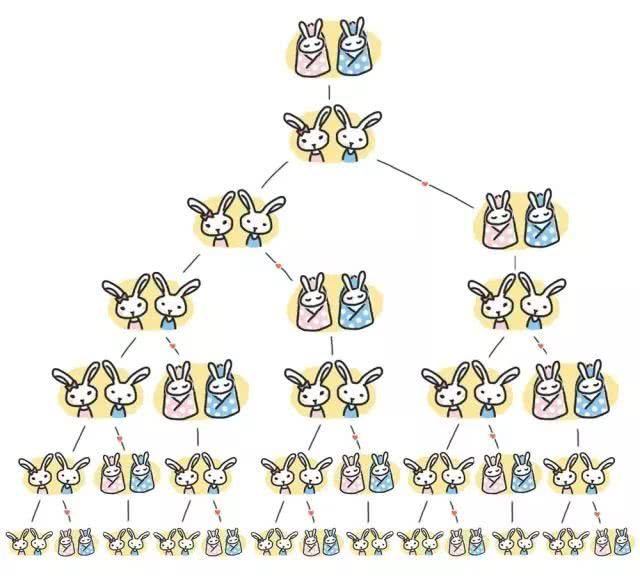
\includegraphics[scale=0.5]{img/Chapter3/3-2/1.png}
\end{figure}

\begin{lstlisting}[language=C++]
#include <iostream>

using namespace std;

int main()
{
    int n;
    cout << "Enter the number of terms: ";
    cin >> n;

    if(n == 1)
    {
        cout << "1" << endl;
    }
    else if(n == 2)
    {
        cout << "1, 1" << endl;
    }
    else
    {
        int num1, num2, val;
        num1 = 1;
        num2 = 1;
        cout << "1, 1";

        for(int i = 3; i <= n; i++)
        {
            val = num1 + num2;
            cout << ", " << val;
            num1 = num2;
            num2 = val;
        }
        cout << endl;
    }
    
    return 0;
}
\end{lstlisting}

\begin{tcolorbox}
    \mybox{运行结果}
    \begin{verbatim}
Enter the number of terms: 10
1, 1, 2, 3, 5, 8, 13, 21, 34, 55
\end{verbatim}
\end{tcolorbox}

\vspace{0.5cm}

\subsection{嵌套循环}

循环也可以嵌套使用,外层循环每执行一次,内层循环就会执行多次。

\vspace{-0.5cm}

\begin{lstlisting}[language=C++]
for(int i = 0; i < 2; i++)
{
    for(int j = 0; j < 3; j++)
    {
        cout << "i = " << i << ", j = " << j << endl;
    }
}
\end{lstlisting}

\begin{tcolorbox}
    \mybox{运行结果}
    \begin{verbatim}
i = 0, j = 0
i = 0, j = 1
i = 0, j = 2
i = 1, j = 0
i = 1, j = 1
i = 1, j = 2
\end{verbatim}
\end{tcolorbox}

\vspace{0.5cm}

\mybox{九九乘法表}\\

\begin{table}[H]
    \centering
    \setlength{\tabcolsep}{1.5mm}{
        \begin{tabular}{|c|c|c|c|c|c|c|c|c|}
            \hline
            1*1=1 & 1*2=2  & 1*3=3  & 1*4=4  & 1*5=5  & 1*6=6  & 1*7=7  & 1*8=8  & 1*9=9  \\
            \hline
            2*1=2 & 2*2=4  & 2*3=6  & 2*4=8  & 2*5=10 & 2*6=12 & 2*7=14 & 2*8=16 & 2*9=18 \\
            \hline
            3*1=3 & 3*2=6  & 3*3=9  & 3*4=12 & 3*5=15 & 3*6=18 & 3*7=21 & 3*8=24 & 3*9=27 \\
            \hline
            4*1=4 & 4*2=8  & 4*3=12 & 4*4=16 & 4*5=20 & 4*6=24 & 4*7=28 & 4*8=32 & 4*9=36 \\
            \hline
            5*1=5 & 5*2=10 & 5*3=15 & 5*4=20 & 5*5=25 & 5*6=30 & 5*7=35 & 5*8=40 & 5*9=45 \\
            \hline
            6*1=6 & 6*2=12 & 6*3=18 & 6*4=24 & 6*5=30 & 6*6=36 & 6*7=42 & 6*8=48 & 6*9=54 \\
            \hline
            7*1=7 & 7*2=14 & 7*3=21 & 7*4=28 & 7*5=35 & 7*6=42 & 7*7=49 & 7*8=56 & 7*9=63 \\
            \hline
            8*1=8 & 8*2=16 & 8*3=24 & 8*4=32 & 8*5=40 & 8*6=48 & 8*7=56 & 8*8=64 & 8*9=72 \\
            \hline
            9*1=9 & 9*2=18 & 9*3=27 & 9*4=36 & 9*5=45 & 9*6=54 & 9*7=63 & 9*8=72 & 9*9=81 \\
            \hline
        \end{tabular}
    }
\end{table}

\begin{lstlisting}[language=C++]
#include <iostream>

using namespace std;

int main()
{
    for(int i = 1; i <= 9; i++)
    {
        for(int j = 1; j <= 9; j++)
        {
            cout << i << "*" << j << "=" << i*j << "\t";
        }
        cout << endl;
    }
    return 0;
}
\end{lstlisting}

\vspace{0.5cm}

\mybox{打印图案}

\begin{lstlisting}
*
**
***
****
*****
\end{lstlisting}

\begin{lstlisting}[language=C++]
#include <iostream>

using namespace std;

int main()
{
    for(int i = 1; i <= 5; i++)
    {
        for(int j = 1; j <= i; j++)
        {
            cout << "*";
        }
        cout << endl;
    }
    return 0;
}
\end{lstlisting}

\newpage

\section{break or continue?}

\subsection{break}

break可用于跳出当前的switch或循环结构。在一些情况下,在循环的中途已经完成了某个目标,没有必要再进行剩余的循环,这时就可以使用break跳出循环。\\

例如在判断一个数$ n $是否为素数时,利用循环逐个判断$ 2 \sim n - 1 $之间的数是否能整除$ n $。只要发现其中有一个数能整除$ n $,就证明$ n $不是素数,可以跳出循环,不必再进行剩余的检查。\\

\mybox{素数}

\begin{lstlisting}[language=C++]
#include <iostream>
#include <cmath>

using namespace std;

int main()
{
    int n;
    cout << "Enter an integer: ";
    cin >> n;

    bool is_prime = true;
    for(int i = 2; i <= sqrt(n); i++)
    {
        if(n % i == 0)
        {
            is_prime = false;
            break;
        }
    }

    if(is_prime)
    {
        cout << n << " is a prime number" << endl;
    }
    else
    {
        cout << n << " is not a prime number" << endl;
    }

    return 0;
}
\end{lstlisting}

\begin{tcolorbox}
    \mybox{运行结果}
    \begin{verbatim}
Enter an integer: 17
17 is a prime number
\end{verbatim}
\end{tcolorbox}

\vspace{0.5cm}

\subsection{continue}

continue与break使用方法类似,但是它并不是跳出循环,而是跳过本轮循环,直接开始下一轮循环。\\

\mybox{正数平方和}

\begin{lstlisting}[language=C]
#include <iostream>

using namespace std;

int main()
{
    int n = 10;
    cout << "Enter " << n << " integers: ";

    int sum_square = 0;
    for(int i = 0; i < n; i++)
    {
        int num;
        cin >> num;
        if(num < 0)
        {
            continue;
        }

        sum_square += num * num;
    }

    cout << "Sum of squares of positive integers: "
            << sum_square << endl;
            
    return 0;
}
\end{lstlisting}

\begin{tcolorbox}
    \mybox{运行结果}
    \begin{verbatim}
Enter 10 integers: 5 7 -2 0 4 -4 -9 3 9 5
Sum of squares of positive integers: 205
\end{verbatim}
\end{tcolorbox}

\newpage
\chapter{数组}

\section{数组}

\subsection{数组(Array)}

数组能够存储一组类型相同的元素,数组在声明时必须指定它的大小(容量),数组的大小是固定的,无法在运行时动态改变。数组通过下标(index)来访问某一位置上的元素,下标从0开始。

\vspace{-0.5cm}

\begin{lstlisting}[language=C]
int arr[5] = {3, 6, 8, 2, 4};
\end{lstlisting}

\begin{figure}[H]
	\centering
	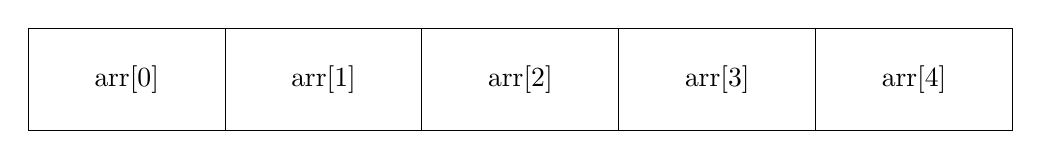
\begin{tikzpicture}[scale=0.5]
		\draw[-] (0,0) -- (5,0) -- (10,0) -- (15,0) -- (20,0) -- (25,0) -- (25,2.6) -- (20,2.6) -- (15,2.6) -- (10,2.6) -- (5,2.6) -- (0,2.6) -- (0,0);
		\draw[-] (5,0) -- (5,2.6);
		\draw[-] (10,0) -- (10,2.6);
		\draw[-] (15,0) -- (15,2.6);
		\draw[-] (20,0) -- (20,2.6);

		\draw (2.5,1.3) node {arr[0]};
		\draw (7.5,1.3) node {arr[1]};
		\draw (12.5,1.3) node {arr[2]};
		\draw (17.5,1.3) node {arr[3]};
		\draw (22.5,1.3) node {arr[4]};
	\end{tikzpicture}
\end{figure}

如果在声明数组时没有指定数组的大小,那么将根据初始化的元素个数来确定。

\vspace{-0.5cm}

\begin{lstlisting}[language=C]
int arr[] = {3, 6, 8, 2, 4, 0, 1, 7};
\end{lstlisting}

通过下标可以访问数组中的元素,下标的有效范围是0 $ \sim $ 数组的长度 - 1,如果使用不合法的下标就会导致数组越界。

\vspace{-0.5cm}

\begin{lstlisting}[language=C]
printf("%d\n", arr[0]);		// 3
printf("%d\n", arr[3]);		// 2
printf("%d\n", arr[7]);		// 7
\end{lstlisting}

当数组的容量比较大时,可以使用循环来初始化数组。

\vspace{-0.5cm}

\begin{lstlisting}[language=C]
int arr[10];

for(int i = 0; i < 10; i++) {
	arr[i] = i + 1;
}
\end{lstlisting}

\vspace{0.5cm}

\mybox{查找数据}

\begin{lstlisting}[language=C]
#include <stdio.h>
#include <stdbool.h>

int main() {
	int n;
	printf("Enter the number of elements: ");
	scanf("%d", &n);

	int arr[n];
	printf("Enter the elements: ");
	for (int i = 0; i < n; i++) {
		scanf("%d", &arr[i]);
	}

	int key;
	printf("Enter the key: ");
	scanf("%d", &key);

	bool found = false;
	for (int i = 0; i < n; i++) {
		if (arr[i] == key) {
			found = true;
			break;
		}
	}

	if (found) {
		printf("%d exists.\n", key);
	} else {
		printf("%d not found!\n", key);
	}

	return 0;
}
\end{lstlisting}

\begin{tcolorbox}
	\mybox{运行结果}
	\begin{verbatim}
Enter the number of elements: 5
Enter the elements: 4 8 9 2 3
Enter the key: 2
2 exists.
	\end{verbatim}
\end{tcolorbox}

\vspace{0.5cm}

\mybox{最大值/最小值}

\begin{lstlisting}[language=C]
#include <stdio.h>

int main() {
	int num[] = {7, 6, 2, 9, 3, 1, 4, 0, 5, 8};
	int n = sizeof(num) / sizeof(num[0]);
	int max = num[0];
	int min = num[0];

	for(int i = 1; i < n; i++) {
		if(num[i] > max) {
			max = num[i];
		}
		if(num[i] < min) {
			min = num[i];
		}
	}

	printf("Max = %d\n", max);
	printf("Min = %d\n", min);
	return 0;
}
\end{lstlisting}

\begin{tcolorbox}
	\mybox{运行结果}
	\begin{verbatim}
Max = 9
Min = 0
	\end{verbatim}
\end{tcolorbox}

\vspace{0.5cm}

\subsection{二维数组(2-Dimensional Array)}

二维数组由行和列两个维度组成,行和列的下标同样也都是从0开始。在声明二维数组时,需要指定行和列的大小。二维数组可以看成是由多个一维数组组成的,因此二维数组中的每个元素都是一个一维数组。

\vspace{-0.5cm}

\begin{lstlisting}[language=C]
int arr[3][4] = {{1, 2, 3, 4}, {5, 6, 7, 8}, {9, 10, 11, 12}};
\end{lstlisting}

\begin{table}[H]
	\centering
	\setlength{\tabcolsep}{5mm}{
		\begin{tabular}{|c|c|c|c|}
			\hline
			arr[0][0] & arr[0][1] & arr[0][2] & arr[0][3] \\
			\hline
			arr[1][0] & arr[1][1] & arr[1][2] & arr[1][3] \\
			\hline
			arr[2][0] & arr[2][1] & arr[2][2] & arr[2][3] \\
			\hline
		\end{tabular}
	}
\end{table}

在初始化二维数组时,为了能够更直观地看出二维数组的结构,可以将每一行单独写在一行中。

\vspace{-0.5cm}

\begin{lstlisting}[language=C]
int arr[3][4] = {
	{1, 2, 3, 4},
	{5, 6, 7, 8},
	{9, 10, 11, 12},
};
\end{lstlisting}

对于容量较大的二维数组,可以通过两层循环进行初始化。

\vspace{-0.5cm}

\begin{lstlisting}[language=C]
int arr[3][4];

for(int i = 0; i < 3; i++) {
	for(int j = 0; j < 4; j++) {
		arr[i][j] = 0;
	}
}
\end{lstlisting}

\vspace{0.5cm}

\mybox{矩阵运算}

\begin{align}\nonumber
	\left[\begin{matrix}
			1 & 3 \\
			1 & 0 \\
			1 & 2 \\
		\end{matrix} \right]
	+
	\left[\begin{matrix}
			0 & 0 \\
			7 & 5 \\
			2 & 1 \\
		\end{matrix} \right]
	=
	\left[\begin{matrix}
			1+0 & 3+0 \\
			1+7 & 0+5 \\
			1+2 & 2+1 \\
		\end{matrix} \right]
	=
	\left[\begin{matrix}
			1 & 3 \\
			8 & 5 \\
			3 & 3 \\
		\end{matrix} \right]
\end{align}

\begin{align}\nonumber
	\left[\begin{matrix}
			1 & 3 \\
			1 & 0 \\
			1 & 2 \\
		\end{matrix} \right]
	-
	\left[\begin{matrix}
			0 & 0 \\
			7 & 5 \\
			2 & 1 \\
		\end{matrix} \right]
	=
	\left[\begin{matrix}
			1-0 & 3-0 \\
			1-7 & 0-5 \\
			1-2 & 2-1 \\
		\end{matrix} \right]
	=
	\left[\begin{matrix}
			1  & 3  \\
			-6 & -5 \\
			-1 & 1  \\
		\end{matrix} \right]
\end{align}

\begin{lstlisting}[language=C]
#include <stdio.h>

int main() {
	int A[3][2] = {
		{1, 3},
		{1, 0},
		{1, 2}
	};
	int B[3][2] = {
		{0, 0},
		{7, 5},
		{2, 1}
	};
	int C[3][2];

	printf("Matrix Addition\n");
	for(int i = 0; i < 3; i++) {
		for(int j = 0; j < 2; j++) {
			C[i][j] = A[i][j] + B[i][j];
			printf("%3d", C[i][j]);
		}
		printf("\n");
	}
	
	printf("Matrix Subtraction\n");
	for(int i = 0; i < 3; i++) {
		for(int j = 0; j < 2; j++) {
			C[i][j] = A[i][j] - B[i][j];
			printf("%3d", C[i][j]);
		}
		printf("\n");
	}
	
	return 0;
}
\end{lstlisting}

\begin{tcolorbox}
	\mybox{运行结果}
	\begin{verbatim}
Matrix Addition
  1  3
  8  5
  3  3
Matrix Subtraction
  1  3
  -6 -5
  -1  1
	\end{verbatim}
\end{tcolorbox}

\newpage

\section{字符串}

\subsection{ASCII}

美国信息交换标准代码ASCII(American Standard Code for Information Interchange)一共定义了128个字符。\\

\begin{longtable}{|c|c|c|c|c|c|c|c|}
	\hline
	\textbf{ASCII} & \textbf{字符} & \textbf{ASCII} & \textbf{字符} & \textbf{ASCII} & \textbf{字符}          & \textbf{ASCII} & \textbf{字符}          \\
	\hline
	0              & NUT           & 32             & (space)       & 64             & @                      & 96             & \lstinline|`| \\
	\hline
	1              & SOH           & 33             & !             & 65             & A                      & 97             & a                      \\
	\hline
	2              & STX           & 34             & \text{"}      & 66             & B                      & 98             & b                      \\
	\hline
	3              & ETX           & 35             & \#            & 67             & C                      & 99             & c                      \\
	\hline
	4              & EOT           & 36             & \$            & 68             & D                      & 100            & d                      \\
	\hline
	5              & ENQ           & 37             & \%            & 69             & E                      & 101            & e                      \\
	\hline
	6              & ACK           & 38             & \&            & 70             & F                      & 102            & f                      \\
	\hline
	7              & BEL           & 39             & \text{'}      & 71             & G                      & 103            & g                      \\
	\hline
	8              & BS            & 40             & (             & 72             & H                      & 104            & h                      \\
	\hline
	9              & HT            & 41             & )             & 73             & I                      & 105            & i                      \\
	\hline
	10             & LF            & 42             & *             & 74             & J                      & 106            & j                      \\
	\hline
	11             & VT            & 43             & +             & 75             & K                      & 107            & k                      \\
	\hline
	12             & FF            & 44             & ,             & 76             & L                      & 108            & l                      \\
	\hline
	13             & CR            & 45             & -             & 77             & M                      & 109            & m                      \\
	\hline
	14             & SO            & 46             & .             & 78             & N                      & 110            & n                      \\
	\hline
	15             & SI            & 47             & /             & 79             & O                      & 111            & o                      \\
	\hline
	16             & DLE           & 48             & 0             & 80             & P                      & 112            & p                      \\
	\hline
	17             & DC1           & 49             & 1             & 81             & Q                      & 113            & q                      \\
	\hline
	18             & DC2           & 50             & 2             & 82             & R                      & 114            & r                      \\
	\hline
	19             & DC3           & 51             & 3             & 83             & S                      & 115            & s                      \\
	\hline
	20             & DC4           & 52             & 4             & 84             & T                      & 116            & t                      \\
	\hline
	21             & NAK           & 53             & 5             & 85             & U                      & 117            & u                      \\
	\hline
	22             & SYN           & 54             & 6             & 86             & V                      & 118            & v                      \\
	\hline
	23             & TB            & 55             & 7             & 87             & W                      & 119            & w                      \\
	\hline
	24             & CAN           & 56             & 8             & 88             & X                      & 120            & x                      \\
	\hline
	25             & EM            & 57             & 9             & 89             & Y                      & 121            & y                      \\
	\hline
	26             & SUB           & 58             & :             & 90             & Z                      & 122            & z                      \\
	\hline
	27             & ESC           & 59             & ;             & 91             & [                      & 123            & \{                     \\
			\hline
	28             & FS            & 60             & <             & 92             & $ \backslash $         & 124            & |                      \\
			\hline
	29             & GS            & 61             & =             & 93             & ]                      & 125            & \}                     \\
	\hline
	30             & RS            & 62             & >             & 94             & \lstinline|^| & 126            & \lstinline|~| \\
	\hline
	31             & US            & 63             & ?             & 95             & \_                     & 127            & DEL                    \\
	\hline
\end{longtable}

\vspace{0.5cm}

\mybox{ASCII}

\begin{lstlisting}[language=C]
#include <stdio.h>

int main() {
	for(int i = 0; i < 128; i++) {
		printf("%d - %c\n", i, i);
	}
	return 0;
}
\end{lstlisting}

\vspace{0.5cm}

\subsection{字符串(String)}

字符数组通常被称为字符串,字符串有两种初始化的方式。一种与普通数组的初始化类似,逐个写出每一个字符,最后需要手动添加$ \backslash $0字符,表示字符串的结束符;另一种是直接使用双引号,这种写法无需手动添加$ \backslash $0。

\vspace{-0.5cm}

\begin{lstlisting}[language=C]
char str[8] = {'p', 'r', 'o', 'g', 'r', 'a', 'm', '\0'};
char str[8] = "program";
\end{lstlisting}

$ \backslash $0占一个字符的大小,因此在设置字符串的大小时需要考虑$ \backslash $0。\\

占位符\%s可以对字符串进行输入输出操作,使用scanf()和gets()都可以用于读取字符串,但是scanf()只会读取到空格为止,而gets()会读取到回车为止。\\

\mybox{字符串输入输出}

\begin{lstlisting}[language=C]
#include <stdio.h>

int main() {
	char str1[32];
	printf("Enter string 1: ");
	gets(str1);
	puts(str1);

	char str2[32];
	printf("Enter string 2: ");
	scanf("%s", str2);
	printf("%s\n", str2);

	return 0;
}
\end{lstlisting}

\begin{tcolorbox}
	\mybox{运行结果}
	\begin{verbatim}
Enter string 1: hello world
hello world
Enter string 2: hello world
hello
	\end{verbatim}
\end{tcolorbox}

\vspace{0.5cm}

\mybox{字符统计}

\begin{lstlisting}[language=C]
#include <stdio.h>

int main() {
	char str[32];
	printf("Enter a string: ");
	gets(str);
	printf("Character to search: ");
	char c = getchar();

	int cnt = 0;
	int i = 0;
	while (str[i] != '\0') {
		if (str[i] == c) {
			cnt++;
		}
		i++;
	}

	printf("\'%c\' appears %d times in \"%s\".\n", c, cnt, str);
	return 0;
}
\end{lstlisting}

\begin{tcolorbox}
	\mybox{运行结果}
	\begin{verbatim}
Enter a string: this is a test
Character to search: t
't' appears 3 times in "this is a test".
	\end{verbatim}
\end{tcolorbox}

\vspace{0.5cm}

\subsection{字符串函数}

头文件<string.h>中定义了一些常用的字符串处理函数。

\subsubsection{strlen()}

计算字符串的长度。\\

\mybox{strlen()}

\begin{lstlisting}[language=C]
#include <stdio.h>
#include <string.h>

int main() {
	char s[] = "hello world";
	printf("Length: %d\n", strlen(s));
	return 0;
}
\end{lstlisting}

\begin{tcolorbox}
	\mybox{运行结果}
	\begin{verbatim}
Length: 11
	\end{verbatim}
\end{tcolorbox}

\vspace{0.5cm}

\subsubsection{strcpy()}

字符串复制,调用者需要确保字符串的大小足够。\\

\mybox{strcpy()}

\begin{lstlisting}[language=C]
#include <stdio.h>
#include <string.h>

int main() {
	char s1[32] = "hello world";
	char s2[32] = "program";

	strcpy(s1, s2);
	printf("s1 = %s\n", s1);
	printf("s2 = %s\n", s2);
	return 0;
}
\end{lstlisting}

\begin{tcolorbox}
	\mybox{运行结果}
	\begin{verbatim}
s1 = program
s2 = program
	\end{verbatim}
\end{tcolorbox}

\vspace{0.5cm}

\subsubsection{strcat()}

字符串拼接,调用者需要确保字符串的大小足够。\\

\mybox{strcat()}

\begin{lstlisting}[language=C]
#include <stdio.h>
#include <string.h>

int main() {
	char s1[32] = "hello";
	char s2[32] = "world";

	strcat(s1, s2);
	printf("s1 = %s\n", s1);
	printf("s2 = %s\n", s2);
	return 0;
}
\end{lstlisting}

\begin{tcolorbox}
	\mybox{运行结果}
	\begin{verbatim}
s1 = helloworld
s2 = world
	\end{verbatim}
\end{tcolorbox}

\vspace{0.5cm}

\subsubsection{strcmp()}

字符串比较,依次比较字符串中每个字符的ASCII码值。通过判断strcmp()的返回值,可以得知两个字符串比较后的结果。

\begin{itemize}
	\item 负数:字符串1 < 字符串2
	\item 正数:字符串1 > 字符串2
	\item 0:字符串1 == 字符串2
\end{itemize}

\vspace{0.5cm}

\mybox{strcmp()}

\begin{lstlisting}[language=C]
#include <stdio.h>
#include <string.h>

int main() {
	char s1[32] = "communication";
	char s2[32] = "compare";
	printf("%d\n", strcmp(s1, s2));
	return 0;
}
\end{lstlisting}

\begin{tcolorbox}
	\mybox{运行结果}
	\begin{verbatim}
-1
	\end{verbatim}
\end{tcolorbox}

\vspace{0.5cm}

\subsection{字符串数组}

字符串数组是一个二维的字符数组,或者可以理解为是由多个字符串组成的数组。

\vspace{-0.5cm}

\begin{lstlisting}[language=C]
char str[4][12] = {"C++", "Java", "Python", "JavaScript"};
\end{lstlisting}

\begin{table}[H]
	\centering
	\setlength{\tabcolsep}{4mm}{
		\begin{tabular}{|c|c|c|c|c|c|c|c|c|c|c|c|c|}
			\hline
			           & \textbf{0} & \textbf{1} & \textbf{2} & \textbf{3}      & \textbf{4}      & \textbf{5} & \textbf{6}      & \textbf{7} & \textbf{8} & \textbf{9} & \textbf{10}     & \textbf{11} \\
			\hline
			\textbf{0} & C          & +          & +          & $ \backslash $0 &                 &            &                 &            &            &            &                 &             \\
			\hline
			\textbf{1} & J          & a          & v          & a               & $ \backslash $0 &            &                 &            &            &            &                 &             \\
			\hline
			\textbf{2} & P          & y          & t          & h               & o               & n          & $ \backslash $0 &            &            &            &                 &             \\
			\hline
			\textbf{3} & J          & a          & v          & a               & S               & c          & r               & i          & p          & t          & $ \backslash $0 &             \\
			\hline
		\end{tabular}
	}
\end{table}

\begin{lstlisting}[language=C]
printf("str[0] = %s\n", str[0]);		// C++
printf("str[1] = %s\n", str[1]);		// Java
printf("str[0][0] = %c\n", str[0][0]);	// C
printf("str[0][1] = %c\n", str[0][1]);	// +
\end{lstlisting}

\newpage
\chapter{函数}

\section{函数}

\subsection{函数(Function)}

数学中的函数$ y = f(x) $,通过输入$ x $的值,经过计算可以得到$ y $的值。计算机中的函数也是如此,将输入传给函数,经过处理后,会得到输出。\\

函数是一段可重复使用的代码,做了一个特定的任务。例如printf()和strlen()就是函数,其中printf()的功能是输出字符串,strlen()的功能是计算字符串的长度。\\

\begin{figure}[H]
	\centering
	\begin{tikzpicture}[scale=0.5]
		\draw[-] (5,-2) -- (10,-2) -- (10,2) -- (5,2) -- (5,-2);
		\draw[->] (0,0) -- (5,0);
		\draw[->] (10,0) -- (15,0);

		\draw (-2,0) node {Input};
		\draw (17,0) node {Output};
		\draw (7.5,0) node {Function};
	\end{tikzpicture}
	\caption{函数}
\end{figure}

除了这些内置的函数以外,开发者还可以自定义函数,将程序中会被多次使用的代码或做了一件特定的任务的代码写成一个函数,这样就能避免重复写相同的代码,提高开发效率,也利于维护。\\

在编写函数时需要:

\begin{enumerate}
	\item 确定函数的功能
	      \begin{itemize}
		      \item 函数名
		      \item 确保一个函数只做一件事
	      \end{itemize}

	\item 确定函数的输入(参数)
	      \begin{itemize}
		      \item 是否需要参数
		      \item 参数个数
		      \item 参数类型
	      \end{itemize}

	\item 确定函数的输出(返回值)
	      \begin{itemize}
		      \item 是否需要返回值
		      \item 返回值类型
	      \end{itemize}
\end{enumerate}

\vspace{0.5cm}

\mybox{最大值}

\begin{lstlisting}[language=C++]
#include <iostream>

using namespace std;

int max(int num1, int num2);  // function prototype

int main() {
	cout << max(4, 12) << endl;
	cout << max(54, 33) << endl;
	cout << max(-999, -774) << endl;
	return 0;
}

int max(int num1, int num2) {
	// if(num1 > num2) {
	//     return num1;
	// } else {
	//     return num2;
	// }

	return num1 > num2 ? num1 : num2;
}
\end{lstlisting}

\begin{tcolorbox}
	\mybox{运行结果}
	\begin{verbatim}
12
54
-774
	\end{verbatim}
\end{tcolorbox}

函数也可以没有返回值,因为它执行完函数中的代码,并不需要将结果返回给调用者,此时函数的返回值类型为void。\\

\mybox{棋盘}

\begin{lstlisting}[language=C++]
#include <iostream>

using namespace std;

void print_board() {
	for (int i = 0; i < 3; i++) {
		for (int j = 0; j < 2; j++) {
			cout << "   |";
		}
		cout << endl;

		if (i < 2) {
			cout << "---+---+---" << endl;
		}
	}
}

int main() {
	print_board();
	return 0;
}
\end{lstlisting}

\begin{tcolorbox}
	\mybox{运行结果}
	\begin{verbatim}
   |   |
---+---+---
   |   |
---+---+---
   |   |
	\end{verbatim}
\end{tcolorbox}

\vspace{0.5cm}

\subsection{函数调用}

当调用函数时,程序会记录下当前的执行位置,并跳转到被调用的函数处执行。当被调用的函数执行结束后,程序会回到之前的位置继续执行。\\

\begin{figure}[H]
	\centering
	\begin{tikzpicture}[]
		\draw (0,4.5) node {Caller};
		\draw[->] (0,4) -- (0,0.5);
		\draw[->] (0,-0.5) -- (0,-4);
		\draw (0,0) node {调用foo()};

		\draw (4,4) node {foo()};
		\draw[->] (4,3) -- (4,0.5);
		\draw[->] (4,-0.5) -- (4,-3);
		\draw (4,0) node {调用bar()};

		\draw (8,3) node {bar()};
		\draw[->] (8,2) -- (8,-2);

		\draw[->] (0.5,0.5) -- (3.5,3);
		\draw[->] (3.5,-3) -- (0.5,-0.5);
		\draw[->] (4.5,0.5) -- (7.5,2);
		\draw[->] (7.5,-2) -- (4.5,-0.5);
	\end{tikzpicture}
	\caption{函数调用}
\end{figure}

\vspace{0.5cm}

\mybox{两点间距离}

\begin{lstlisting}[language=C++]
#include <iostream>
#include <cmath>

using namespace std;

double square(double x) {
	return x * x;
}

double distance(double x1, double y1, double x2, double y2) {
	return sqrt(square(x1 - x2) + square(y1 - y2));
}

int main() {
	double x1, y1, x2, y2;
	cout << "Enter (x1, y1): ";
	cin >> x1 >> y1;
	cout << "Enter (x2, y2): ";
	cin >> x2 >> y2;

	cout << "Distance: " << distance(x1, y1, x2, y2) << endl;
	return 0;
}
\end{lstlisting}

\begin{tcolorbox}
	\mybox{运行结果}
	\begin{verbatim}
Enter (x1, y1): 0 0
Enter (x2, y2): 3 4
Distance: 5.00
	\end{verbatim}
\end{tcolorbox}

\newpage

\section{作用域}

\subsection{局部变量(Local Variable)}

定义在块中的变量称为局部变量,在进入块时变量才会被创建,当离开块时变量就会被销毁。因此,局部变量的生命周期为从声明时开始到所在块结束。\\

例如有些变量只在程序的某一段代码中使用,而在其它地方不会被使用。这时就可以将这些变量定义在一个块(if、for、函数等)中,这样可以避免变量名冲突的问题。最典型的一个例子就是在for循环中,循环变量i被定义被块中,因为i的作用仅用于控制循环次数,在离开循环后就没有存在的必要了。

\vspace{-0.5cm}

\begin{lstlisting}[language=C]
for(int i = 0; i < 5; i++)
\end{lstlisting}

块与块之间的局部变量是互相独立的,即使变量名相同,它们也不是同一个变量。\\

例如在函数调用中,函数的参数也是局部变量,它们的作用域仅限于函数内。\\

例如一个用于交换两个变量的函数swap(),在main()中的变量a和b与swap()中的a和b并不是同一个变量。在调用swap()时,是将main()中的a和b的值复制给swap()中的a和b。swap()交换的是其内部的局部变量,并不会对main()中的a和b产生任何影响。\\

\mybox{局部变量}

\begin{lstlisting}[language=C++]
#include <iostream>

using namespace std;

void swap(int a, int b) {
	int temp = a;
	a = b;
	b = temp;
	cout << "swap(): a = " << a << ", b = " << b << endl;
}

int main() {
	int a = 1;
	int b = 2;

	cout << "Before: a = " << a << ", b = " << b << endl;
	swap(a, b);
	cout << "After: a = " << a << ", b = " << b << endl;

	return 0;
}
\end{lstlisting}

\begin{tcolorbox}
	\mybox{运行结果}
	\begin{verbatim}
Before: a = 1, b = 2
swap(): a = 2, b = 1
After: a = 1, b = 2
	\end{verbatim}
\end{tcolorbox}

\vspace{0.5cm}

\subsection{全局变量(Global Variable)}

全局变量拥有比局部变量更长的生命周期,它的生命周期贯穿整个程序。全局变量可以被程序中所有函数访问。\\

全局变量一般用于:

\begin{itemize}
	\item 定义在整个程序中都会被使用到的常量(例如数组容量)
	\item 被函数间共享的变量(例如计数器)
\end{itemize}

\vspace{0.5cm}

\mybox{全局变量}

\begin{lstlisting}[language=C++]
#include <iostream>

using namespace std;

int a, b;

void swap() {
	int temp = a;
	a = b;
	b = temp;
	cout << "swap(): a = " << a << ", b = " << b << endl;
}

int main() {
	a = 1;
	b = 2;

	cout << "Before: a = " << a << ", b = " << b << endl;
	swap(a, b);
	cout << "After: a = " << a << ", b = " << b << endl;

	return 0;
}
\end{lstlisting}

\begin{tcolorbox}
	\mybox{运行结果}
	\begin{verbatim}
Before: a = 1, b = 2
swap(): a = 2, b = 1
After: a = 2, b = 1
	\end{verbatim}
\end{tcolorbox}

\newpage

\section{递归} \label{recursion}

\subsection{递归(Recursion)}

要理解递归,得先理解递归(见\ref{recursion}章节)。\\

一个函数调用自己的过程被称为递归。递归可以轻松地解决一些复杂的问题,很多著名的算法都利用了递归的思想。

\begin{figure}[H]
	\centering
	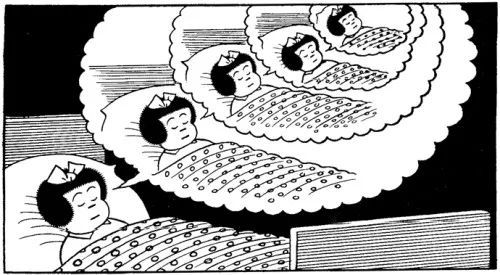
\includegraphics[scale=0.7]{img/Chapter5/5-3/1.png}
\end{figure}

\vspace{0.5cm}

\mybox{讲故事}

\begin{lstlisting}[language=C++]
#include <iostream>
#include <string>

using namespace std;

void tell_story() {
	string story;
	story += "从前有座山,山里有座庙\n";
	story += "庙里有个老和尚\n";
	story += "老和尚在对小和尚讲故事:\n";
	cout << story;

	tell_story();
}

int main() {
	tell_story();
	return 0;
}
\end{lstlisting}

\begin{tcolorbox}
	\mybox{运行结果}
	\begin{verbatim}
从前有座山,山里有座庙
庙里有个老和尚
老和尚在对小和尚讲故事:
从前有座山,山里有座庙
庙里有个老和尚
老和尚在对小和尚讲故事:
从前有座山,山里有座庙
庙里有个老和尚
老和尚在对小和尚讲故事:
...
	\end{verbatim}
\end{tcolorbox}

一个永远无法结束的递归函数最终会导致栈溢出。因此递归函数需要确定一个结束条件,确保在递归过程中能在合适的地方停止并返回。\\

\mybox{阶乘}

\begin{lstlisting}[language=C++]
#include <iostream>

using namespace std;

int factorial(int n) {
	if(n == 0 || n == 1) {
		return 1;
	}
	return n * factorial(n-1);
}

int main() {
	cout << "5! = " << factorial(5) << endl;
	return 0;
}
\end{lstlisting}

\begin{tcolorbox}
	\mybox{运行结果}
	\begin{verbatim}
5! = 120
	\end{verbatim}
\end{tcolorbox}

\begin{figure}[H]
	\centering
	\begin{tikzpicture}[]
		\draw (0,0) rectangle (3,1.5);
		\draw (3,-2) rectangle (6,-0.5);
		\draw (6,-4) rectangle (9,-2.5);
		\draw (9,-6) rectangle (12,-4.5);
		\draw (12,-8) rectangle (15,-6.5);

		\draw (12.75,-10.75) rectangle (14.25,-9.25);
		\draw (9.75,-8.75) rectangle (11.25,-7.25);
		\draw (6.75,-6.75) rectangle (8.25,-5.25);
		\draw (3.75,-4.75) rectangle (5.25,-3.25);
		\draw (0.75,-2.75) rectangle (2.25,-1.25);

		\draw (1.5,0.75) node {$ factorial(5) $};
		\draw (4.5,-1.25) node {$ factorial(4) $};
		\draw (7.5,-3.25) node {$ factorial(3) $};
		\draw (10.5,-5.25) node {$ factorial(2) $};
		\draw (13.5,-7.25) node {$ factorial(1) $};

		\draw (13.5,-10) node {$ 1 $};
		\draw (10.5,-8) node {$ 2 $};
		\draw (7.5,-6) node {$ 6 $};
		\draw (4.5,-4) node {$ 24 $};
		\draw (1.5,-2) node {$ 120 $};

		\draw[->] (3,0.75) -- (4.5,0.75) -- (4.5,-0.5);
		\draw[->] (6,-1.25) -- (7.5,-1.25) -- (7.5,-2.5);
		\draw[->] (9,-3.25) -- (10.5,-3.25) -- (10.5,-4.5);
		\draw[->] (12,-5.25) -- (13.5,-5.25) -- (13.5,-6.5);

		\draw[->] (12.75,-10) -- (10.5,-10) -- (10.5,-8.75);
		\draw[->] (9.75,-8) -- (7.5,-8) -- (7.5,-6.75);
		\draw[->] (6.75,-6) -- (4.5,-6) -- (4.5,-4.75);
		\draw[->] (3.75,-4) -- (1.5,-4) -- (1.5,-2.75);

		\draw (4.5,1) node {$ 5 * factorial(4) $};
		\draw (7.5,-1) node {$ 4 * factorial(3) $};
		\draw (10.5,-3) node {$ 3 * factorial(2) $};
		\draw (13.5,-5) node {$ 2 * factorial(1) $};

		\draw (11,-10.5) node {$ 2 * 1 $};
		\draw (8,-8.5) node {$ 3 * 2 $};
		\draw (5,-6.5) node {$ 4 * 6 $};
		\draw (2,-4.5) node {$ 5 * 24 $};
	\end{tikzpicture}
	\caption{阶乘}
\end{figure}

\vspace{0.5cm}

\mybox{斐波那契数列}

\begin{lstlisting}[language=C++]
#include <iostream>

using namespace std;

int fibonacci(int n) {
	if (n == 1 || n == 2) {
		return n;
	}
	return fibonacci(n - 2) + fibonacci(n - 1);
}

int main() {
	int n = 7;
	cout << fibonacci(n) << endl;
	return 0;
}
\end{lstlisting}

\begin{tcolorbox}
	\mybox{运行结果}
	\begin{verbatim}
21
	\end{verbatim}
\end{tcolorbox}

\begin{figure}[H]
	\centering
	\begin{tikzpicture}[
			level distance=2.4cm,
			level 1/.style={sibling distance=6cm},
			level 2/.style={sibling distance=3cm},
			level 3/.style={sibling distance=2cm}
		]
		\node {$ f(5) $}
		child {
				node {$ f(3) $}
				child {node {$ f(1) $}}
				child {node {$ f(2) $}}
			}
		child {
				node {$ f(4) $}
				child {node {$ f(2) $}}
				child {
						node {$ f(3) $}
						child {node {$ f(1) $}}
						child {node {$ f(2) $}}
					}
			};
	\end{tikzpicture}
	\caption{递归树}
\end{figure}

递归的特点就是将一个复杂的大问题逐步简化为一个可以解决的小问题,然后再逐步计算出大问题的解。\\

递归的优点在于代码简洁易懂,但是缺点也很明显,就是效率很低。每次递归都会产生函数调用,而函数调用的开销是很大的,不适合用来解决大规模的问题。\\

例如在计算斐波那契数列的第40项时,递归需要花费大量时间,因为其中包含了大量的重复计算。相比而言,使用循环的方式能够节省大量的时间。因此像阶乘和斐波那契数列这样的情况,通常会采用循环,而不是递归进行计算。\\

然而还存在很多问题不得不使用递归的思想才能解决。\\

\mybox{阿克曼函数}

\begin{align}\nonumber
	A(m, n) =
	\begin{cases}
		n + 1             & m = 0        \\
		A(m-1, 1)         & m > 0, n = 0 \\
		A(m-1, A(m, n-1)) & m > 0, n > 0 \\
	\end{cases}
\end{align}

\begin{lstlisting}[language=C++]
#include <iostream>

using namespace std;

int A(int m, int n) {
	if (m == 0) {
		return n + 1;
	} else if (m > 0 && n == 0) {
		return A(m - 1, 1);
	} else {
		return A(m - 1, A(m, n - 1));
	}
}

int main() {
	cout << A(3, 4) << endl;
	return 0;
}
\end{lstlisting}

\begin{tcolorbox}
	\mybox{运行结果}
	\begin{verbatim}
125
	\end{verbatim}
\end{tcolorbox}

\vspace{0.5cm}

\mybox{汉诺塔}\\

有三根柱子A、B、C,A柱子上从下到上套有n个圆盘,要求将A柱子上的圆盘移动到C柱子上。每次只能移动一个圆盘,且大圆盘始终不能叠在小圆盘上面。\\

\begin{figure}[H]
	\centering
	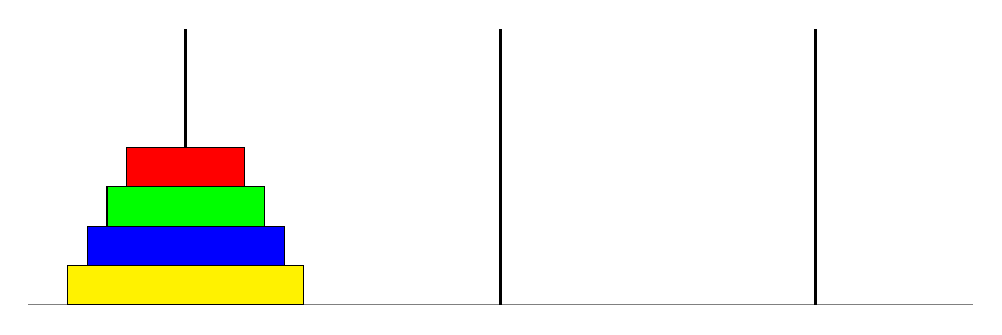
\begin{tikzpicture}[scale=0.5]
		\draw[-, gray] (0,0) -- (24,0);
		\draw[-, very thick] (4,0) -- (4,7);
		\draw[-, very thick] (12,0) -- (12,7);
		\draw[-, very thick] (20,0) -- (20,7);

		\draw[fill=red] (2.5,3) rectangle (5.5,4);
		\draw[fill=green] (2,2) rectangle (6,3);
		\draw[fill=blue] (1.5,1) rectangle (6.5,2);
		\draw[fill=yellow] (1,0) rectangle (7,1);
	\end{tikzpicture}
	\caption{汉诺塔}
\end{figure}

递归算法求解汉诺塔问题:

\begin{enumerate}
	\item 将n-1个圆盘从A借助C移到B。
	\item 将第n个圆盘从A移到C。
	\item 将n-1个圆盘从B借助A移到C。
\end{enumerate}

\vspace{-0.5cm}

\begin{lstlisting}[language=C++]
#include <iostream>

using namespace std;

int moves = 0;

void hanoi(int n, char src, char mid, char dst) {
	if (n == 1) {
		cout << src << " -> " << dst << endl;
		moves++;
	} else {
		// move top n-1 disks from src to mid
		hanoi(n - 1, src, dst, mid);
		cout << src << " -> " << dst << endl;
		moves++;
		// move top n-1 disks from mid to dst
		hanoi(n - 1, mid, src, dst);
	}
}

int main() {
	hanoi(3, 'A', 'B', 'C');
	cout << "Moves: " << moves << endl;
	return 0;
}
\end{lstlisting}

\begin{tcolorbox}
	\mybox{运行结果}
	\begin{verbatim}
A -> C
A -> B
C -> B
A -> C
B -> A
B -> C
A -> C
Moves: 7
	\end{verbatim}
\end{tcolorbox}

假设每次移动花费1秒,解决一个64层的汉诺塔问题大约需要5800亿年。\\

\begin{figure}[H]
	\centering
	
\includegraphics[]{img/Chapter5/5-3/2.png}
\end{figure}

\newpage
\chapter{预处理}

\section{预处理}

\subsection{宏(Macro)}

宏是一种简单的文本替换工具,可以用于定义一个特定的常量或表达式,一般用大写表示。宏定义使用\#define指令,在编译期间,编译器会将程序中所有的宏替换为其内容。\\

与变量的定义不同的是,宏没有类型,也不占内存空间。\\

\mybox{圆}

\begin{lstlisting}[language=C++]
#include <iostream>
#define PI 3.14159

using namespace std;

double perimeter(double r) {
    return 2 * PI * r;
}

double area(double r) {
    return PI * r * r;
}

int main() {
    double radius;
    cout << "Enter radius: ";
    cin >> radius;

    cout << "Perimeter: " << perimeter(radius) << endl;
    cout << "Area: " << area(radius) << endl;

    return 0;
}
\end{lstlisting}

\begin{tcolorbox}
    \mybox{运行结果}
    \begin{verbatim}
Enter radius: 5
Perimeter: 31.42
Area: 78.54
	\end{verbatim}
\end{tcolorbox}

宏也可以像函数一样传递参数,但是宏的参数不会进行类型检查,宏最终同样也会在编译期间被展开。\\

但是由于宏定义的内容在编译时会被替换到代码中,有时候会导致运算的优先级发生改变。

\vspace{-0.5cm}

\begin{lstlisting}[language=C++]
#define SQUARE x * x
\end{lstlisting}

例如SQUARE(2 + 3)会被展开为2 + 3 * 2 + 3,而不是(2 + 3) * (2 + 3)。因此,最好在宏中使用括号来避免这种情况。

\vspace{-0.5cm}

\begin{lstlisting}[language=C++]
#define SQUARE (x * x)
\end{lstlisting}

\vspace{0.5cm}

\subsection{条件编译}

条件编译是一种在编译时根据宏的定义来决定是否编译某段代码的方法。\\

\mybox{斐波那契数列}

\begin{lstlisting}[language=C++]
#include <iostream>

using namespace std;

#define RECURSION

#ifdef RECURSION
int fibonacci(int n) {
    if (n == 0) {
        return 0;
    } else if (n == 1) {
        return 1;
    }
    return fibonacci(n - 1) + fibonacci(n - 2);
}
#else
int fibonacci(int n) {
    int seq[n];
    seq[0] = 0;
    seq[1] = 1;

    for (int i = 2; i <= n; i++) {
        seq[i] = seq[i - 1] + seq[i - 2];
    }

    return seq[n];
}
#endif

int main() {
    int n;
    cout << "Enter n: ";
    cin >> n;
    cout << fibonacci(n) << endl;
    return 0;
}
\end{lstlisting}

\begin{tcolorbox}
    \mybox{运行结果}
    \begin{verbatim}
Enter n: 7
13
	\end{verbatim}
\end{tcolorbox}

\newpage

\section{多文件编译}

\subsection{编译(Compile)}

集成开发环境IDE(Integrated Development Environment)包含了文本编辑器、编译器、调试器和其它工具,可以很方便地进行开发。但是对于大型项目,使用命令行编译更加灵活和高效。\\

\mybox{交换}

\begin{lstlisting}[language=C++]
#include <iostream>

using namespace std;

#define SWAP(a, b) {int t; t = a; a = b; b = t;}

int main() {
    int a = 1;
    int b = 2;

    cout << "Before: a = " << a << ", b = " << b << endl;
    SWAP(a, b);
    cout << "After: a = " << a << ", b = " << b << endl;

    return 0;
}
\end{lstlisting}

\vspace{-0.5cm}

\begin{lstlisting}
g++ -Wall swap.cpp -o swap
./swap
\end{lstlisting}

其中g++表示编译器的名称,-Wall表示要输出所有警告信息,swap.cpp为需编译的源文件,-o用于指定输出的可执行文件的名称为swap。编译成功后使用./swap即可运行。\\

一个完整的编译过程包含4个步骤:

\begin{enumerate}
    \item 预处理:将头文件、宏定义等展开
          \vspace{-0.5cm}
          \begin{lstlisting}
g++ -E swap.cpp -o swap.i
            \end{lstlisting}

    \item 编译:将预处理后的代码转换为汇编代码
          \vspace{-0.5cm}
          \begin{lstlisting}
g++ -S swap.i -o swap.s
            \end{lstlisting}

    \item 汇编:将汇编代码转换为机器码
          \vspace{-0.5cm}
          \begin{lstlisting}
g++ -c swap.s -o swap.o
            \end{lstlisting}

    \item 链接:将目标文件链接为可执行文件
          \vspace{-0.5cm}
          \begin{lstlisting}
g++ swap.o -o swap
            \end{lstlisting}
\end{enumerate}

\vspace{0.5cm}

\subsection{多文件编译}

模块化编程的目的是为了将程序分解成多个独立、可重用的部分。当程序变得复杂时,分成多个文件可以使得程序逻辑更加清晰、易于维护。\\

在多文件中,每个模板一般都分为.h和.cpp两部分,其中.h文件用于声明函数原型,.cpp文件用于实现函数。这样其它文件只需要包含.h文件即可使用这些函数,就像包含头文件iostream一样,只不过自定义的头文件一般使用双引号包含。\\

由于一个头文件可以被多个源文件包含,为了避免重复定义,一般在头文件的开头使用条件编译来判断是否已经被包含。\\

\mybox{面积}

\begin{lstlisting}[language=C, title=geometry.h]
#ifndef _GEOMETRY_H_
#define _GEOMETRY_H_

double circle_area(double radius);

double triangle_area(double base, double height);

#endif
\end{lstlisting}

\begin{lstlisting}[language=C, title=geometry.c]
#include "geometry.h"

#define PI 3.1415926

double circle_area(double radius) {
    return PI * radius * radius;
}

double triangle_area(double base, double height) {
    return base * height / 2;
}
\end{lstlisting}

\begin{lstlisting}[language=C, title=area.c]
#include <stdio.h>
#include "geometry.h"

int main() {
    printf("Area of circle: %.2f\n", circle_area(5));
    printf("Area of triangle: %.2f\n", triangle_area(5, 10));
    return 0;
}
\end{lstlisting}

\vspace{-0.5cm}

\begin{lstlisting}
gcc -Wall geometry.c area.c -o area
./area
\end{lstlisting}

\begin{tcolorbox}
    \mybox{运行结果}
    \begin{verbatim}
Area of circle: 78.54
Area of triangle: 25.00
	\end{verbatim}
\end{tcolorbox}

\newpage
\chapter{指针}

\section{指针}

\subsection{指针(Pointer)}

每个变量都会在内存中占用一定的空间,不同类型的变量占用的空间大小也不同。每个空间都有一个地址,一般采用十六进制表示,如0x0060FEFC。\\

有时候需要通过变量的地址对变量进行操作,这时候就需要将变量的地址保存起来,保存地址的变量就成为指针。

\begin{figure}[H]
    \centering
    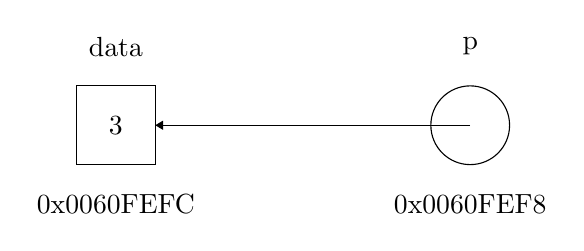
\begin{tikzpicture}
        \draw (0,0) rectangle node{3} (1,1);
        \draw (0.5,1.5) node{data};
        \draw (0.5,-0.5) node{0x0060FEFC};

        \draw (5,0.5) circle (0.5);
        \draw (5,1.5) node{p};
        \draw (5,-0.5) node{0x0060FEF8};

        \draw[->] (5,0.5) -- (1,0.5);
    \end{tikzpicture}
\end{figure}

*用于声明一个指针变量,例如int *p表示p是一个指针,指向一个int类型的变量的地址。通过取地址运算符\&可以获取变量的地址,占位符\%p能够以十六进制的形式输出地址。\\

既然指针保存了另一个变量的地址,那么通过指针就可以访问到那个变量上的数据。在指针变量前使用*运算符,就可以获取到指针所指向的变量的值。

\begin{figure}[H]
    \centering
    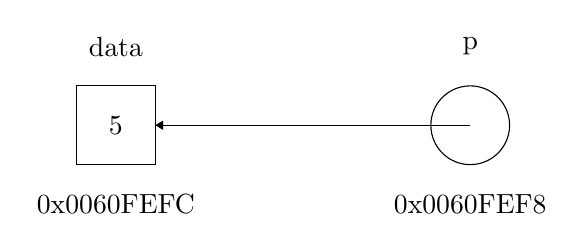
\begin{tikzpicture}
        \draw (0,0) rectangle node{5} (1,1);
        \draw (0.5,1.5) node{data};
        \draw (0.5,-0.5) node{0x0060FEFC};

        \draw (5,0.5) circle (0.5);
        \draw (5,1.5) node{p};
        \draw (5,-0.5) node{0x0060FEF8};

        \draw[->] (5,0.5) -- (1,0.5);
    \end{tikzpicture}
\end{figure}

\mybox{指针}

\begin{lstlisting}[language=C++]
#include <iostream>

using namespace std;

int main() {
    int data = 3;
    int *p = &data;

    cout << "Value of data: " << data << endl;
    cout << "Address of data: " << &data << endl;

    cout << "Value of p: " << p << endl;
    cout << "Address of p: " << &p << endl;
    cout << "Value of data pointed by p: " << *p << endl;
    
    *p = 5;

    cout << "Value of data: " << data << endl;
    cout << "Value of data pointed by p: " << *p << endl;

    return 0;
}
\end{lstlisting}

\begin{tcolorbox}
    \mybox{运行结果}
    \begin{verbatim}
Value of data: 3
Address of data: 0x61fe1c
Value of p: 0x61fe1c
Address of p: 0x61fe10
Value of data pointed by p: 3
Value of data: 5
Value of data pointed by p: 5
	\end{verbatim}
\end{tcolorbox}

为什么不直接修改变量的值,还要多此一举通过指针修改呢?\\

例如需要实现swap()用于交换两个变量的值,由于传递参数是按值传递(pass by value),所以交换的仅仅只是swap()中局部变量的值。\\

这种情况下就需要使用指针,将需要交换的变量的地址传递给swap(),然后在swap()中交换这两个地址上的值。\\

\mybox{交换}

\begin{lstlisting}[language=C++]
#include <iostream>

using namespace std;

void swap(int *data1, int *data2) {
    int temp = *data1;
    *data1 = *data2;
    *data2 = temp;
}

int main() {
    int a = 3;
    int b = 5;

    cout << "Before: a = " << a << ", b = " << b << endl;
    swap(&a, &b);
    cout << "After: a = " << a << ", b = " << b << endl;
    return 0;
}
\end{lstlisting}

\begin{tcolorbox}
    \mybox{运行结果}
    \begin{verbatim}
Before: a = 3, b = 5
After: a = 5, b = 3
	\end{verbatim}
\end{tcolorbox}

函数最多只能返回一个值,但如果需要有多个值需要返回,就可以使用指针将数据带回。\\

\mybox{一元二次方程}

\begin{lstlisting}[language=C++]
#include <iostream>
#include <cmath>
#include <iomanip>

using namespace std;

/**
 * Solve quadratic equation ax^2 + bx + c = 0.
 * @param a coefficient of x^2
 * @param b coefficient of x
 * @param c constant
 * @param x1 pointer to the first root
 * @param x2 pointer to the second root
 * @return true if the equation has real roots, false otherwise.
 */
bool solver(double a, double b, double c, double *x1, double *x2) {
    double delta = b * b - 4 * a * c;
    if (delta < 0) {
        return false;
    }
    *x1 = (-b + sqrt(delta)) / (2 * a);
    *x2 = (-b - sqrt(delta)) / (2 * a);
    return true;
}

int main() {
    double a, b, c;
    double x1, x2;

    cout << "Quadratic equation ax^2 + bx + c = 0" << endl;
    cout << "Enter coefficients a, b, c: ";
    cin >> a >> b >> c;

    if (solver(a, b, c, &x1, &x2)) {
        cout << fixed << setprecision(2) 
             << "x1 = "  << x1 << ", x2 = " << x2 << endl;
    } else {
        cout << "No real roots" << endl;
    }

    return 0;
}
\end{lstlisting}

\begin{tcolorbox}
    \mybox{运行结果}
    \begin{verbatim}
Quadratic equation ax^2 + bx + c = 0
Enter coefficients a, b, c: 1 -9 20
x1 = 5.00, x2 = 4.00
	\end{verbatim}
\end{tcolorbox}

\vspace{0.5cm}

\subsection{NULL}

如果一个变量声明时没有初始化,那么它的值是不确定的。声明指针时如果不对指针进行初始化,那么它就会指向一块不确定的内存地址,这种指针被称为野指针。\\

使用野指针可能会导致程序崩溃,因为它可能指向一个不可访问的内存地址。因此,如果指针没有指向一个确定的内存地址时,应该将其赋值为空指针NULL。

\vspace{-0.5cm}

\begin{lstlisting}[language=C++]
int *p = NULL;
\end{lstlisting}

\newpage

\section{指针与数组}

\subsection{指针与数组}

数组名本质上就是一个指针,它指向数组的首地址。因此在获取数组的地址时,可以不使用\&运算符。\\

\begin{figure}[H]
    \centering
    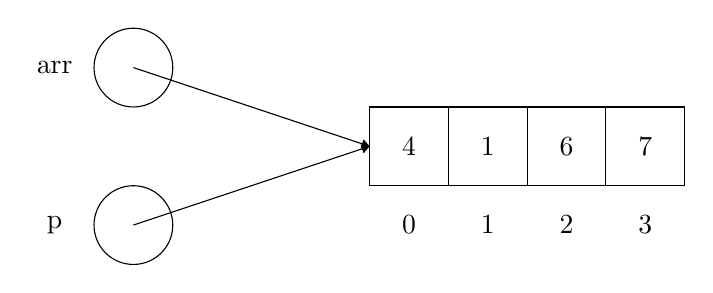
\begin{tikzpicture}
        \draw (0,1) circle (0.5);
        \draw (-1,1) node{arr};

        \draw (0,-1) circle (0.5);
        \draw (-1,-1) node{p};

        \draw (3,-0.5) rectangle (7,0.5);
        \draw (4,-0.5) -- (4,0.5);
        \draw (5,-0.5) -- (5,0.5);
        \draw (6,-0.5) -- (6,0.5);

        \draw (3.5,0) node {4};
        \draw (4.5,0) node {1};
        \draw (5.5,0) node {6};
        \draw (6.5,0) node {7};

        \draw (3.5,-1) node {0};
        \draw (4.5,-1) node {1};
        \draw (5.5,-1) node {2};
        \draw (6.5,-1) node {3};

        \draw[->] (0,1) -- (3,0);
        \draw[->] (0,-1) -- (3,0);
    \end{tikzpicture}
\end{figure}

当对一个指向数组的指针进行加减运算时(如p++和p--),并不是将地址加1或减1,而是根据指针的类型加或减对应字节的长度。例如p是一个int型指针,那么p++会将地址加4(int占4个字节)、p -= 2会将地址减8。\\

\mybox{指针与数组}

\begin{lstlisting}[language=C++]
#include <iostream>

using namespace std;

int main() {
    int arr[] = {4, 1, 6, 7};
    int n = sizeof(arr) / sizeof(arr[0]);
    int *p = arr;

    cout << "Address of arr: " << arr << endl;
    for (int i = 0; i < n; i++) {
        cout << "Address of arr[" << i << "]: " << &arr[i] << endl;
    }

    cout << "Value of p: " << p << endl;
    for (int i = 1; i < n; i++) {
        cout << "Value of p + " << i << ": " << p + i << endl;
    }

    *p = 9;
    *(p + 1) = 8;
    *(p + 2) = 7;
    *(p + 3) = 6;

    for (int i = 0; i < n; i++) {
        cout << "arr[" << i << "]: " << arr[i] << endl;
    }

    return 0;
}
\end{lstlisting}

\begin{tcolorbox}
    \mybox{运行结果}
    \begin{verbatim}
Address of arr: 0x61fdf0   
Address of arr[0]: 0x61fdf0
Address of arr[1]: 0x61fdf4
Address of arr[2]: 0x61fdf8
Address of arr[3]: 0x61fdfc
Value of p: 0x61fdf0
Value of p + 1: 0x61fdf4
Value of p + 2: 0x61fdf8
Value of p + 3: 0x61fdfc
arr[0]: 9
arr[1]: 8
arr[2]: 7
arr[3]: 6
	\end{verbatim}
\end{tcolorbox}

\vspace{0.5cm}

\subsection{数组与函数}

数组作为函数参数时,会将数组的地址传递给函数,函数接收到的是一个指向数组首地址的指针。由于在函数中失去了数组长度的信息,并不能通过sizeof()计算出数组的长度(计算得到的是一个指针变量所占的空间),因此将数组传入函数时,还需要将其长度一并作为参数传给函数。\\

\mybox{查找}

\begin{lstlisting}[language=C++]
#include <iostream>

using namespace std;

int search(int *arr, int n, int key) {
    for (int i = 0; i < n; i++) {
        if (arr[i] == key) {
            return i;
        }
    }
    return -1;
}

int main() {
    int arr[] = {4, 7, 1, 3, 9, 2};
    int n = sizeof(arr) / sizeof(arr[0]);

    int index = search(arr, n, 3);
    if (index == -1) {
        cout << "Not found" << endl;
    } else {
        cout << "Found at index " << index << endl;
    }

    return 0;
}
\end{lstlisting}

\begin{tcolorbox}
    \mybox{运行结果}
    \begin{verbatim}
Found at index 3
	\end{verbatim}
\end{tcolorbox}

\newpage

\section{指针与字符串}

\subsection{指针与字符串}

数组和指针都可以用于定义一个字符串,但是它们内存分配的方式不同,从而导致它们的使用方式也不同。\\

以数组形式定义的字符串,每个字符保存在一个字符数组中。这样的字符串是可以修改的,与普通的数组类似。\\

但是如果让一个指针指向一个字符串,那么这个字符串会被存储在常量区。常量区中的数据是不可以修改的,因此使用指针去修改字符串会导致程序崩溃。\\

\begin{figure}[H]
    \centering
    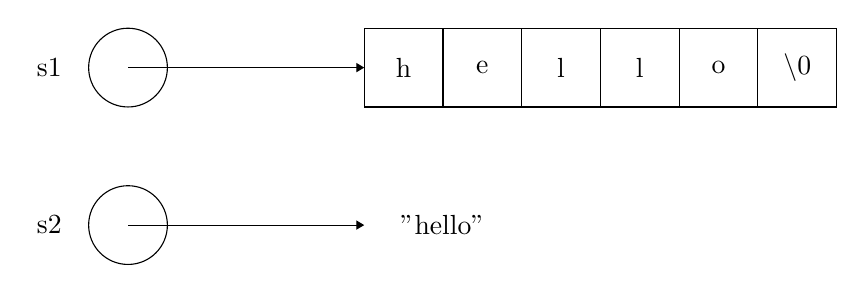
\begin{tikzpicture}
        \draw (0,0) circle (0.5);
        \draw (-1,0) node{s1};

        \draw (3,-0.5) rectangle (9,0.5);
        \draw (4,-0.5) -- (4,0.5);
        \draw (5,-0.5) -- (5,0.5);
        \draw (6,-0.5) -- (6,0.5);
        \draw (7,-0.5) -- (7,0.5);
        \draw (8,-0.5) -- (8,0.5);

        \draw (3.5,0) node {h};
        \draw (4.5,0) node {e};
        \draw (5.5,0) node {l};
        \draw (6.5,0) node {l};
        \draw (7.5,0) node {o};
        \draw (8.5,0) node {$ \backslash $0};

        \draw[->] (0,0) -- (3,0);

        \draw (0,-2) circle (0.5);
        \draw (-1,-2) node{s2};
        \draw (4,-2) node {"hello"};
        \draw[->] (0,-2) -- (3,-2);
    \end{tikzpicture}
\end{figure}

\vspace{-0.5cm}

\begin{lstlisting}[language=C++]
char s1[] = "hello";
s1[0] = 'H';
cout << s1 << endl;

char *s2 = "hello";
s2[0] = 'H';        // error
cout << s2 << endl;
\end{lstlisting}

在对指向字符串的指针进行赋值操作的时候,并不会产生新的字符串,只是让两个指针都指向同一个字符串,对任意一个指针做的操作都会影响另一个指针。\\

\begin{figure}[H]
    \centering
    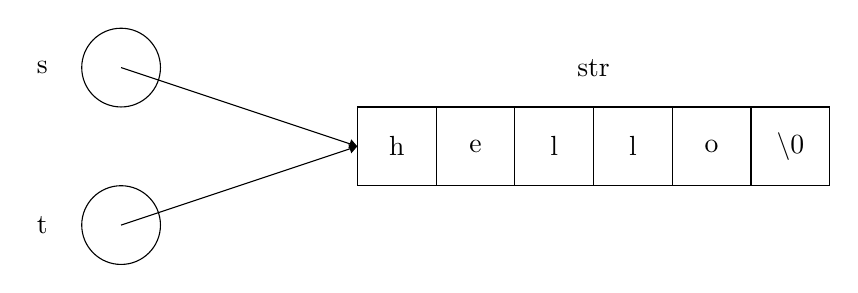
\begin{tikzpicture}
        \draw (0,1) circle (0.5);
        \draw (-1,1) node{s};

        \draw (0,-1) circle (0.5);
        \draw (-1,-1) node{t};

        \draw (3,-0.5) rectangle (9,0.5);
        \draw (4,-0.5) -- (4,0.5);
        \draw (5,-0.5) -- (5,0.5);
        \draw (6,-0.5) -- (6,0.5);
        \draw (7,-0.5) -- (7,0.5);
        \draw (8,-0.5) -- (8,0.5);

        \draw (3.5,0) node {h};
        \draw (4.5,0) node {e};
        \draw (5.5,0) node {l};
        \draw (6.5,0) node {l};
        \draw (7.5,0) node {o};
        \draw (8.5,0) node {$ \backslash $0};
        \draw (6,1) node {str};

        \draw[->] (0,1) -- (3,0);
        \draw[->] (0,-1) -- (3,0);
    \end{tikzpicture}
\end{figure}

\mybox{指向字符串的指针}

\begin{lstlisting}[language=C++]
#include <iostream>

using namespace std;

int main() {
    char str[] = "hello";
    char *s = str;
    char *t = s;

    s[0] = 'H';
    cout << "s = " << s << endl;
    cout << "t = " << t << endl;

    return 0;
}
\end{lstlisting}

\begin{tcolorbox}
    \mybox{运行结果}
    \begin{verbatim}
s = Hello
t = Hello
	\end{verbatim}
\end{tcolorbox}

\newpage

\section{二级指针}

\subsection{二级指针(Pointer to pointer)}

既然指针也是一个变量,那么一个指针也可以指向另一个指针,这样的指针称为二级指针。

\begin{figure}[H]
    \centering
    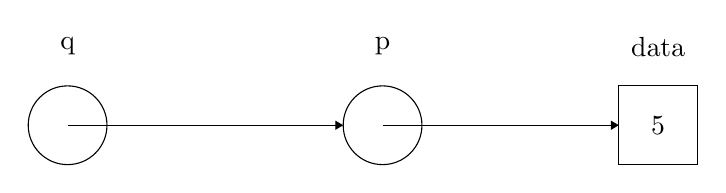
\begin{tikzpicture}
        \draw (0,0) circle (0.5);
        \draw (0,1) node{q};
        \draw (4,0) circle (0.5);
        \draw (4,1) node{p};

        \draw (7,-0.5) rectangle (8,0.5);
        \draw (7.5,0) node {5};
        \draw (7.5,1) node {data};

        \draw[->] (0,0) -- (3.5,0);
        \draw[->] (4,0) -- (7,0);
    \end{tikzpicture}
\end{figure}

其中p是一个int型的指针(int *),指向了data;q是一个指向int型指针的指针(int **),即q指向了一个指向int的指针。\\

\mybox{二级指针}

\begin{lstlisting}[language=C++]
#include <iostream>

using namespace std;

int main() {
    int data = 5;
    int *p = &data;
    int **q = &p;

    cout << "data = " << data << endl;
    cout << "*p = " << *p << endl;
    cout << "**q = " << **q << endl;

    cout << "Address of data = " << &data << endl;
    cout << "Address of p = " << &p << endl;
    cout << "Address of q = " << &q << endl;

    cout << "Value of p = " << p << endl;
    cout << "Value of q = " << q << endl;

    return 0;
}
\end{lstlisting}

\begin{tcolorbox}
    \mybox{运行结果}
    \begin{verbatim}
data = 5
*p = 5  
**q = 5
Address of data = 0x61fe1c
Address of p = 0x61fe10
Address of q = 0x61fe08
Value of p = 0x61fe1c
Value of q = 0x61fe10
	\end{verbatim}
\end{tcolorbox}

\vspace{0.5cm}

\subsection{指针与二维数组}

二级指针还可以用于表示二维数组。与一维数组类似,可以使用下标或*运算符来访问二维数组中的元素。\\

\begin{figure}[H]
    \centering
    \begin{tikzpicture}
        \draw (0,1.5) circle (0.5);
        \draw (0,2.5) node{arr};
        \draw (4,1.5) circle (0.5);

        \draw (7,-2) rectangle (11,2);
        \draw (8,-2) -- (8,2);
        \draw (9,-2) -- (9,2);
        \draw (10,-2) -- (10,2);
        \draw (7,-1) -- (11,-1);
        \draw (7,0) -- (11,0);
        \draw (7,1) -- (11,1);

        \draw[->] (0,1.5) -- (3.5,1.5);
        \draw[->] (4,1.5) -- (7,1.5);
    \end{tikzpicture}
\end{figure}

例如,arr[2][1]也可以写成*(*(arr + 2) + 1)。

\begin{figure}[H]
    \centering
    \begin{tikzpicture}
        \draw (0,1.5) circle (0.5);
        \draw (0,2.5) node{arr};
        \draw (4,1.5) circle (0.5);

        \draw (7,-2) rectangle (11,2);
        \draw (8,-2) -- (8,2);
        \draw (9,-2) -- (9,2);
        \draw (10,-2) -- (10,2);
        \draw (7,-1) -- (11,-1);
        \draw (7,0) -- (11,0);
        \draw (7,1) -- (11,1);

        \draw[->] (0,1.5) -- (3.5,1.5);
        \draw[->] (4,1.5) -- (8.5,-0.5);
    \end{tikzpicture}
\end{figure}

当如果命令行运行时,可以向main()函数传递命令行参数。传递参数的数量和值可以通过argc(argument count)和argv(argument vector)来获取。argv为一个二维数组,每个元素都是一个字符串,其中argv[0]为当前程序的名称。\\

\mybox{命令行参数}

\begin{lstlisting}[language=C++]
#include <iostream>
#include <cctype>
#include <cstring>

using namespace std;

char *lower(char *s) {
    char *p = s;
    while (*p) {
        *p = tolower(*p);
        p++;
    }
    return s;
}

char *upper(char *s) {
    char *p = s;
    while (*p) {
        *p = toupper(*p);
        p++;
    }
    return s;
}

void usage(const char *program) {
    cout << "Usage: " << program << " [option] [string]" << endl;
    cout << "--lower: convert string to lower case" << endl;
    cout << "--upper: convert string to upper case" << endl;
}

int main(int argc, char **argv) {
    if (argc != 3) {
        usage(argv[0]);
        return 1;
    }

    char *option = argv[1];
    char *string = argv[2];

    if (strcmp(option, "--lower") == 0) {
        cout << "Lower: " << lower(string) << endl;
    } else if (strcmp(option, "--upper") == 0) {
        cout << "Upper: " << upper(string) << endl;
    } else {
        usage(argv[0]);
        return 1;
    }

    return 0;
}
\end{lstlisting}

\begin{lstlisting}
g++ -Wall command_line.cpp -o command_line
./command_line --upper "Hello World!"
\end{lstlisting}

\begin{tcolorbox}
    \mybox{运行结果}
    \begin{verbatim}
Upper: HELLO WORLD!
	\end{verbatim}
\end{tcolorbox}

\newpage

\section{引用}

\subsection{引用(Reference)}

引用可以看作是变量的别名,对引用的操作与对变量的操作完全一样。因此引用可以用于传递参数和返回值,避免了复制较大变量的开销。\\

声明引用时必须对其初始化,并且之后不能再将该引用作为其它变量的别名。\\

\mybox{交换}

\begin{lstlisting}[language=C++]
#include <iostream>

using namespace std;

void swap(int &data1, int &data2) {
    int temp = data1;
    data1 = data2;
    data2 = temp;
}

int main() {
    int a = 3;
    int b = 5;

    cout << "Before: a = " << a << ", b = " << b << endl;
    swap(a, b);
    cout << "After: a = " << a << ", b = " << b << endl;
    return 0;
}
\end{lstlisting}

\begin{tcolorbox}
    \mybox{运行结果}
    \begin{verbatim}
Before: a = 3, b = 5
After: a = 5, b = 3
	\end{verbatim}
\end{tcolorbox}

\vspace{0.5cm}

\begin{table}[H]
    \centering
    \setlength{\tabcolsep}{5mm}{
        \begin{tabular}{|c|c|c|}
            \hline
                                  & \textbf{指针}         & \textbf{引用}    \\
            \hline
            \textbf{内存}         & 占用空间              & 不占用空间       \\
            \hline
            \textbf{大小}         & 4字节/8字节           & 被引用对象的大小 \\
            \hline
            \textbf{能否为空}     & 可以为NULL            & 引用对象必须存在 \\
            \hline
            \textbf{能否改变指向} & 可以                  & 不可以           \\
            \hline
            \textbf{使用}         & 通过*对指向的变量操作 & 直接对变量操作   \\
            \hline
            \textbf{层级}         & 可以有多级指针        & 只有一级         \\
            \hline
        \end{tabular}
    }
    \caption{指针与引用的区别}
\end{table}

\newpage

\section{动态内存申请}

\subsection{内存管理}

计算机的内存主要包括:

\begin{enumerate}
    \item 代码区:存储程序执行时使用的指令。
    \item 数据区:存储程序运行时使用的全局变量和静态变量。
    \item 栈区(stack):存储函数调用时使用的局部变量,栈中的内存由编译器自动分配和释放。
    \item 堆区(heap):存储动态分配内存的变量,需要由程序员自己分配和释放。
\end{enumerate}

\begin{figure}[H]
    \centering
    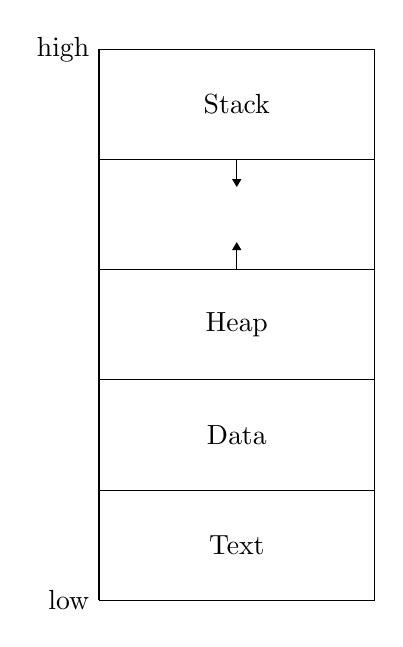
\begin{tikzpicture}[scale=0.7]
        \draw[-] (0,0) -- (0,10) -- (5,10) -- (5,0) -- (0,0);
        \draw[-] (0,2) -- (5,2);
        \draw[-] (0,4) -- (5,4);
        \draw[-] (0,6) -- (5,6);
        \draw[-] (0,8) -- (5,8);

        \draw (0,0) node[left] {low};
        \draw (0,10) node[left] {high};

        \draw (2.5,1) node {Text};
        \draw (2.5,3) node {Data};
        \draw (2.5,5) node {Heap};
        \draw (2.5,9) node {Stack};

        \draw[->] (2.5,8) -- (2.5,7.5);
        \draw[->] (2.5,6) -- (2.5,6.5);
    \end{tikzpicture}
    \caption{内存区域}
\end{figure}

有时候需要在函数中生成一个数组,并且将数组返回给调用者。但是在函数内定义的数组是局部变量,存储于栈区。函数执行完毕后,数组所占用的内存空间会被释放。因此被返回的数组的指针指向的是一个已经被释放的内存空间,这样就会导致程序崩溃。\\

另一种情况是,由于数组一旦声明后,其容量就不能再改变。当需要在运行时动态改变数组容量时,就可以采用动态内存申请的方式。\\

\subsection{malloc()}

malloc()函数定义在<cstdlib>中,用于在堆区申请一块内存空间,其函数原型为:

\vspace{-0.5cm}

\begin{lstlisting}[language=C++]
void* malloc(size_t size);
\end{lstlisting}

malloc()接受一个参数size,表示申请空间的大小(单位:字节),并返回指向申请到的空间的首地址的指针。如果申请失败,则返回NULL。\\

malloc()返回的是无类型指针void *,这是由于malloc()只负责申请指定大小的空间,并不关心这块空间将会被存放什么类型的数据。因此,开发者需要自行将其转换为对应的类型。\\

\mybox{内存}

\begin{lstlisting}[language=C++]
#include <iostream>
#include <cstdlib>

using namespace std;

int main() {
    void *p;
    int cnt = 0;

    // allocate 100MB memory each time
    while ((p = malloc(100 * 1024 * 1024))) {
        cnt++;
    }
    cout << "Allocated " << cnt * 100 << " MB memory" << endl;

    return 0;
}
\end{lstlisting}

\begin{tcolorbox}
    \mybox{运行结果}
    \begin{verbatim}
Allocated 57700 MB memory
	\end{verbatim}
\end{tcolorbox}

\vspace{0.5cm}

\subsection{free()}

通过动态申请来的内存空间需要是需要归还给操作系统,因此需要程序员自行在不需要使用时将其释放。如果不释放内存,这些动态申请的内存空间就会一直占用着,直到程序结束统一被操作系统释放。\\

不释放内存会导致内存泄漏(memory leak),如果一直分配内存而不是释放,最终将会耗尽所有可用的内存,导致程序运行变慢或者崩溃。\\

free()函数用于释放动态申请的内存空间,其接受一个参数ptr,表示要释放的内存空间的首地址。其函数原型为:

\vspace{-0.5cm}

\begin{lstlisting}[language=C++]
void free(void *ptr);
\end{lstlisting}

\vspace{0.5cm}

\mybox{斐波那契数列}

\begin{lstlisting}[language=C++]
#include <iostream>
#include <cstdlib>

using namespace std;

int *generate_fibonacci(int n) {
    int *arr = (int *)malloc(n * sizeof(int));
    if (!arr) {
        return NULL;
    }

    arr[0] = 1;
    arr[1] = 1;
    for (int i = 2; i < n; i++) {
        arr[i] = arr[i - 1] + arr[i - 2];
    }
    return arr;
}

int main() {
    int n = 10;
    int *arr = generate_fibonacci(n);

    for (int i = 0; i < n; i++) {
        cout << arr[i] << " ";
    }
    cout << endl;

    free(arr);
    return 0;
}
\end{lstlisting}

\begin{tcolorbox}
    \mybox{运行结果}
    \begin{verbatim}
1 1 2 3 5 8 13 21 34 55
	\end{verbatim}
\end{tcolorbox}

\vspace{0.5cm}

\subsection{calloc()}

calloc()与malloc()功能类似,也是用于动态申请内存空间的。只是malloc()只接受一个参数作为申请空间的大小,申请到的空间并不会进行初始化;而calloc()接受两个参数,可以申请多个指定大小的空间,并将这些空间初始化为0。calloc()的函数原型为:

\vspace{-0.5cm}

\begin{lstlisting}[language=C++]
void *calloc(size_t nitems, size_t size);
\end{lstlisting}

例如需要申请一个长度为n的int数组,并将其初始化为0:

\vspace{-0.5cm}

\begin{lstlisting}[language=C++]
int *arr = (int *)calloc(n, sizeof(int));
\end{lstlisting}

\vspace{0.5cm}

\subsection{realloc()}

realloc()用于对已经动态申请的内存空间进行重新分配(扩容/缩小),其函数原型为:

\vspace{-0.5cm}

\begin{lstlisting}[language=C++]
void *realloc(void *ptr, size_t size);
\end{lstlisting}

realloc()接受两个参数,第一个参数ptr指向需要重新分配内存空间,第二个参数size表示重新分配空间的大小(单位:字节)。realloc()会将原来内存块中的数据复制到新分配的内存块中,并返回指向新内存块的指针。如果重新分配失败,则返回NULL。\\

\mybox{strip}

\begin{lstlisting}[language=C++]
#include <iostream>
#include <cstdlib>
#include <cstring>
#include <cctype>

using namespace std;

char *strip(char *str) {
    int i = 0;
    int j = strlen(str) - 1;

    while (isspace(str[i]) && str[i] != '\0') {
        i++;
    }

    while (isspace(str[j]) && j >= 0) {
        j--;
    }

    int k = 0;
    while (i <= j) {
        str[k++] = str[i++];
    }
    str[k] = '\0';

    str = (char *)realloc(str, (k + 1) * sizeof(char));
    return str;
}

int main() {
    int len = 32;
    char *str = (char *)calloc(len + 1, sizeof(char));

    strcpy(str, "     Hello World! \n\t ");
    cout << "Before: [" << str << "]" << endl;

    str = strip(str);

    cout << "After: [" << str << "]" << endl;

    free(str);
    return 0;
}
\end{lstlisting}

\begin{tcolorbox}
    \mybox{运行结果}
    \begin{verbatim}
Before: [     Hello World! 
     ]
After: [Hello World!]
	\end{verbatim}
\end{tcolorbox}

\newpage
% \chapter{文件}

\section{文件}

\subsection{fopen()}

文件是存储数据的一种常用方式,程序可以从文件中读取和写入数据,从而实现对数据的持久化存储。\\

在对文件进行操作之前,首先需要使用fopen()函数打开文件,fopen()的函数原型为:

\vspace{-0.5cm}

\begin{lstlisting}[language=C++]
FILE *fopen(const char *filename, const char *mode);
\end{lstlisting}

fopen()接受两个参数,第一个参数是要打开的文件名,第二个参数为打开方式。fopen()会返回一个FILE类型的指针,通过该指针可以对文件进行操作;如果文件打开失败,则返回NULL。\\

\begin{table}[H]
    \centering
    \setlength{\tabcolsep}{5mm}{
        \begin{tabular}{|c|l|}
            \hline
            \textbf{打开方式} & \textbf{功能}                                      \\
            \hline
            r                 & 只读,文件必须存在,否则打开失败                   \\
            \hline
            w                 & 只写,创建一个新文件                               \\
            \hline
            a                 & 追加,如果文件不存在则创建;存在则将数据追加到末尾 \\
            \hline
            r+                & 以r模式打开文件,附带写的功能                      \\
            \hline
            w+                & 以w模式打开文件,附带读的功能                      \\
            \hline
            a+                & 以a模式打开文件,附带读的功能                      \\
            \hline
        \end{tabular}
    }
    \caption{文件打开方式}
\end{table}

\vspace{0.5cm}

\subsection{fclose()}

在对文件操作结束后,需要使用fclose()函数将文件关闭。fclose()函数原型:

\vspace{-0.5cm}

\begin{lstlisting}[language=C++]
int fclose(FILE *stream);
\end{lstlisting}

\vspace{0.5cm}

\mybox{文件}

\begin{lstlisting}[title=data.txt]
This is a test.
\end{lstlisting}

\begin{lstlisting}[language=C++]
#include <iostream>
#include <cstdlib>

using namespace std;

int main() {
    FILE *fp = fopen("data.txt", "r");
    if(!fp) {
        exit(1);
    }
    fclose(fp);
    return 0;
}
\end{lstlisting}

\newpage

\section{文件I/O}

\subsection{fprintf()}

fprintf()函数用于将数据输出到文件中,使用方法与printf()类似。fprintf()的函数原型为:

\vspace{-0.5cm}

\begin{lstlisting}[language=C++]
int fprintf(FILE *stream, const char *format, ...);
\end{lstlisting}

\vspace{0.5cm}

\mybox{成绩}

\begin{lstlisting}[language=C++]
#include <iostream>
#include <cstdlib>

using namespace std;

int main() {
    FILE *fp = fopen("data1.txt", "w");
    int n;
    cout << "Enter number of students: ";
    cin >> n;

    char id[8];
    double score;
    for (int i = 0; i < n; i++) {
        cout << "Enter student " << i + 1 << "'s ID: ";
        cin >> id;
        cout << "Enter student " << i + 1 << "'s score: ";
        cin >> score;
        fprintf(fp, "ID=%s\tScore=%.2f\n", id, score);
    }

    fclose(fp);
    return 0;
}
\end{lstlisting}

\begin{tcolorbox}
    \mybox{运行结果}
    \begin{verbatim}
Enter number of students: 5
Enter student 1's ID: A001
Enter student 1's score: 92
Enter student 2's ID: A002
Enter student 2's score: 73
Enter student 3's ID: A003
Enter student 3's score: 89
Enter student 4's ID: A004
Enter student 4's score: 97
Enter student 5's ID: A005
Enter student 5's score: 65
	\end{verbatim}
\end{tcolorbox}

\begin{tcolorbox}
    \mybox{运行结果}
    \textbf{data1.txt}
    \begin{verbatim}
ID=A001	Score=92.00
ID=A002	Score=73.00
ID=A003	Score=89.00
ID=A004	Score=97.00
ID=A005	Score=65.00
	\end{verbatim}
\end{tcolorbox}

为了统一对各种硬件的操作,不同的硬件设备也都被看作是文件进行管理。计算机中标准输入(stdin)是键盘、标准输出(stdout)是显示器、标准错误(stderr)是显示器。\\

因此,当使用printf()函数时,其实是从将数据输出到显示器上。printf()函数是通过调用fprintf(stdout, ...)来实现的。\\

当需要输出一些错误信息时,可以通过fprintf(stderr, ...)将错误信息输出到标准错误stderr上,这样可以避免将错误信息混入到正常的输出信息中,方便查看和分析。\\

\subsection{fscanf()}

fscanf()函数用于从文件中读取数据,使用方法与scanf()类似。fscanf()的函数原型为:

\vspace{-0.5cm}

\begin{lstlisting}[language=C++]
int fscanf(FILE *stream, const char *format, ...);
\end{lstlisting}

fscanf()函数读取成功时返回实际读取的数据个数,失败时返回文件末尾标志EOF(End of File)。\\

\mybox{平均分}

\begin{lstlisting}[language=C++]
#include <iostream>
#include <cstdlib>
#include <iomanip>

using namespace std;

int main() {
    FILE *fp = fopen("data1.txt", "r");
    if (!fp) {
        cerr << "File open failed." << endl;
        exit(1);
    }

    char id[8];
    double score;
    double sum = 0;
    int n = 0;

    while (fscanf(fp, "ID=%s\tScore=%lf\n", id, &score) != EOF) {
        sum += score;
        n++;
    }
    cout << "Average = "
         << fixed << setprecision(2) << sum / n << endl;

    fclose(fp);
    return 0;
}
\end{lstlisting}

\begin{tcolorbox}
    \mybox{运行结果}
    \begin{verbatim}
Average = 83.20
	\end{verbatim}
\end{tcolorbox}

当使用scanf()函数时,其实是从键盘上读取数据的,scanf()函数是通过调用fscanf(stdin, ...)来实现的。\\

\subsection{fputc()}

fputc()函数用于将一个字符写入文件中,其函数原型为:

\vspace{-0.5cm}

\begin{lstlisting}[language=C++]
int fputc(int ch, FILE *stream);
\end{lstlisting}

fputc()接受两个参数,第一个参数为要写入的字符(ASCII码),第二个参数为文件指针。\\

当向屏幕输出一个字符时,fputc(stdout)等价于putchar()。\\

\mybox{大写字母}

\begin{lstlisting}[language=C++]
#include <iostream>
#include <cstdlib>

using namespace std;

int main() {
    FILE *fp = fopen("data2.txt", "w");

    for (int i = 0; i < 26; i++) {
        fputc('A' + i, fp);
    }

    fclose(fp);
    return 0;
}
\end{lstlisting}

\begin{tcolorbox}
    \mybox{运行结果}
    \textbf{data2.txt}
    \begin{verbatim}
ABCDEFGHIJKLMNOPQRSTUVWXYZ
	\end{verbatim}
\end{tcolorbox}

\vspace{0.5cm}

\subsection{fgetc()}

fgetc()函数用于从文件中读取一个字符,读取成功返回字符的ASCII码,失败返回EOF。fgetc()的函数原型为:

\vspace{-0.5cm}

\begin{lstlisting}[language=C++]
int fgetc(FILE *stream);
\end{lstlisting}

当从键盘读取一个字符时,fgetc(stdin)等价于getchar()。\\

在读取文件时,除了可以通过返回值EOF来判断是否读取到文件末尾外,还可以使用feof()函数,当读到文件末尾时返回非0值,否则返回0。feof()的函数原型为:

\vspace{-0.5cm}

\begin{lstlisting}[language=C++]
int feof(FILE *stream);
\end{lstlisting}

\vspace{0.5cm}

\mybox{源代码统计}

\begin{lstlisting}[language=C++]
#include <iostream>
#include <cstdlib>

using namespace std;

int main() {
    FILE *fp = fopen("statistics.cpp", "r");
    if (!fp) {
        cerr << "File open failed." << endl;
        exit(1);
    }

    int chars = 0;
    int lines = 0;

    while (!feof(fp)) {
        char c = fgetc(fp);
        if (c == '\n') {
            lines++;
        } else {
            chars++;
        }
    }

    cout << "Characters: " << chars << endl;
    cout << "Lines: " << lines << endl;

    fclose(fp);
    return 0;
}
\end{lstlisting}

\begin{tcolorbox}
    \mybox{运行结果}
    \begin{verbatim}
Characters: 485
Lines: 29
	\end{verbatim}
\end{tcolorbox}

\vspace{0.5cm}

\subsection{fputs()}

fputs()函数用于将一个字符串写入文件,其函数原型为:

\vspace{-0.5cm}

\begin{lstlisting}[language=C++]
int fputs(const char *str, FILE *stream);
\end{lstlisting}

当向屏幕输出一个字符串时,fputs(stdout)等价于puts()。\\

\mybox{Computer Science Quotes}

\begin{lstlisting}[language=C++]
#include <iostream>
#include <cstdlib>

using namespace std;

int main() {
    const char *quotes[] = {
        "Talk is cheap. Show me the code.",
        "Code never lies, comments sometimes do.",
        "Stay Hungry Stay Foolish.",
    };
    int n = sizeof(quotes) / sizeof(quotes[0]);

    FILE *fp = fopen("data3.txt", "w");

    for (int i = 0; i < n; i++) {
        fputs(quotes[i], fp);
        fputc('\n', fp);
    }

    fclose(fp);
    return 0;
}
\end{lstlisting}

\begin{tcolorbox}
    \mybox{运行结果}
    \textbf{data3.txt}
    \begin{verbatim}
Talk is cheap. Show me the code.
Code never lies, comments sometimes do.
Stay Hungry Stay Foolish.
	\end{verbatim}
\end{tcolorbox}

\vspace{0.5cm}

\subsection{fgets()}

fgets()函数用于从文件读取一行数据,读取成功返回指向字符串的指针,失败则返回NULL。fgets()的函数原型为:

\vspace{-0.5cm}

\begin{lstlisting}[language=C++]
char *fgets(char *str, int n, FILE *stream);
\end{lstlisting}

fgets()接受三个参数,第一个参数用于保存读取到的字符串,第二个参数用于指定读取的最大字符数(包括结尾的$ \backslash $0),第三个参数为文件指针。\\

\mybox{解析单词}

\begin{lstlisting}[language=C++]
#include <stdio.h>
#include <stdlib.h>
#include <string.h>
#include <ctype.h>

int main() {
    FILE *fp = fopen("data3.txt", "r");
    if (!fp) {
        fprintf(stderr, "File open failed.\n");
    }

    char line[128];
    while (fgets(line, sizeof(line), fp) != NULL) {
        char *token = strtok(line, " \t\n");
        while (token != NULL) {
            // remove punctuations
            int i = strlen(token) - 1;
            while (!isalpha(token[i])) {
                i--;
            }
            token[i + 1] = '\0';

            printf("%s\n", token);
            token = strtok(NULL, " \t\n");
        }
    }

    fclose(fp);
    return 0;
}
\end{lstlisting}

\begin{tcolorbox}
    \mybox{运行结果}
    \begin{verbatim}
Talk
is
cheap
Show
me
the
code
Code
never
lies
comments
sometimes
do
Stay
Hungry
Stay
Foolish
	\end{verbatim}
\end{tcolorbox}

\newpage
% \chapter{结构体}

\section{枚举}

\subsection{枚举(Enumeration)}

枚举类型可以将一组相关的常量定义为一个类型,并为这些常量赋予一个可读性较高的名字。枚举类型在定义之后就可以像宏常量一样去使用。\\

例如需要定义一个星期:

\vspace{-0.5cm}

\begin{lstlisting}[language=C]
enum Weekday {
    SUN, MON, TUE, WED, THU, FRI, SAT
};
\end{lstlisting}

枚举值默认从0开始,因此SUN的值为0、MON的值为1、TUE的值为2,以此类推。\\

当需要指定枚举值时,可以直接在某个枚举常量后赋值,之后的枚举常量的值会在此基础上依次加1。\\

例如需要定义月份:

\vspace{-0.5cm}

\begin{lstlisting}[language=C]
enum Month {
    JAN = 1, FEB, MAR, APR, MAY, JUN,
    JUL, AUG, SEP, OCT, NOV, DEC,
};
\end{lstlisting}

\newpage

\section{联合体}

\subsection{联合体(Union)}

联合体允许在同一个内存位置存储不同类型的数据,联合体中多个变量共享同一块内存空间,因此联合体所占空间取决于占用空间最大的成员。这意味着在任意时刻,联合体的内存只能用于存储单个成员,这样可以有效节省内存。\\

\mybox{联合体}

\begin{lstlisting}[language=C]
#include <stdio.h>

union Value {
    int int_data;
    char char_data;
};

int main() {
    union Value val;

    val.char_data = 'A';
    printf("val.int_data = %d\n", val.int_data);

    val.int_data = 97;
    printf("val.char_data = %c\n", val.char_data);

    return 0;
}
\end{lstlisting}

\begin{tcolorbox}
    \mybox{运行结果}
    \begin{verbatim}
val.int_data = 65
val.char_data = a
	\end{verbatim}
\end{tcolorbox}

\newpage

\section{结构体}

\subsection{结构体(Structure)}

与联合体不同,结构体的成员在内存中占用不同的空间,因此结构体所占空间是所有成员占用空间的总和。\\

结构体通常用于存储复杂的数据类型,将一些相关的变量组合在一起。例如:

\begin{itemize}
    \item 日期(年、月、日)
          \vspace{-0.5cm}
          \begin{lstlisting}[language=C]
struct Date {
    int year;
    int month;
    int day;
};
    \end{lstlisting}

    \item 坐标(横坐标、纵坐标)
          \vspace{-0.5cm}
          \begin{lstlisting}[language=C]
struct Coordinate {
    double x;
    double y;
};
    \end{lstlisting}

    \item 学生信息(姓名、出生日期、成绩)
          \vspace{-0.5cm}
          \begin{lstlisting}[language=C]
struct Student {
    char name[32];
    struct Date date_of_birth;
    double score;
};
    \end{lstlisting}
\end{itemize}

\vspace{0.5cm}

\subsection{typedef}

typedef用于给数据类型定义别名,通过使用typedef可以简化结构体的声明,不用每次都加上struct关键字了。

\vspace{-0.5cm}
\begin{lstlisting}[language=C]
typedef struct  {
    int year;
    int month;
    int day;
} Date;

typedef struct {
    char name[32];
    Date date_of_birth;
    double score;
} Student;
\end{lstlisting}

\vspace{0.5cm}

\subsection{结构体指针}

当结构体变量作为函数参数传递时,如果结构体变量很大,那么会消耗大量时间将结构体变量复制到函数的参数中。\\

为了避免这种情况,可以使用结构体指针作为函数参数,这样只需要将结构体变量的地址传递给函数,函数内部就可以直接访问结构体变量了。\\

使用->运算符可以访问结构体指针所指的结构变量中的成员。\\

\mybox{倒数}

\begin{lstlisting}[language=C]
#include <stdio.h>
#include <stdlib.h>

typedef struct {
    int numerator;
    int denominator;
} Fraction;

void reciprocal(Fraction *f) {
    if (f->numerator == 0) {
        fprintf(stderr, "Error: Denominator cannot be zero.\n");
        exit(1);
    } else {
        int temp = f->numerator;
        f->numerator = f->denominator;
        f->denominator = temp;
    }
}

int main() {
    Fraction fraction = {2, 5};  // 2/5

    printf("Reciprocal of ");
    printf("%d/%d is ", fraction.numerator, fraction.denominator);
    reciprocal(&fraction);
    printf("%d/%d\n", fraction.numerator, fraction.denominator);

    return 0;
}
\end{lstlisting}

\begin{tcolorbox}
    \mybox{运行结果}
    \begin{verbatim}
Reciprocal of 2/5 is 5/2
	\end{verbatim}
\end{tcolorbox}

\newpage
% \chapter{C++基础}

\section{重载函数}

\subsection{函数默认参数}

在进行函数参数定义的时候,也可以设置默认值。当参数没有传递的时候就利用默认值来进行参数内容的填充,如果在参数上定义了默认值,那么该参数一定要放在参数列表的最后。\\

\mybox{函数默认参数}

\begin{lstlisting}[language=C++]
#include <iostream>

using namespace std;

void setDate(int year = 1970, int month = 1, int day = 1) {
    cout << year << "/" << month << "/" << day << endl;
}

int main() {
    setDate(2021, 8, 15);
    setDate(2021, 7);
    setDate(2021);
    setDate();
    return 0;
}
\end{lstlisting}

\begin{tcolorbox}
	\mybox{运行结果}
	\begin{verbatim}
2021/8/15
2021/7/1
2021/1/1
1970/1/1
	\end{verbatim}
\end{tcolorbox}

\vspace{0.5cm}

\subsection{重载函数}

重载(overload)表示在同一个作用域中声明了一个与之前声明过的函数具有相同名称的函数,但是它们的参数列表不同。当调用一个重载函数时,编译器通过传递的参数类型,选用最合适的定义。\\

\mybox{重载函数}

\begin{lstlisting}[language=C++]
#include <iostream>
using namespace std;

int max(int num1, int num2) {
    return num1 > num2 ? num1 : num2;
}

double max(double num1, double num2) {
    return num1 > num2 ? num1 : num2;
}

char max(char num1, char num2) {
    return num1 > num2 ? num1 : num2;
}

int main() {
    cout << max(2, 8) << endl;
    cout << max(3.14, 2.71) << endl;
    cout << max('H', 'D') << endl;
    return 0;
}
\end{lstlisting}

\begin{tcolorbox}
	\mybox{运行结果}
	\begin{verbatim}
8
3.14
H
	\end{verbatim}
\end{tcolorbox}

\subsection{new/delete}

new和delete运算符用于动态申请和释放内存空间。如果空间分配失败,程序则抛出bad\_alloc异常。

\vspace{-0.5cm}

\begin{lstlisting}[language=C++]
int *p = new int;
int *q = new int[N];

delete p;
delete[] q;
\end{lstlisting}

\vspace{0.5cm}

\begin{table}[H]
    \centering
    \setlength{\tabcolsep}{5mm}{
        \begin{tabular}{|c|c|c|}
            \hline
                              & \textbf{new/delete}      & \textbf{malloc()/free()} \\
            \hline
            \textbf{类型}     & 运算符                   & 函数                     \\
            \hline
            \textbf{分配方式} & 根据数据类型             & 根据指定大小             \\
            \hline
            \textbf{返回值}   & 返回所分配数据类型的指针 & 返回void *               \\
            \hline
            \textbf{分配失败} & 抛出bad\_alloc异常       & 返回NULL                 \\
            \hline
        \end{tabular}
    }
    \caption{new/delete与malloc()/free()的区别}
\end{table}

\newpage
% \chapter{封装}

\section{类与对象}

\subsection{类与对象}

类(class)表示同一类具有相同特征和行为的对象的集合,类定义了对象的属性和方法。\\

对象(object)是类的实例,对象拥有属性和方法。\\

类的设计需要使用关键字class,类名是一个标识符,遵循大驼峰命名法。类中可以包含属性和方法。其中,属性通过变量表示,又称实例变量;方法用于描述行为,又称实例方法。\\

通过关键字new进行对象的实例化,实例化对象会调用类中的构造函数完成。类是一种引用数据类型,对象的实例化在堆上开辟空间。\\

\mybox{类和对象}

\begin{lstlisting}[language=C++]
#include <iostream>
#include <string>

using namespace std;

class Person {
public:
    string name;
    int age;

    void eat() {
        cout << "吃饭" << endl;
    }

    void sleep() {
        cout << "睡觉" << endl;
    }
};

int main() {
    Person person;

    person.name = "小灰";
    person.age = 17;
    cout << "姓名:" << person.name << endl;
    cout << "年龄:" << person.age << endl;

    person.eat();
    person.sleep();
    return 0;
}
\end{lstlisting}

\begin{tcolorbox}
	\mybox{运行结果}
	\begin{verbatim}
姓名:小灰
年龄:17
吃饭
睡觉
	\end{verbatim}
\end{tcolorbox}

\newpage

\section{封装}

\subsection{封装(Encapsulation)}

封装是面向对象方法的重要原则,就是把对象的属性和方法结合为一个独立的整体,并尽可能隐藏对象的内部实现细节。\\

封装可以认为是一个保护屏障,防止该类的数据被外部类随意访问。要访问该类的数据,必须通过严格的接口控制。合适的封装可以让代码更容易理解和维护,也加强了程序的安全性。\\

实现封装的步骤:

\begin{enumerate}
	\item 修改属性的可见性来限制对属性的访问,一般限制为private。
	\item 对每个属性提供对外的公共方法访问,也就是提供一对setter / getter,用于对私有属性的访问。
\end{enumerate}

\vspace{0.5cm}

\subsection{访问权限}

属性和方法的访问权限一般分为3种:

\begin{enumerate}
	\item public:属性和方法在类的内部和外部都可以访问。
	\item private:属性和方法只能在类内访问。
	\item protected:属性和方法只能在类的内部和其派生类中访问。
\end{enumerate}

\vspace{0.5cm}

\subsection{this指针}

每一个对象都能通过this指针来访问自身的地址,this指针是所有成员方法的隐含参数,在成员方法内部可以用来指向调用对象。\\

在类中,属性的名字可以和局部变量的名字相同。此时,如果直接使用名字来访问,优先访问的是局部变量。因此,需要使用this指针来访问当前对象的属性。\\

当需要访问的属性与局部变量没有重名的时候,this可以省略。\\

\mybox{封装}

\begin{lstlisting}[language=C++]
#include <iostream>
#include <string>

using namespace std;

class Person {
public:
    void setName(string name) {
        this->name = name;
    }

    string getName() {
        return name;
    }

    void setAge(int age) {
        this->age = age;
    }

    int getAge() {
        return age;
    }

private:
    string name;
    int age;
};

int main() {
    Person person;

    person.setName("小灰");
    person.setAge(17);

    cout << "姓名:" << person.getName() << endl;
    cout << "年龄:" << person.getAge() << endl;
    return 0;
}
\end{lstlisting}

\begin{tcolorbox}
	\mybox{运行结果}
	\begin{verbatim}
姓名:小灰
年龄:17
	\end{verbatim}
\end{tcolorbox}

\newpage

\section{构造函数与析构函数}

\subsection{构造函数(Constructor)}

构造函数也是一个函数,用于实例化对象,在实例化对象的时候调用。一般情况下,使用构造函数是为了在实例化对象的同时,给一些属性进行初始化赋值。\\

构造函数和普通函数的区别:

\begin{enumerate}
	\item 构造函数的名字必须和类名一致。
	\item 构造函数没有返回值,返回值类型部分不写。
\end{enumerate}

如果一个类中没有构造函数,系统会自动提供一个public权限的无参构造函数以便实例化对象。如果一个类中已有构造函数,系统将不再提供任何默认的构造函数。\\

\mybox{构造函数}

\begin{lstlisting}[language=C++]
#include <iostream>
#include <string>

using namespace std;

class Person {
public:
    Person();
    Person(string name, int age);
    string toString();

private:
    string name;
    int age;
};

// 无参构造函数
Person::Person() {
    cout << "Person::Person()" << endl;
}

// 有参构造函数
Person::Person(string name, int age) {
    cout << "Person::Person(string, int)" << endl;
    this->name = name;
    this->age = age;
}

string Person::toString() {
    return "姓名:" + name + ",年龄:" + to_string(age);
}

int main() {
    Person p1;
    Person p2("小灰", 17);
    cout << p2.toString() << endl;
    return 0;
}
\end{lstlisting}

\begin{tcolorbox}
	\mybox{运行结果}
	\begin{verbatim}
Person::Person()
Person::Person(string, int)
姓名:小灰,年龄:17
	\end{verbatim}
\end{tcolorbox}

\vspace{0.5cm}

\subsection{初始化列表}

与其它函数不同,构造函数还可以有初始化列表。初始化列表以【:】开头,后跟一些列以逗号分割的初始化字段。\\

\mybox{初始化列表}

\begin{lstlisting}[language=C++]
#include <iostream>
#include <string>

using namespace std;

class Person {
public:
    Person(string name, int age);
    string toString();

private:
    string name;
    int age;
};

Person::Person(string name, int age) : name(name), age(age) {
    cout << "Person::Person(string, int)" << endl;
}

string Person::toString() {
    return "姓名:" + name + ",年龄:" + to_string(age);
}

int main() {
    Person person("小灰", 17);
    cout << person.toString() << endl;    
    return 0;
}
\end{lstlisting}

\begin{tcolorbox}
	\mybox{运行结果}
	\begin{verbatim}
Person::Person(string, int)
姓名:小灰,年龄:17
	\end{verbatim}
\end{tcolorbox}

有些时候初始化列表是不可或缺的,以下情况必须使用初始化列表:

\begin{enumerate}
	\item 常量成员:常量只能初始化不能赋值。

	\item 引用类型:引用必须在定义时初始化,且不能重新赋值。

	\item 没有默认构造函数的类类型:使用初始化列表可以不必调用默认构造函数来初始化,而是直接调用拷贝构造函数初始化。
\end{enumerate}

\vspace{0.5cm}

\subsection{析构函数(Destructor)}

析构函数与构造函数相反,当对象的生命周期结束时,会自动执行析构函数,用于做清理善后的事情。\\

析构函数的名称以【~】为前缀,后加类名称,它没有返回值和参数。\\

\mybox{析构函数}

\begin{lstlisting}[language=C++]
#include <iostream>
#include <string>

using namespace std;

class Person {
public:
    Person(string name, int age);
    ~Person();

private:
    string name;
    int age;
};

Person::Person(string name, int age) : name(name), age(age) {
    cout << "Person::Person(string, int)" << endl;
}

Person::~Person() {
    cout << "Person::~Person()" << endl;
}

int main() {
    Person p1("小灰", 17);
    Person *p2 = new Person("小白", 21);
    delete p2;
    return 0;
}
\end{lstlisting}

\begin{tcolorbox}
	\mybox{运行结果}
	\begin{verbatim}
Person::Person(string, int)
Person::Person(string, int)
Person::~Person()
Person::~Person()
	\end{verbatim}
\end{tcolorbox}

\vspace{0.5cm}

\subsection{拷贝构造函数(Copy Constructor)}

拷贝构造函数是构造函数的一种,它只有一个参数,参数类型为本类的引用。参数可以使const引用,也可以是非const引用,但是一般使用前者。\\

如果没有编写拷贝构造函数,编译器会自动生成一个默认的拷贝构造函数。\\

\mybox{拷贝构造函数}

\begin{lstlisting}[language=C++]
#include <iostream>
#include <string>

using namespace std;

class Person {
public:
    Person(const Person &p);
    Person(string name, int age);

private:
    string name;
    int age;
};

Person::Person(const Person &p) {
    cout << "Person::Person(const Person &)" << endl;
    this->name = p.name;
    this->age = p.age;
}

Person::Person(string name, int age) {
    cout << "Person::Person(string, int)" << endl;
    this->name = name;
    this->age = age;
}

int main() {
    Person p1("小灰", 17);
    Person p2(p1);
    Person p3 = p1;
    return 0;
}
\end{lstlisting}

\begin{tcolorbox}
	\mybox{运行结果}
	\begin{verbatim}
Person::Person(string, int)
Person::Person(const Person &)
Person::Person(const Person &)
	\end{verbatim}
\end{tcolorbox}

拷贝构造函数会在三种情况下被调用:

\begin{enumerate}
	\item 用一个对象去初始化同类的另一个对象。
	\item 函数参数是类的对象。
	\item 函数的返回值是类的对象。
\end{enumerate}

\vspace{0.5cm}

\subsection{浅拷贝 / 深拷贝}

当使用浅拷贝(shallow copy)时,仅仅是拷贝指针字面值,如果原来的对象调用析构函数释放掉指针所指向的数据,则会产生空悬指针(dangling pointer),因为所指向的内存空间已经被释放了。\\

\mybox{浅拷贝}

\begin{lstlisting}[language=C++]
#include <iostream>

using namespace std;

class User {
public:
    User();
    ~User();
    void printDataAddress();

private:
    int *data;
};

User::User() {
    this->data = new int;
}

User::~User() {
    delete data;
    data = nullptr;
}

void User::printDataAddress() {
    cout << data << endl;
}

int main() {
    User user1;
    user1.printDataAddress();
    User user2(user1);
    user2.printDataAddress();  
    return 0;
}
\end{lstlisting}

\begin{tcolorbox}
	\mybox{运行结果}
	\begin{verbatim}
0x26c2b90
0x26c2b90
	\end{verbatim}
\end{tcolorbox}

深拷贝(deep copy)可以解决浅拷贝出现的问题,通过定义一个拷贝构造函数,当被拷贝对象存在动态分配的存储空间时,需要先动态申请一块存储空间,然后逐字节拷贝内容。\\

\mybox{深拷贝}

\begin{lstlisting}[language=C++]
#include <iostream>

using namespace std;

class User {
public:
    User();
    User(const User& user);
    ~User();
    void printDataAddress();

private:
    int *data;
};

User::User() {
    this->data = new int;
}

User::User(const User& user) {
    this->data = new int;
    *(this->data) = *(user.data);
}

User::~User() {
    delete data;
    data = nullptr;
}

void User::printDataAddress() {
    cout << data << endl;
}

int main() {
    User user1;
    user1.printDataAddress();
    User user2(user1);
    user2.printDataAddress();  
    return 0;
}
\end{lstlisting}

\begin{tcolorbox}
	\mybox{运行结果}
	\begin{verbatim}
0x6b17b0
0x6b17d0
	\end{verbatim}
\end{tcolorbox}

\newpage

\section{静态成员}

\subsection{静态成员}

类的静态成员在编译时创建并初始化,在该类的任何对象建立之前就已经存在。静态成员不属于任何对象,并且在类中只有一份,为所有此类对象共享。\\

在静态成员函数的实现中不能直接引用类中的非静态成员,但可以引用类中的静态成员。如果静态成员函数中要引用非静态成员时,需要通过对象来引用。\\

\mybox{静态成员}

\begin{lstlisting}[language=C++]
#include <iostream>
#include <string>

using namespace std;

class User {
public:
    User(int id, string name) : id(id), name(name) {
        totalUsers++;
    }

    static int getTotalUsers() {
        return totalUsers;
    }

private:
    static int totalUsers;
    int id;
    string name;
};

int User::totalUsers = 0;       // 初始用户数量

int main() {
    cout << User::getTotalUsers() << endl;

    for(int i = 0; i < 10; i++) {
        User user(i, "User-" + to_string(i));
    }

    cout << User::getTotalUsers() << endl;
    return 0;
}
\end{lstlisting}

\begin{tcolorbox}
	\mybox{运行结果}
	\begin{verbatim}
0
10
	\end{verbatim}
\end{tcolorbox}

\newpage

\section{友元}

\subsection{友元函数}

封装使得类的数据对外隐藏,但是有些函数不是类的一部分,却又需要频繁访问类的数据成员,这时可以将这些函数定义为该类的友元函数。一个函数可以是多个类的友元函数,只需要在各个类中分别声明。除了友元函数,还有友元类。\\

友元(friend)的作用是提高程序的运行效率,减少了类型检查和安全性检查等需要的时间开销,但它破坏了类的封装性和隐藏性,使得非成员函数可以访问类的私有成员。\\

友元函数是可以直接访问类的私有成员的非成员函数。它是定义在类外的普通函数,它不属于任何类,但需要在类的定义中加以声明。

\vspace{-0.5cm}

\begin{lstlisting}[language=C++]
friend ret_type func_name([param_list]);
\end{lstlisting}

\vspace{0.5cm}

\mybox{友元函数}

\begin{lstlisting}[language=C++]
#include <iostream>
#include <cmath>

using namespace std;

class Coordinate {
public:
    Coordinate(double x, double y) : x(x), y(y) {};

    friend double distance(Coordinate &c1, Coordinate &c2);

private:
    double x;
    double y;
};

double distance(Coordinate &c1, Coordinate &c2) {
    double deltaX = c1.x - c2.x;
    double deltaY = c1.y - c2.y;
    return sqrt(deltaX * deltaX + deltaY * deltaY);
}

int main() {
    Coordinate c1(3, 5);
    Coordinate c2(4, 6);
    cout << distance(c1, c2) << endl;
    return 0;
}
\end{lstlisting}

\begin{tcolorbox}
	\mybox{运行结果}
	\begin{verbatim}
1.41421
	\end{verbatim}
\end{tcolorbox}

\vspace{0.5cm}

\subsection{友元类}

友元类的所有成员函数都是另一个类的友元函数,可以访问另一个类中的隐藏信息。当一个类想要存取另一个类的私有成员时,可以将该类声明为另一类的友元类。

\vspace{-0.5cm}

\begin{lstlisting}[language=C++]
friend class class_name;
\end{lstlisting}

友元有以下需要注意的地方:

\begin{enumerate}
	\item 友元关系不能被继承。
	\item 友元关系是单向的,不具有交换性。如果A是B的友元,B不一定是A的友元。
	\item 友元关系不具有传递性。如果A是B的友元,C是A的友元,那么C不一定是B的友元。
\end{enumerate}

\newpage

\section{运算符重载}

\subsection{运算符重载}

C++中预定义的运算符的操作对象只能是基本数据类型,但实际上对于许多用户自定义类型(例如类),也需要类似的运算操作。这时就必须在C++中重新定义这些运算符,赋予已有运算符新的功能,使它能够用于特定类型执行特定的操作。运算符重载的实质是函数重载,它提供了可扩展性。\\

运算符重载是通过创建运算符函数实现的,运算符函数定义了重载的运算符将要进行的操作。运算符函数的定义与其它函数的定义类似,惟一的区别是运算符函数的函数名是由关键字operator和要重载的运算符符号构成。

\vspace{-0.5cm}

\begin{lstlisting}[language=C++]
ret_type operator op([param_list]) {
    // code
}
\end{lstlisting}

运算符重载需要遵循以下规则:

\begin{enumerate}
	\item 除了【.】、【->】、【sizeof】、【?:】和【\#】,其它运算符都可以重载。

	\item 重载后的运算符不能改变优先级和结合性,也不能概念运算符的操作数个数及语法结构。

	\item 运算符重载是针对新类型数据对实际需要的改造,重载后的运算符应当与原有功能相类似。
\end{enumerate}

\vspace{0.5cm}

\subsection{二元运算符重载}

二元运算符需要两个操作数,例如【+】、【-】、【*】、【/】等。\\

\mybox{二元运算符重载}

\begin{lstlisting}[language=C++]
#include <iostream>
#include <string>

using namespace std;

class Complex {
public:
    Complex(int real, int imaginary);
    string getNumber();
    Complex operator+(const Complex& c);

private:
    int real;
    int imaginary;
};

Complex::Complex(int real = 0, int imaginary = 0)
    : real(real), imaginary(imaginary) {}

string Complex::getNumber() {
    return to_string(real) + "+" + to_string(imaginary) + "i";
}

Complex Complex::operator+(const Complex& c) {
    Complex complex;
    complex.real = this->real + c.real;
    complex.imaginary = this->imaginary + c.imaginary;
    return complex;
}

int main() {
    Complex c1(1, 2);
    Complex c2(8, 1);
    Complex result = c1 + c2;
    cout << result.getNumber() << endl;
    return 0;
}
\end{lstlisting}

\begin{tcolorbox}
	\mybox{运行结果}
	\begin{verbatim}
9+3i
	\end{verbatim}
\end{tcolorbox}

\vspace{0.5cm}

\subsection{一元运算符重载}

一元运算符只对一个操作数操作,例如【++】、【--】、【-】、【!】等。\\

\mybox{一元运算符重载}

\begin{lstlisting}[language=C++]
#include <iostream>
#include <string>
#include <iomanip>

using namespace std;

class Time {
public:
    Time(int hour, int minute, int second);
    void display();
    Time operator++();      // 前置++
    Time operator++(int);   // 后置++

private:
    int hour;
    int minute;
    int second;
};

Time::Time(int hour, int minute, int second) 
    : hour(hour), minute(minute), second(second) {}

void Time::display() {
    cout << setfill('0')
         << setw(2) << hour << ":"
         << setw(2) << minute << ":"
         << setw(2) << second << endl;
}

// 前置++
Time Time::operator++() {
    second++;
    if(second == 60) {
        second %= 60;
        minute++;
        if(minute == 60) {
            minute %= 60;
            hour++;
            if(hour == 24) {
                hour = 0;
            }
        }
    }
    return Time(hour, minute, second);
}

// 后置++
Time Time::operator++(int) {
    // 保存原始值
    Time time(hour, minute, second);
    second++;
    if(second == 60) {
        second %= 60;
        minute++;
        if(minute == 60) {
            minute %= 60;
            hour++;
            if(hour == 24) {
                hour = 0;
            }
        }
    }
    return time;    // 返回原始值
}

int main() {
    Time time(9, 21, 58);
    time.display();

    ++time;
    time.display();

    time++;
    time.display();
    return 0;
}
\end{lstlisting}

\begin{tcolorbox}
	\mybox{运行结果}
	\begin{verbatim}
09:21:58
09:21:59
09:22:00
	\end{verbatim}
\end{tcolorbox}

\vspace{0.5cm}

\subsection{输入输出运算符重载}

C++使用流提取运算符【>>】和流插入运算符【<<】进行输入输出,通过运算符重载可以对自定义对象进行输入输出操作。通过把输入输出运算符重载函数声明为类的友元,可以直接调用函数而无需创建对象。\\

\mybox{输入输出运算符重载}

\begin{lstlisting}[language=C++]
#include <iostream>
#include <string>
using namespace std;

class User {
public:
    User(int id, string name);
    friend ostream& operator<<(
        ostream& out,
        const User& user);
    friend istream& operator>>(istream& in, User& user);

private:
    int id;
    string name;
};

User::User(int id = 0, string name = "")
    : id(id), name(name) {}

ostream& operator<<(ostream& out, const User& user) {
    out << "ID: " << to_string(user.id) << ", "
        << "name: " << user.name;
    return out;
}

istream& operator>>(istream& in, User& user) {
    cout << "Enter user ID: ";
    in >> user.id;
    cout << "Enter user name: ";
    in >> user.name;
    return in;
}

int main() {
    User user;
    cin >> user;
    cout << user;
    return 0;
}
\end{lstlisting}

\begin{tcolorbox}
	\mybox{运行结果}
	\begin{verbatim}
Enter user ID: 1
Enter user name: Terry
ID: 1, name: Terry
	\end{verbatim}
\end{tcolorbox}

\newpage
% \chapter{继承}

\section{继承}

\subsection{继承(Inheritance)}

继承是面向对象的三大特征之一,程序中的继承是类与类之间的特征和行为的一种赠予或获取。两个类之间的继承必须满足“is a”的关系。子类继承自父类,父类也称基类或超类,子类也称派生类。

\begin{figure}[H]
	\centering
	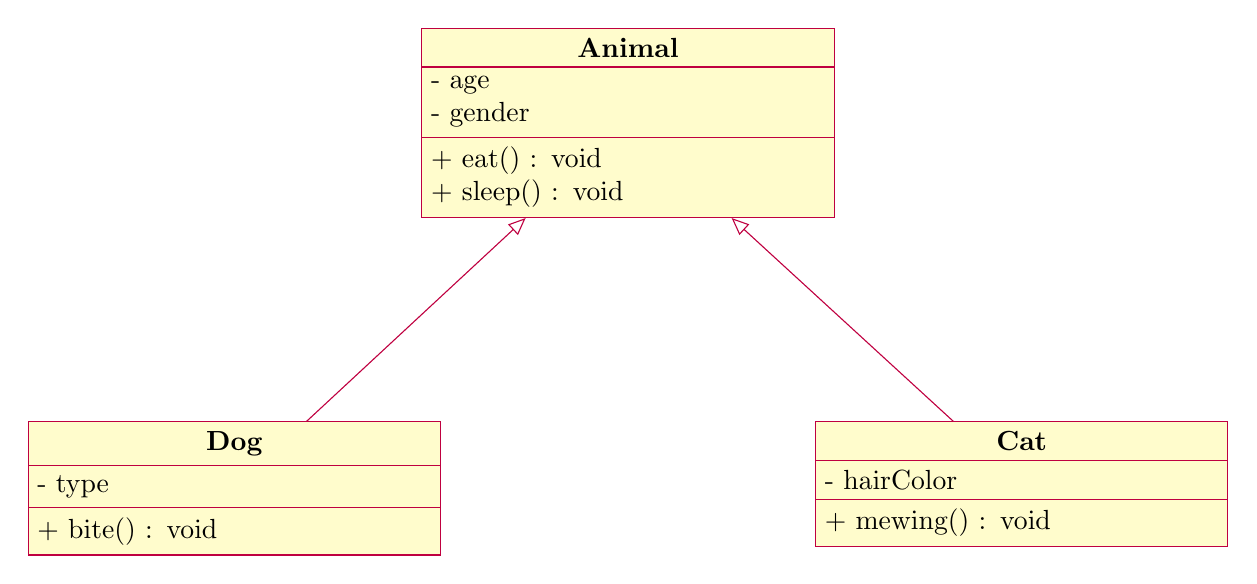
\begin{tikzpicture}
		\begin{class}{Animal}{0,0}
			\attribute{- age}
			\attribute{- gender}
			\operation{+ eat() : void}
			\operation{+ sleep() : void}
		\end{class}

		\begin{class}{Dog}{-5,-5}
			\inherit{Animal}
			\attribute{- type}
			\operation{+ bite() : void}
		\end{class}

		\begin{class}{Cat}{5,-5}
			\inherit{Animal}
			\attribute{- hairColor}
			\operation{+ mewing() : void}
		\end{class}
	\end{tikzpicture}
	\caption{继承}
\end{figure}

产生继承关系后,子类可以使用父类中的属性和方法,也可以定义子类独有的属性和方法。

\vspace{-0.5cm}

\begin{lstlisting}[language=C++]
class subclass : access_modifier superclass {
    // code
};
\end{lstlisting}

继承时通常使用public类型。当一个类public继承于父类时,父类的public成员也是子类的public成员,父类的protected成员也是子类的protected成员,父类的private成员不能被继承。\\

继承的好处是可以提高代码的复用性、提高代码的拓展性。\\

\mybox{继承}

\begin{lstlisting}[language=C++, title=animal.h]
#ifndef _ANIMAL_H_
#define _ANIMAL_H_

#include <string>

class Animal {
public:
    Animal(std::string name = "", int age = 0);
    void eat();

private:
    std::string name;
    int age;
};

#endif
\end{lstlisting}

\begin{lstlisting}[language=C++, title=animal.cpp]
#include "animal.h"
#include <iostream>

using namespace std;

Animal::Animal(string name, int age)
    : name(name), age(age) {}

void Animal::eat() {
    cout << "eating" << endl;
}
\end{lstlisting}

\begin{lstlisting}[language=C++, title=dog.h]
#ifndef _DOG_H
#define _DOG_H_

#include "animal.h"
#include <string>

class Dog : public Animal {
public:
    Dog(std::string name, int age, std::string type = "");
    void bite();
    
private:
    std::string type;
};

#endif
\end{lstlisting}

\begin{lstlisting}[language=C++, title=dog.cpp]
#include "dog.h"
#include <iostream>

using namespace std;

Dog::Dog(string name, int age, string type)
    : Animal(name, age), type(type) {}

void Dog::bite() {
    cout << "biting" << endl;
}
\end{lstlisting}

\begin{lstlisting}[language=C++, title=test\_dog.cpp]
#include <iostream>
#include "dog.h"

using namespace std;

int main() {
    Dog dog("狗子", 3, "哈士奇");
    dog.eat();
    dog.bite();
    return 0;
}
\end{lstlisting}

\begin{tcolorbox}
	\mybox{运行结果}
	\begin{verbatim}
eating
biting
	\end{verbatim}
\end{tcolorbox}

\newpage

\section{多继承}

\subsection{多继承}

C++支持多继承,即一个子类可以有两个或更多个父类。多继承时通过使用逗号将多个父类隔开,每个父类都可以用不同访问限定符修饰。\\

当多个父类中有同名的成员时,就会产生命名冲突,因此这时就需要在成员前加上类名和域限定符【::】消除二义性。\\

\mybox{多继承}

\begin{lstlisting}[language=C++, title=date.h]
#ifndef _DATE_H_
#define _DATE_H_

#include <string>

class Date {
public:
    Date(int year = 1970, int month = 1, int day = 1);
    std::string getDate();

private:
    int year;
    int month;
    int day;
};

#endif
\end{lstlisting}

\begin{lstlisting}[language=C++, title=date.cpp]
#include "date.h"

using namespace std;

Date::Date(int year, int month, int day)
    : year(year), month(month), day(day) {}

string Date::getDate() {
    char format[128];
    snprintf(format, sizeof(format), 
            "%04d/%02d/%02d", year, month, day);
    string dateStr(format);
    return dateStr;
}
\end{lstlisting}

\begin{lstlisting}[language=C++, title=time.h]
#ifndef _TIME_H_
#define _TIME_H_

#include <string>

class Time {
public:
    Time(int hour = 0, int minute = 0, int second = 0);
    std::string getTime();

private:
    int hour;
    int minute;
    int second;
};

#endif
\end{lstlisting}

\begin{lstlisting}[language=C++, title=time.cpp]
#include "time.h"

using namespace std;

Time::Time(int hour, int minute, int second)
    : hour(hour), minute(minute), second(second) {}

string Time::getTime() {
    char format[128];
    snprintf(format, sizeof(format), 
            "%02d:%02d:%02d", hour, minute, second);
    string timeStr(format);
    return timeStr;
}
\end{lstlisting}

\begin{lstlisting}[language=C++, title=date\_time.h]
#ifndef _DATE_TIME_H_
#define _DATE_TIME_H_

#include "date.h"
#include "time.h"
#include <string>

class DateTime : public Date, public Time {
public:
    DateTime(int year = 1970, int month = 1, int day = 1,
             int hour = 0, int minute = 0, int second = 0);
    std::string getDateTime();

private:
    int year;
    int month;
    int day;
    int hour;
    int minute;
    int second;
};

#endif
\end{lstlisting}

\begin{lstlisting}[language=C++, title=date\_time.cpp]
#include "date_time.h"

using namespace std;

DateTime::DateTime(int year, int month, int day,
         int hour, int minute, int second)
  : Date(year, month, day),
    Time(hour, minute, second) {}

string DateTime::getDateTime() {
    return getDate() + " " + getTime();
}
\end{lstlisting}

\begin{lstlisting}[language=C++, title=test\_date\_time.cpp]
#include <iostream>
#include "date_time.h"

using namespace std;

int main() {
    DateTime dt1;
    cout << dt1.getDateTime() << endl;
    DateTime dt2(2021, 8, 31, 13, 50, 23);
    cout << dt2.getDateTime() << endl;
    return 0;
}
\end{lstlisting}

\begin{tcolorbox}
	\mybox{运行结果}
	\begin{verbatim}
1970/01/01 00:00:00
2021/08/31 13:50:23
	\end{verbatim}
\end{tcolorbox}

\newpage

\section{向上转型与向下转型}

\subsection{向上转型 / 向下转型}

对象由子类类型转型为父类类型,即是向上转型。向上转型是一种隐式转换,一定会转型成功。向上转型后的对象,只能访问父类中定义的成员。\\

由父类类型转型转型为子类类型,即是向下转型。向下转型是不安全的,可能会导致数据的丢失,原因是父类的指针或引用中可能不包含子类成员的内存。\\

\mybox{向上转型}

\begin{lstlisting}[language=C++, title=animal.h]
#ifndef _ANIMAL_H_
#define _ANIMAL_H_

#include <string>

class Animal {
public:
    Animal(std::string name = "");
    std::string getName();

private:
    std::string name;
};

#endif
\end{lstlisting}

\begin{lstlisting}[language=C++, title=animal.cpp]
#include "animal.h"

using namespace std;

Animal::Animal(string name) : name(name) {}

string Animal::getName() {
    return name;
}
\end{lstlisting}

\begin{lstlisting}[language=C++, title=dog.h]
#ifndef _DOG_H_
#define _DOG_H_

#include "animal.h"
#include <string>

class Dog : public Animal {
public:
    Dog(std::string name, std::string type = "");
    std::string getType();

private:
    std::string type;
};

#endif
\end{lstlisting}

\begin{lstlisting}[language=C++, title=dog.cpp]
#include "dog.h"

using namespace std;

Dog::Dog(string name, string type) 
    : Animal(name), type(type) {}

string Dog::getType() {
    return type;
}
\end{lstlisting}

\begin{lstlisting}[language=C++, title=test\_dog.cpp]
#include <iostream>
#include "animal.h"
#include "dog.h"

using namespace std;

int main() {
    Dog dog("狗子", "哈士奇");
    cout << "dog: " << dog.getName()
         << ", " << dog.getType() << endl; 

    Animal animal = (Animal)dog;
    cout << "animal: " << animal.getName() << endl;
    return 0;
}
\end{lstlisting}

\begin{tcolorbox}
	\mybox{运行结果}
	\begin{verbatim}
dog: 狗子, 哈士奇
animal: 狗子
    \end{verbatim}
\end{tcolorbox}

\newpage
% \subsection{虚函数}

虚函数是定义在基类中的函数,子类必须对其进行重写/覆盖(override),虚函数需要在类的成员函数前面加上virtual关键字。\\

重写/覆盖是指子类中存在重新定义的函数,其函数名、参数列表、返回值类型都与父类中被重写的函数一致。被重写的函数必须是虚函数。\\

子类若重写了父类的函数,那么子类将会隐藏其父类中被重写的函数。但是子类通过强制类型转换成父类后可以重新调用父类中被重写的函数。\\

\subsection{纯虚函数}

在虚函数后加上【= 0】后可以让这个函数变成纯虚函数,包含纯虚函数的类叫做抽象类(abstract class)或接口类(interface)。\\

抽象类不能被用于实例化对象,只是提供了所有的子类共有的部分。例如在动物园中,存在的都是动物具体的子类对象,并不存在动物对象,所以动物类不应该被独立创建成对象。\\

抽象类的作用是可以被子类继承,提供共性的属性和方法。父类提供的方法很难满足子类不同的需求,如果不定义该方法,则表示所有的子类都不具有该行为。如果定义该方法,所有的子类都在重写,那么这个方法在父类中是没有必要实现的,显得多余。\\

被virtual关键字修饰的方法称为纯虚函数。纯虚函数只有声明,没有实现。纯虚函数只能包含在抽象类中。产生继承关系后,子类必须重写父类中所有的纯虚函数,否则子类还是抽象类。\\

\newpage
% \chapter{异常}

\section{异常}

\subsection{异常(Exception)}

异常就是程序在运行过程中出现的非正常的情况。异常本身是一个类,产生异常就是创建异常对象并抛出一个异常对象。Java处理异常的方法是中断处理。\\

C++异常处理涉及到三个关键字:

\begin{enumerate}
	\item throw:当问题出现时,程序会抛出一个异常。
	\item try:放置可能抛出异常的代码。
	\item catch:捕获并处理异常。
\end{enumerate}

\begin{figure}[H]
	\centering
	
\includegraphics{img/C15/15-1/1.png}
\end{figure}

\mybox{除以0}

\begin{lstlisting}[language=C++]
#include <iostream>

using namespace std;

int divide(int num1, int num2) {
    if(num2 == 0) {
        throw "division by zero";
    }
    return num1 / num2;
}

int main() {
    try {
        int result = divide(5, 0);
        cout << result << endl;
    } catch(const char *msg) {
        cerr << msg << endl;
    }

    return 0;
}
\end{lstlisting}

\begin{tcolorbox}
	\mybox{运行结果}
	\begin{verbatim}
division by zero
	\end{verbatim}
\end{tcolorbox}

普通的异常会导致程序无法完成编译,这样的异常被称为非运行时异常(non-runtime exception),但是由于异常是发生在编译时期的,因此常常称为编译时异常。在运行中如果遇到了异常,会导致程序执行的强制停止,这样的异常被称为运行时异常。

\newpage

\section{异常类}

C++提供了一系列标准的异常,定义在<exception>中。

\begin{table}[H]
	\centering
	\setlength{\tabcolsep}{5mm}{
		\begin{tabular}{|c|l|}
			\hline
			\textbf{异常}          & \textbf{描述}         \\
			\hline
			std::exception         & 所有标准C++异常的父类 \\
			\hline
			std::bad\_alloc        & 通过new抛出           \\
			\hline
			std::bad\_cast         & 通过dynamic\_cast抛出 \\
			\hline
			std::bad\_exception    & 处理无法预期的异常    \\
			\hline
			std::bad\_typeid       & 通过typeid抛出        \\
			\hline
			std::logic\_error      & 逻辑错误              \\
			\hline
			std::domain\_error     & 使用了无效的定义域    \\
			\hline
			std::invalid\_argument & 使用了无效的参数      \\
			\hline
			std::length\_error     & 创建过长的std::string \\
			\hline
			std::out\_of\_range    & 访问定义外的元素      \\
			\hline
			std::runtime\_error    & 运行时错误            \\
			\hline
			std::overflow\_error   & 发生上溢              \\
			\hline
			std::underflow\_error  & 发生下溢              \\
			\hline
			std::range\_error      & 存储超出范围的值      \\
			\hline
		\end{tabular}
	}
	\caption{异常类}
\end{table}

what()是异常类提供的一个公共方法,它已被所有子异常类重载。\\

\mybox{bad\_alloc}

\begin{lstlisting}[language=C++]
#include <iostream>
#include <exception>

using namespace std;

int main() {
    try {
        char *p = new char[0xfffffffff];
        delete p;
    } catch(bad_alloc &e) {
        cerr << e.what() << endl;
    }
    return 0;
}
\end{lstlisting}

\begin{tcolorbox}
	\mybox{运行结果}
	\begin{verbatim}
std::bad_alloc
	\end{verbatim}
\end{tcolorbox}

\newpage

\section{自定义异常}

\subsection{自定义异常}

系统中提供了很多的异常类型,但是异常类型提供地再多,也无法满足所有的需求。当需要的异常类型系统没有提供的时候,此时就需要自定义异常了。通过继承和重载exception类可以定义新的异常。\\

\mybox{自定义异常}

\begin{lstlisting}[language=C++]
#include <iostream>
#include <string>
#include <exception>

using namespace std;

class AgeException : public exception {
public:
    AgeException(string msg) : msg(msg) {}

    virtual const char* what() const noexcept override {
        return msg.c_str();
    }

private:
    string msg;
};

int main() {
    try {
        int age;
        cout << "Enter age: ";
        cin >> age;
        if(age < 0 || age > 130) {
            throw AgeException("invalid age");
        }
    } catch(AgeException& e) {
        cout << e.what() << endl;
    }

    return 0;
}
\end{lstlisting}

\begin{tcolorbox}
	\mybox{运行结果}
	\begin{verbatim}
Enter age: -1
invalid age
	\end{verbatim}
\end{tcolorbox}

\newpage
% \chapter{I/O库}

\section{文件I/O}

\subsection{文件I/O}

程序不仅要从控制台进行I/O,还需要读写文件和字符串。\\

标准库的I/O类型在3个头文件中:

\begin{enumerate}
	\item <iostream>定义了读写流的基本类型。
	\item <fstream>定义了读写文件的类型。
	\item <sstream>定义了读写string对象的类型。
\end{enumerate}

<fstream>中定义了3个I/O类来读写文件:

\begin{enumerate}
	\item ifstream从给定文件读数据。
	\item ofstream向给定文件写数据。
	\item fstream可读写文件。
\end{enumerate}

\vspace{0.5cm}

\subsection{文件打开模式}

每个流都有一个关联的文件模式,在打开文件时可以指定文件模式。

\begin{table}[H]
	\centering
	\setlength{\tabcolsep}{5mm}{
		\begin{tabular}{|c|l|}
			\hline
			\textbf{打开模式} & \textbf{作用}                                   \\
			\hline
			ios::in           & 以读方式打开                                    \\
			\hline
			ios::out          & 以写方式打开                                    \\
			\hline
			ios::app          & 以追加方式打开                                  \\
			\hline
			ios::ate          & 打开文件定位到文件末尾                          \\
			\hline
			ios::trunc        & 如果文件存在,其内容将被截断,即把文件长度设为0 \\
			\hline
		\end{tabular}
	}
	\caption{文件打开模式}
\end{table}

\mybox{文件I/O}

\begin{lstlisting}[language=C++]
#include <iostream>
#include <fstream>

using namespace std;

int main() {
    string name;
    int id;
    cout << "Enter name: ";
    cin >> name;
    cout << "Enter id: ";
    cin >> id;
    
    ofstream out("info.txt");
    out << name << " " << id << endl;
    out.close();
    
    ifstream in("info.txt");
    in >> name >> id;
    in.close();
    
    cout << "name = " << name << ", id = " << id << endl;
    return 0;
}
\end{lstlisting}

\begin{tcolorbox}
	\mybox{运行结果}
	\begin{verbatim}
Enter name: Terry
Enter id: 979489
name = Terry, id = 979489
	\end{verbatim}
\end{tcolorbox}

\newpage
% \chapter{STL标准模板库}

\section{模板}

\subsection{泛型编程(Generic Programming)}

面向对象编程(OOP)和泛型编程(GP)都能处理在编写程序时类型未知的情况,OOP能处理运行时获取类型的情况,GP能处理编译期可获取类型的情况。\\

模板是泛型编程的基础,泛型编程就是以一种独立于任何特定类型的方式编写代码。C++标准库的容器、迭代器、算法都是泛型编程的例子。\\

\subsection{函数模板}

通过定义一个通用的函数模板可以处理参数为多种类型的情形,而不是为每个类型都定义一个重载。模板定义使用template关键字,后跟模板参数列表。模板参数表示函数或类定义中用到的类型,使用模板时需要隐式或显式提供模板实参,将其绑定到模板参数。\\

\mybox{函数模板}

\begin{lstlisting}[language=C++]
#include <iostream>
#include <string>

using namespace std;

template <typename T>
inline T getMax(const T& val1, const T& val2) {
    return val1 > val2 ? val1 : val2;
}

int main() {
    int iVal1 = 28;
    int iVal2 = 92;
    cout << getMax(iVal1, iVal2) << endl;

    double dVal1 = 3.14;
    double dVal2 = 3.71;
    cout << getMax(dVal1, dVal2) << endl;

    string sVal1 = "hello";
    string sVal2 = "world";
    cout << getMax(sVal1, sVal2) << endl;
    return 0;
}
\end{lstlisting}

\begin{tcolorbox}
	\mybox{运行结果}
	\begin{verbatim}
92
3.71
world
	\end{verbatim}
\end{tcolorbox}

函数模板仅仅是函数的规范,本身并不会占用内存。当编译器遇到对模板函数的调用时,才会在内存中创建该函数的实例。\\

\subsection{类模板}

类模板用来生成类的蓝图,与函数模板不同的是,类模板在实例化时编译器无法为类模板推导模板参数类型,而是必须在模板名后用【<>】提供实参。根据显式提供的模板实参列表,编译器使用这些模板参数来实例化特定的类。\\

编译器从类模板实例化一个类时,会重写模板,将模板参数的每个实例替换为给定的模板实参。因此类模板的每个实例都是独立的类,使用不同模板实参实例化出的类之间没有关联,也没有特殊的访问权限。\\

\mybox{类模板}

\begin{lstlisting}[language=C++]
#include <iostream>
#include <sstream>
#include <algorithm>

using namespace std;

template<class T>
class SortedArray {
public:
    SortedArray(int capacity = 1);
    SortedArray(T *arr, int capacity);
    ~SortedArray();

    string data();
    void add(T val);
    void remove(T val);

private:
    T *arr;
    int len;
    int capacity;
    void resize(int size);
};

template<class T>
SortedArray<T>::SortedArray(int capacity) {
    this->len = 0;
    this->capacity = capacity;
    this->arr = new T[capacity];
}

template<class T>
SortedArray<T>::SortedArray(T *arr, int len) {
    this->len = len;
    this->capacity = len;
    this->arr = new T[len];
    for(int i = 0; i < len; i++) {
        this->arr[i] = arr[i];
    }
}

template<class T>
SortedArray<T>::~SortedArray() {
    delete arr;
}

template<class T>
string SortedArray<T>::data() {
    if(len == 0) {
        return "[]";
    }

    sort(this->arr, this->arr + len);
    ostringstream out;
    out << "[";
    for(int i = 0; i < len; i++) {
        out << arr[i] << ", ";
    }
    out << "\b\b]";
    return out.str();
}

template<class T>
void SortedArray<T>::resize(int size) {
    T *temp = new T[size];
    for(int i = 0; i < len; i++) {
        temp[i] = arr[i];
    }
    delete arr;
    arr = temp;
}

template<class T>
void SortedArray<T>::add(T val) {
    if(len == capacity) {
        capacity *= 2;
        resize(capacity);
    }
    arr[len++] = val;
}

template<class T>
void SortedArray<T>::remove(T val) {
    for(int i = 0; i < len; i++) {
        if(arr[i] == val) {
            arr[i] = arr[len-1];
            len--;
            if(len <= capacity / 2) {
                capacity /= 2;
                resize(capacity);
            }
            break;
        }
    }
}

int main() {
    int arr[] = {7, 7, 3, 9, 7, 1, 3};
    int n = sizeof(arr) / sizeof(arr[0]);

    SortedArray<int> sortedArray(arr, n);
    cout << sortedArray.data() << endl;

    sortedArray.add(28);
    sortedArray.add(12);
    cout << sortedArray.data() << endl;

    sortedArray.remove(7);
    sortedArray.remove(9);
    cout << sortedArray.data() << endl;

    return 0;
}
\end{lstlisting}

\begin{tcolorbox}
	\mybox{运行结果}
	\begin{verbatim}
[1, 3, 3, 7, 7, 7, 9] 
[1, 3, 3, 7, 7, 7, 9, 12, 28]
[1, 3, 3, 7, 7, 12, 28]
	\end{verbatim}
\end{tcolorbox}

\newpage

\section{容器}

\subsection{容器(Container)}

容器是特定类型对象的集合,容器分为顺序容器和关联容器:

\begin{itemize}
	\item 顺序容器:元素的顺序与其加入容器的位置对应。
	\item 关联容器:元素的顺序由其关联的关键字决定,关联容器分为有序关联容器和无序关联容器。
\end{itemize}

所有容器类共享公有接口,不同容器按不同方式扩展。\\

C++新标准容器的性能比旧版本快很多,其性能与最精心优化过的同类数据结构一样好。现代C++程序应该使用标准库容器,而不是更原始的数据结构。\\

\subsection{顺序容器}

每个容器都定义于一个头文件中,文件名与容器名相同。容器都定义为模板类,顺序容器几乎可以保存任意类型的元素,还可以在容器中保存容器。

\begin{table}[H]
	\centering
	\setlength{\tabcolsep}{5mm}{
		\begin{tabular}{|c|l|}
			\hline
			\textbf{容器} & \textbf{描述}                                      \\
			\hline
			array         & 固定大小数组,支持快速随机访问,不能增删元素       \\
			\hline
			vector        & 可变大小数组,支持快速随机访问,非尾部位置增删较慢 \\
			\hline
			string        & 专门用于保存字符,随机访问快,在尾部增删速度快     \\
			\hline
			deque         & 双端队列,支持快速随机访问,在头尾位置增删速度很快 \\
			\hline
			list          & 双向链表,支持双向顺序访问,在任何位置增删都很快   \\
			\hline
			forward\_list & 单向链表,只支持单向顺序访问,在任何位置增删都很快 \\
			\hline
		\end{tabular}
	}
	\caption{顺序容器}
\end{table}

array和内置数组一样大小固定,但操作更安全。除固定大小的array外,其它容器都提供高效灵活的内存管理,可以添加、删除、扩展和收缩容器的大小。\\

vector和string将元素存储在连续空间中,故通过下标的随机访问很快。在尾部添加元素很快,但中间和头部插入或删除很慢。添加元素可能造成空间的重新分配和元素拷贝。\\

deque支持快速随机访问,在两端插入或删除很快,但在中间插入或删除元素很慢。\\

list和forward\_list的设计目的是让任何位置的插入或删除都快速高效且不需重新分配内存,但是不支持随机访问,为访问一个元素需要遍历整个链表。\\

\subsection{迭代器(Iterator)}

迭代器比下标访问更通用,所有标准库容器都支持迭代器,但只有几种支持下标。迭代器提供了对容器对象的间接访问,类似于指针。begin()返回指向首元素的迭代器,end()返回指向尾元素下一位置(尾后)的迭代器。如果容器为空,则begin()和end()返回的都是尾后迭代器。任何可能改变容器容量的操作都会使容器的迭代器失效。

\begin{table}[H]
	\centering
	\setlength{\tabcolsep}{5mm}{
		\begin{tabular}{|l|l|}
			\hline
			\textbf{容器}            & \textbf{描述}                  \\
			\hline
			iterator                 & 容器的迭代器                   \\
			\hline
			begin()                  & 返回指向首元素的迭代器         \\
			\hline
			end()                    & 返回尾后迭代器                 \\
			\hline
			const\_iterator          & 只读迭代器                     \\
			\hline
			cbegin()                 & 返回指向首元素的只读迭代器     \\
			\hline
			cend()                   & 返回尾后只读迭代器             \\
			\hline
			reverse\_iterator        & 按逆序寻址元素的迭代器         \\
			\hline
			rbegin()                 & 返回指向尾元素的逆序迭代器     \\
			\hline
			rend()                   & 返回首前逆序迭代器             \\
			\hline
			const\_reverse\_iterator & 只读逆序迭代器                 \\
			\hline
			crbegin()                & 返回指向尾元素的只读逆序迭代器 \\
			\hline
			crend()                  & 返回首前只读逆序迭代器         \\
			\hline
		\end{tabular}
	}
	\caption{迭代器}
\end{table}

迭代器可以进行算术运算,将迭代器与整数相加减可以得到向前或向后若干位置的迭代器。使用关系运算符【<】、【<=】、【>】、【>=】和【==】可以对迭代器所指位置比较大小。将两个迭代器相减,结果是两个迭代器的距离。\\

\mybox{迭代器}

\begin{lstlisting}[language=C++]
#include <iostream>
#include <string>

using namespace std;

int main() {
    string s = "hello world";

    string::iterator iter = s.begin();
    cout << "[";
    while(iter != s.end()) {
        cout << *iter << ", ";
        iter++;
    }
    cout << "\b\b]" << endl;

    return 0;
}
\end{lstlisting}

\begin{tcolorbox}
	\mybox{运行结果}
	\begin{verbatim}
[h, e, l, l, o,  , w, o, r, l, d]
	\end{verbatim}
\end{tcolorbox}

\newpage

\section{STL数组}

\subsection{array}

array容器是C++11标准中新增的序列容器,它在普通数组的基础上,添加了一些成员函数和全局函数。在使用上,它比普通数组更安全,且效率并没有因此变差。和其它容器不同,array的大小是固定的,无法动态的扩展或收缩。与内置数组不同的是,array允许做整个容器的拷贝和赋值,要求两个array大小和元素类型都一样。\\

array以类模板的形式定义在<array>头文件,array具有固定大小,其大小也是类型的一部分,定义时模板参数包含元素类型和大小。

\begin{table}[H]
	\centering
	\setlength{\tabcolsep}{5mm}{
		\begin{tabular}{|c|l|}
			\hline
			\textbf{成员函数} & \textbf{功能}                            \\
			\hline
			size()            & 返回容器中当前元素的数量                 \\
			\hline
			max\_size()       & 返回容器可容纳元素的最大数量             \\
			\hline
			empty()           & 判断容器是否为空                         \\
			\hline
			at(n)             & 返回容器中第n个元素的引用                \\
			\hline
			front()           & 返回容器中第一个元素的直接引用           \\
			\hline
			back()            & 返回容器中最后一个元素的直接应用         \\
			\hline
			data()            & 返回一个指向容器首个元素的指针           \\
			\hline
			fill(val)         & 将val赋值给容器中的每个元素              \\
			\hline
			arr1.swap(arr2)   & 交换相同长度和类型的arr1和arr2中所有元素 \\
			\hline
		\end{tabular}
	}
	\caption{array成员函数}
\end{table}

\mybox{array}

\begin{lstlisting}[language=C++]
#include <iostream>
#include <array>

using namespace std;

int main() {
    array<int, 10> arr = {0, 1, 2, 3, 4, 5, 6, 7, 8, 9};
    cout << "size = " << arr.size() << endl;
    array<int, 10>::iterator begin = arr.begin();
    array<int, 10>::iterator end = arr.end();
    while(begin != end) {
        cout << *begin << " ";
        begin++;
    }
    cout << endl;
    return 0;
}
\end{lstlisting}

\begin{tcolorbox}
	\mybox{运行结果}
	\begin{verbatim}
size = 10
0 1 2 3 4 5 6 7 8 9
	\end{verbatim}
\end{tcolorbox}

\vspace{0.5cm}

\subsection{vector}

vector表示对象的集合,由于vector容纳其它的对象,所以是一种容器。使用vector需要包含头文件<vector>。vector是一个类模板,模板可以看作编译器生成类或函数的一份说明。

\begin{table}[H]
	\centering
	\setlength{\tabcolsep}{5mm}{
		\begin{tabular}{|l|l|}
			\hline
			\textbf{初始化}              & \textbf{功能}                            \\
			\hline
			vector<T> v                  & 创建一个空的vector                       \\
			\hline
			vector<T> v2(v1)             & 用v1中所有元素的副本创建v2               \\
			\hline
			vector<T> v2 = v1            & 等价于v2(v1)                             \\
			\hline
			vector<T> v(n, val)          & v中包含了n个值为val的元素                \\
			\hline
			vector<T> v(n)               & v中包含了n个值为默认初始化的元素         \\
			\hline
			vector<T> v{a, b, c, ...}    & 用列表元素初始化v                        \\
			\hline
			vector<T> v = {a, b, c, ...} & 等价于v{a, b, c, ...}                    \\
			\hline
			vector<T> v (begin, end)     & 根据迭代器范围[begin, end)复制到vector中 \\
			\hline
		\end{tabular}
	}
	\caption{vecor初始化}
\end{table}

\mybox{vector初始化}

\begin{lstlisting}[language=C++]
#include <iostream>
#include <string>
#include <vector>
#include <algorithm>
#include <iterator>

using namespace std;

template <typename T>
ostream& operator<<(ostream& out, const vector<T>& v) {
    if(!v.empty()) {
        out << "[";
        copy(v.begin(), v.end(), ostream_iterator<T>(out, ", "));
        out << "\b\b]";
    }
    return out;
}

int main() {
    vector<int> v1(10);         // 有10个元素,都是0
    vector<int> v2{10};         // 有1个元素,值是10
    vector<int> v3(10, 1);      // 有10个元素,都是1
    vector<int> v4{10, 1};      // 有2个元素,10和1
    vector<string> v5{"hello"}; // 有1个元素,是字符串"hello"
    
    cout << "v1 = " << v1 << endl;
    cout << "v2 = " << v2 << endl;
    cout << "v3 = " << v3 << endl;
    cout << "v4 = " << v4 << endl;
    cout << "v5 = " << v5 << endl;
    return 0;
}
\end{lstlisting}

\begin{tcolorbox}
	\mybox{运行结果}
	\begin{verbatim}
v1 = [0, 0, 0, 0, 0, 0, 0, 0, 0, 0] 
v2 = [10] 
v3 = [1, 1, 1, 1, 1, 1, 1, 1, 1, 1] 
v4 = [10, 1]
v5 = [hello]
	\end{verbatim}
\end{tcolorbox}

\vspace{0.5cm}

\subsection{vector操作}

\begin{table}[H]
	\centering
	\setlength{\tabcolsep}{5mm}{
		\begin{tabular}{|l|l|}
			\hline
			\textbf{操作}       & \textbf{功能}                              \\
			\hline
			v.empty()           & 判断vector是否为空                         \\
			\hline
			v.size()            & 返回vector元素个数                         \\
			\hline
			v[n]                & 返回vector中第n个元素的引用                \\
			\hline
			v1 = v2             & 用v2中的元素拷贝替换v1中的元素             \\
			\hline
			v1 == v2、v1 != v2  & v1和v2相等当且仅当元素个数和对应元素都相同 \\
			\hline
			v.push\_back(val)   & 向vector尾部添加一个元素                   \\
			\hline
			v.insert(iter, val) & 向迭代器指向元素前添加一个元素             \\
			\hline
			v.pop\_back()       & 删除vector最后一个元素                     \\
			\hline
			v.erase(iter)       & 删除迭代器指向元素                         \\
			\hline
			v.erase(begin, end) & 删除迭代器返回[begin, end)范围元素         \\
			\hline
			v.clear()           & 清空vector                                 \\
			\hline
			v.swap(vector)      & 交换两个同类型vector数据                   \\
			\hline
			v.assign(n, val)    & 设置vector中前n个元素值为val               \\
			\hline
		\end{tabular}
	}
	\caption{vector操作}
\end{table}

vector不能使用下标添加元素,否则会造成缓冲区溢出,确保下标合法的一种有效手段就是尽可能使用for-each循环。如果循环体内部包含向vector添加元素的语句,则不能使用for-each循环。\\

\mybox{vector}

\begin{lstlisting}[language=C++]
#include <iostream>
#include <vector>

using namespace std;

int main() {
    vector<int> v;
    for(int i = 0; i < 10; i++) {
        v.push_back(i * i);
    }

    for(int& item : v) {
        cout << item << " ";
    }
    cout << endl;
    return 0;
}
\end{lstlisting}

\begin{tcolorbox}
	\mybox{运行结果}
	\begin{verbatim}
0 1 4 9 16 25 36 49 64 81
	\end{verbatim}
\end{tcolorbox}

\newpage

\section{STL字符串}

\subsection{string}

string是标准库中的类型,表示可变长字符序列,使用需要包含头文件<string>。\\

string的初始化分为:

\begin{enumerate}
	\item 直接初始化:使用括号初始化,调用构造函数。
	\item 拷贝初始化:使用赋值初始化,调用重载的赋值运算符。
\end{enumerate}

\vspace{0.5cm}

\mybox{string初始化}

\begin{lstlisting}[language=C++]
#include <iostream>
#include <string>

using namespace std;

int main() {
    string s1;              // 默认初始化,为空字符串
    string s2(s1);          // 直接初始化,s2是s1的副本
    string s3 = s1;         // 拷贝初始化,s3是s1的副本,等价s3(s1)
    string s4("hello");     // 直接初始化,初始化为字面值常量
    string s5 = "hello";    // 拷贝初始化,初始化为字面值常量
    string s6(10, 'x');     // 直接初始化,初始化为10个字符'x'
    
    cout << "s1 = " << s1 << endl;
    cout << "s2 = " << s2 << endl;
    cout << "s3 = " << s3 << endl;
    cout << "s4 = " << s4 << endl;
    cout << "s5 = " << s4 << endl;
    cout << "s6 = " << s4 << endl;
    
    return 0;
}
\end{lstlisting}

\begin{tcolorbox}
	\mybox{运行结果}
	\begin{verbatim}
s1 = 
s2 =
s3 =
s4 = hello
s5 = hello
s6 = hello
	\end{verbatim}
\end{tcolorbox}

\vspace{0.5cm}

\subsection{string操作}

\begin{table}[H]
	\centering
	\setlength{\tabcolsep}{5mm}{
		\begin{tabular}{|l|l|}
			\hline
			\textbf{操作}          & \textbf{功能}                                 \\
			\hline
			out << s               & 将s写到输出流out中                            \\
			\hline
			in >> s                & 从输入流中读取字符串赋给s,字符串以空白符分割 \\
			\hline
			getline(in, s)         & 从输入流中读取一行赋给s                       \\
			\hline
			s.empty()              & 判断s是否为空                                 \\
			\hline
			s.size()               & 返回s中字符个数                               \\
			\hline
			s[n]                   & 返回s中第n个字符的引用                        \\
			\hline
			s1 + s2                & 返回s1和s2连接后的结果                        \\
			\hline
			s1 = s2                & 用s2的副本替换s1                              \\
			\hline
			s1 == s2、s1 != s2     & 判断s1和s2是否相等                            \\
			\hline
			<、<=、>、>=           & 字典序比较,对大小写敏感                      \\
			\hline
			s1.append(s2)          & 尾部插入                                      \\
			\hline
			s1.insert(pos, s2)     & 在第pos个位置插入s2                           \\
			\hline
			s.erase(pos, n)        & 从第pos个位置删除n个字符                      \\
			\hline
			s1.replace(pos, n, s2) & 从第pos个位置开始替换n个字符为s2              \\
			\hline
			s.substr(pos, n)       & 返回一个从pos开始的n个字符的拷贝              \\
			\hline
			s1.find(s2)            & 查找s1中s2第一次出现的位置                    \\
			\hline
			s1.rfind(s2)           & 查找s1中s2最后一次出现的位置                  \\
			\hline
		\end{tabular}
	}
	\caption{string操作}
\end{table}

\mybox{string}

\begin{lstlisting}[language=C++]
#include <iostream>
#include <string>

using namespace std;

int main() {
    string s("Hello");

    s.append("world");          // Helloworld
    s.insert(s.size(), "!");    // Helloworld!

    s.replace(1, 4, "i");       // Hiworld!
    s.erase(2, 5);              // Hi!
    s.insert(2, " C++");        // Hi C++!

    cout << s << endl;

    cout << s.substr(3, 3) << endl;
    cout << s.substr(3) << endl;
    cout << s.find("C++") << endl;

    return 0;
}
\end{lstlisting}

\begin{tcolorbox}
	\mybox{运行结果}
	\begin{verbatim}
Hi C++!
C++
C++!
3
	\end{verbatim}
\end{tcolorbox}

\newpage

\section{STL链表}

\subsection{list}

list双向链表通过指针连成逻辑意义上的线性表,由于list中结点并不要求在一段连续内存中,因此list不支持快速随机存取,迭代器只能通过【++】或【--】移动。\\

\begin{figure}[H]
	\centering
	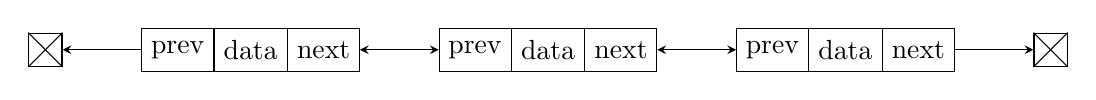
\begin{tikzpicture}[list/.style={rectangle split, rectangle split parts=3,
					draw, rectangle split horizontal}, >=stealth, start chain]
		\node[on chain,draw,inner sep=6pt] (NULL1) {};
		\node[list,on chain] (A) {prev \nodepart{second} data \nodepart{third} next};
		\node[list,on chain] (B) {prev \nodepart{second} data \nodepart{third} next};
		\node[list,on chain] (C) {prev \nodepart{second} data \nodepart{third} next};
		\node[on chain,draw,inner sep=6pt] (NULL2) {};
		\draw (NULL1.north east) -- (NULL1.south west);
		\draw (NULL1.north west) -- (NULL1.south east);
		\draw (NULL2.north east) -- (NULL2.south west);
		\draw (NULL2.north west) -- (NULL2.south east);
		\draw[<-] let \p1 = (A.west), \p2 = (A.center) in (NULL1) -- (\x1,\y2);
		\draw[<->] let \p1 = (A.east), \p2 = (A.center) in (\x1,\y2) -- (B);
		\draw[<->] let \p1 = (B.east), \p2 = (B.center) in (\x1,\y2) -- (C);
		\draw[->] let \p1 = (C.east), \p2 = (C.center) in (\x1,\y2) -- (NULL2);
	\end{tikzpicture}
	\caption{双向链表}
\end{figure}

\begin{table}[H]
	\centering
	\setlength{\tabcolsep}{5mm}{
		\begin{tabular}{|l|l|}
			\hline
			\textbf{操作}      & \textbf{功能}         \\
			\hline
			list<T> lst        & 创建空的list          \\
			\hline
			list<T> lst(n)     & 创建含有n个元素的list \\
			\hline
			list<T> lst1(lst2) & 使用lst2初始化lst1    \\
			\hline
			lst.size()         & 返回list元素个数      \\
			\hline
			lst.clear()        & 删除所有元素          \\
			\hline
			lst.empty()        & 判断list是否为空      \\
			\hline
			lst.front()        & 返回第一个元素        \\
			\hline
			lst.back()         & 返回最后一个元素      \\
			\hline
			lst.insert()       & 插入一个元素          \\
			\hline
			lst.erase()        & 删除一个元素          \\
			\hline
			lst.push\_front()  & 在头部添加一个元素    \\
			\hline
			lst.push\_back()   & 在尾部添加一个元素    \\
			\hline
			lst.pop\_front()   & 删除第一个元素        \\
			\hline
			lst.pop\_back()    & 删除最后一个元素      \\
			\hline
			lst.remove()       & 删除元素              \\
			\hline
			lst.reverse()      & 反转list              \\
			\hline
			lst.sort()         & 排序                  \\
			\hline
			lst.unique()       & 去除相邻的重复元素    \\
			\hline
			lst.merge()        & 合并两个有序list      \\
			\hline
		\end{tabular}
	}
	\caption{list操作}
\end{table}

其中,lst.unique()并不是把重复的元素删除,而是全部放到数组尾部,返回去重后的尾地址。unique()中不自带sort(),因此需要先使用sort()进行排序。\\

\mybox{list}

\begin{lstlisting}[language=C++]
#include <iostream>
#include <list>

using namespace std;

void printList(list<int> lst) {
    for(list<int>::iterator iter = lst.begin();
                            iter != lst.end();
                            iter++) {
        cout << *iter << " ";
    }
    cout << endl;
}

int main() {
    list<int> lst;

    lst.push_back(11);       // [11]
    lst.push_front(22);      // [22, 11]
    cout << lst.front() << endl;    // 22
    cout << lst.back() << endl;     // 11

    lst.insert(++lst.begin(), 3);   // [22, 3, 11]
    lst.insert(--lst.end(), 2);     // [22, 3, 2, 11]
    lst.push_back(2);               // [22, 3, 2, 11, 2]
    printList(lst);

    lst.pop_front();                // [3, 2, 11, 2]
    lst.sort();                     // [2, 2, 3, 11]
    lst.unique();                   // [2, 3, 11]
    printList(lst);

    lst.sort();                     // [2, 3, 11]
    printList(lst);

    list<int> lst2{1, 2, 8};
    lst.merge(lst2);                // [1, 2, 2, 3, 8, 11]
    printList(lst);

    return 0;
}
\end{lstlisting}

\begin{tcolorbox}
	\mybox{运行结果}
	\begin{verbatim}
22
11
22 3 2 11 2
2 3 11
2 3 11
1 2 2 3 8 11
	\end{verbatim}
\end{tcolorbox}

\vspace{0.5cm}

\subsection{forward\_list}

forward\_list和list的区别在于前者是单向链表,每个元素内部只有一个链接指向下一个元素,因此在存储方面list会消耗更多的空间。\\

\begin{figure}[H]
	\centering
	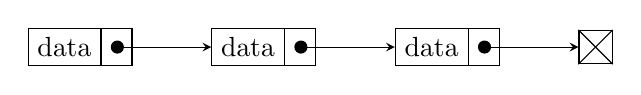
\begin{tikzpicture}[list/.style={rectangle split, rectangle split parts=2,
					draw, rectangle split horizontal}, >=stealth, start chain]
		\node[list,on chain] (A) {data};
		\node[list,on chain] (B) {data};
		\node[list,on chain] (C) {data};
		\node[on chain,draw,inner sep=6pt] (D) {};
		\draw (D.north east) -- (D.south west);
		\draw (D.north west) -- (D.south east);
		\draw[*->] let \p1 = (A.two), \p2 = (A.center) in (\x1,\y2) -- (B);
		\draw[*->] let \p1 = (B.two), \p2 = (B.center) in (\x1,\y2) -- (C);
		\draw[*->] let \p1 = (C.two), \p2 = (C.center) in (\x1,\y2) -- (D);
	\end{tikzpicture}
	\caption{单向链表}
\end{figure}

forward\_list不支持反向迭代器,并且没有指向尾元素的迭代器,因此不提供back()、push\_back()、pop\_back()等操作。

\newpage

\section{容器适配器}

\subsection{stack}

栈,又名堆栈,是一种运算受限的线性数据结构,栈只能在表尾进行插入和删除操作。\\

栈中的元素只能先进后出(FILO, First In Last Out)。最早进入栈的元素所存放的位置叫作栈底(bottom),最后进入栈的元素存放的位置叫作栈顶(top)。\\

\begin{figure}[H]
	\centering
	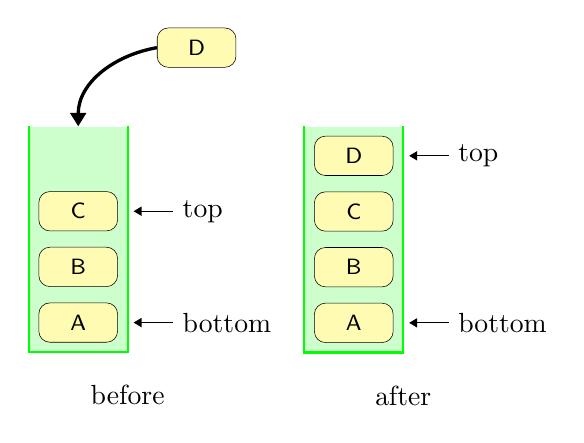
\begin{tikzpicture}
		\matrix[queue] (Q1) {
		|[fill=none, draw=none]|\\
		|(front)| C\\
		B\\
		|(rear)| A\\};
		\draw[green,thick,-] (Q1.north west) |-(Q1.south)-| (Q1.north east);
		\draw[<-] ([xshift=.2cm]front.east) -- ++ (0:.5) node[right] {top};
		\draw[<-] ([xshift=.2cm]rear.east) -- ++ (0:.5) node[right] {bottom};
		\draw[<-,very thick] (Q1.north) to[out=90,in=190] ++ (1,1) node[right, queue element] (D) {D};
		\node[below=3mm of Q1.south east] {before};

		\scope[xshift=3.5cm]
		\matrix[queue] (Q1) {
			|(front)| D \\
			C           \\
			B           \\
			|(rear)| A\\};
		\draw[green,thick,-] (Q1.north west) |-(Q1.south)-| (Q1.north east);
		\draw[<-] ([xshift=.2cm]front.east) -- ++ (0:.5) node[right] {top};
		\draw[<-] ([xshift=.2cm]rear.east) -- ++ (0:.5) node[right] {bottom};
		\node[below=3mm of Q1.south east] {after};
		\endscope
	\end{tikzpicture}
	\caption{栈}
\end{figure}

向一个栈插入新元素的操作称为入栈push(或进栈、压栈),从一个栈删除元素的操作称为出栈pop(或退栈、弹栈)。入栈操作就是把新元素放入栈中,只允许从栈顶一侧放入元素,新元素的位置将会成为新的栈顶。出栈操作就是把新元素从栈中弹出,只有栈顶元素才允许出栈,出栈元素的前一个元素将会成为新的栈顶。

\begin{table}[H]
	\centering
	\setlength{\tabcolsep}{5mm}{
		\begin{tabular}{|l|l|}
			\hline
			\textbf{操作} & \textbf{功能}                        \\
			\hline
			empty()       & 判断栈是否为空                       \\
			\hline
			size()        & 返回栈中元素个数                     \\
			\hline
			push()        & 入栈,调用底层容器的push\_back()实现 \\
			\hline
			pop()         & 出栈                                 \\
			\hline
			top()         & 返回栈顶元素的引用                   \\
			\hline
		\end{tabular}
	}
	\caption{stack操作}
\end{table}

\mybox{stack}

\begin{lstlisting}[language=C++]
#include <iostream>
#include <stack>

using namespace std;

int main() {
	stack<int> s;
	s.push(1);
	s.push(2);
	s.push(3);
	cout << s.top() << endl;

	while(!s.empty()) {
		cout << s.top() << endl;
		s.pop();
	}
	return 0;
}
\end{lstlisting}

\begin{tcolorbox}
	\mybox{运行结果}
	\begin{verbatim}
3
3
2
1
	\end{verbatim}
\end{tcolorbox}

\vspace{0.5cm}

\subsection{deque}

deque双端队列是一种同时具有队列和栈的性质的数据结构,双端队列可以从其两端插入和删除元素。

\begin{figure}[H]
	\centering
	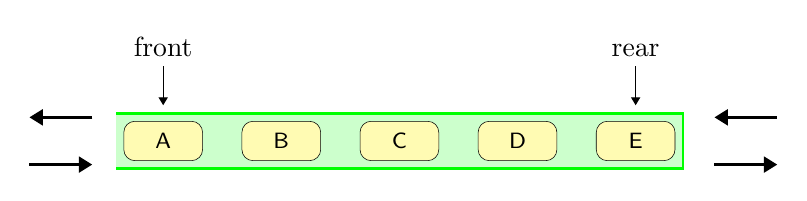
\begin{tikzpicture}
		\fill[green!20] (6.6,.35) rectangle (-.6,-.35);
		\draw[green,thick] (-.6,.35) -- (6.6,.35) |- (-.6,-.35);
		\foreach \i/\name in {0/A,1/B,2/C,3/D,4/E}
		\node[queue element] (\name) at (1.5*\i,0) {\name};
		\draw[<-] ([yshift=.2cm]E.north) -- ++ (0,.5) node[above] {rear};
		\draw[<-] ([yshift=.2cm]A.north) -- ++ (0,.5) node[above] {front};

		\draw[->,very thick] (-0.9,0.3) -- (-1.7,0.3);
		\draw[->,very thick] (-1.7,-0.3) --  (-0.9,-0.3);

		\draw[<-,very thick] (7,0.3) -- (7.8,0.3);
		\draw[<-,very thick] (7.8,-0.3) -- (7,-0.3);
	\end{tikzpicture}
	\caption{双端队列}
\end{figure}

\begin{table}[H]
	\centering
	\setlength{\tabcolsep}{5mm}{
		\begin{tabular}{|l|l|}
			\hline
			\textbf{操作} & \textbf{功能}       \\
			\hline
			empty()       & 判断deque是否为空   \\
			\hline
			size()        & 返回deque中元素个数 \\
			\hline
			front()       & 返回首元素引用      \\
			\hline
			back()        & 返回尾元素引用      \\
			\hline
			push\_front() & 在头部添加一个元素  \\
			\hline
			push\_back()  & 在尾部添加一个元素  \\
			\hline
			pop\_front()  & 在头部删除一个元素  \\
			\hline
			pop\_back()   & 在尾部删除一个元素  \\
			\hline
			clear()       & 清空deque           \\
			\hline
		\end{tabular}
	}
	\caption{deque操作}
\end{table}

\mybox{deque}

\begin{lstlisting}[language=C++]
#include <iostream>
#include <deque>

using namespace std;

int main() {
	deque<int> deq;
	
	deq.push_front(1);
	deq.push_front(2);
	deq.push_back(3);
	deq.push_back(4);
	cout << deq.front() << endl;
	cout << deq.back() << endl;

	deq.pop_back();
	deq.pop_front();
	cout << deq.front() << endl;
	cout << deq.back() << endl;

	return 0;
}
\end{lstlisting}

\begin{tcolorbox}
	\mybox{运行结果}
	\begin{verbatim}
2
4
1
3
	\end{verbatim}
\end{tcolorbox}

\vspace{0.5cm}

\subsection{priority\_queue}

普通的队列是一种先进先出(FIFO, First In First Out)的数据结构,元素在队尾添加,在队头删除。\\

在优先队列priority\_queue中,元素被赋予优先级,当访问元素时,具有最高优先级的元素最先被访问。使用priority\_queue需要包含头文件<queue>。

\begin{table}[H]
	\centering
	\setlength{\tabcolsep}{5mm}{
		\begin{tabular}{|l|l|}
			\hline
			\textbf{操作} & \textbf{功能}      \\
			\hline
			empty()       & 判断队列是否为空   \\
			\hline
			size()        & 返回队列中元素个数 \\
			\hline
			top()         & 访问队头           \\
			\hline
			push()        & 插入元素           \\
			\hline
			pop()         & 弹出队头           \\
			\hline
		\end{tabular}
	}
	\caption{priority\_queue操作}
\end{table}

\mybox{priority\_deque}

\begin{lstlisting}[language=C++]
#include <iostream>
#include <queue>

using namespace std;

int main() {
	priority_queue<int> pq;
	pq.push(9);
	pq.push(2);
	pq.push(8);

	while(!pq.empty()) {
		cout << pq.top() << endl;
		pq.pop();
	}
	return 0;
}
\end{lstlisting}

\begin{tcolorbox}
	\mybox{运行结果}
	\begin{verbatim}
9
8
2
	\end{verbatim}
\end{tcolorbox}

\newpage

\section{关联容器}

\subsection{关联容器}

顺序容器的元素是按照在容器中的位置来保存和访问的,关联容器的元素按照关键字来保存和访问。关联容器支持高效地关键字查询和访问。所有关联容器都支持通用容器操作,但不支持顺序容器特有的操作,例如push\_front()或push\_back()。\\

set和map是两种关联容器,set中的元素只包含关键字,而map中的元素是键值对(key-value pair)。

\begin{table}[H]
	\centering
	\setlength{\tabcolsep}{3mm}{
		\begin{tabular}{|l|l|l|}
			\hline
			\textbf{关联容器}   & \textbf{描述}               & \textbf{头文件}  \\
			\hline
			set                 & 只保存关键字的容器          & <set>            \\
			\hline
			multiset            & 关键字可以重复出现的set     & <set>            \\
			\hline
			unordered\_set      & 用哈希函数组织的set         & <unordered\_set> \\
			\hline
			unordered\_multiset & 哈希组织的set,关键字可重复 & <unordered\_set> \\
			\hline
			map                 & 保存键值对的容器            & <map>            \\
			\hline
			multimap            & 关键字可重复出现的map       & <map>            \\
			\hline
			unordered\_map      & 用哈希函数组织的map         & <unordered\_map> \\
			\hline
			unordered\_multimap & 哈希组织的map,关键字可重复 & <unordered\_map> \\
			\hline
		\end{tabular}
	}
	\caption{关联容器}
\end{table}

set是关键字的集合,其底层实现使用的是红黑树,当想要查找一个值是否存在时可以使用。set是模板,使用时必须在模板参数中指定元素类型。\\

map是模板,使用时必须在模板参数中指定key和value的类型。map常称为关联数组或字典,但是其下标不必是整数,而是通过关键字来查找值。\\

map的元素都是pair类型,pair也是模板,定义在<utility>中,一个pair保存两个public的数据成员,分别叫first和second。\\

\mybox{关键词提取}

\begin{lstlisting}[title=summary.txt, breaklines=true, breakatwhitespace=false]
Internet of Things allows billions of physical objects to 
be connected to collect and exchange data for offering various 
applications, such as environmental monitoring, infrastructure 
management, and home automation. On the other hand, IoT has 
unsupported features that are critical for some IoT applications, 
including smart traffic lights, home energy management and 
augmented reality. To support these features, fog computing is 
integrated into IoT to extend computing, storage and networking 
resources to the network edge. Unfortunately, it is confronted 
with various security and privacy risks, which raise serious 
concerns towards users.
\end{lstlisting}

\begin{lstlisting}[title=excludes.txt]
the a an is this
that of at in on for
and it with to we I
into which these those are
be as has have or
\end{lstlisting}

\begin{lstlisting}[language=C++, title=STL\_set\_map.cpp]
#include <iostream>
#include <fstream>
#include <sstream>
#include <string>
#include <vector>
#include <set>
#include <map>
#include <cctype>
#include <algorithm>

using namespace std;

string getSummary(string filename) {
	ifstream in(filename);
	string summary;
	string line;
	while (getline(in, line)) {
		summary += line;
	}
	in.close();
	return summary;
}

set<string> getExcludes(string filename) {
	ifstream in(filename);
	set<string> excludes;
	string token;
	while (in >> token) {
		excludes.insert(token);
	}
	in.close();
	return excludes;
}

int main() {
	string summary = getSummary("summary.txt");
	vector<string> tokens;

	istringstream in(summary);
	string token;
	while (in >> token) {
		// eliminate the trailing punctuation
		if (!isalpha(token.back())) {
			token.pop_back();
		}

		// convert to lower case
		transform(
			token.begin(), token.end(),
			token.begin(), ::tolower);

		tokens.push_back(token);
	}

	set<string> excludes = getExcludes("excludes.txt");
	map<string, int> keywords;

	for (string token : tokens) {
		// not in excludes set
		if (excludes.find(token) == excludes.end()) {
			keywords[token]++;
		}
	}

	for (auto& p : keywords) {
		// print keywords that appear more than once
		if (p.second > 1) {
			cout << p.first << ": " << p.second << endl;
		}
	}

	return 0;
}
\end{lstlisting}

\begin{tcolorbox}
	\mybox{运行结果}
	\begin{verbatim}
applications: 2
computing: 2
features: 2
home: 2
iot: 3
management: 2
various: 2
	\end{verbatim}
\end{tcolorbox}

\newpage

\end{document}